\pagebreak
\section{بیولوژی\protect\footnote{\lr{Biology}}}

بلاک اصلی سازنده تمام ارگان‌ها سلول
\footnote{\lr{cell}}
است که در ادامه به جزئیات آن می‌پردازیم.

\subsection{سلول}

در واقع خود سلول یک ارگان
\footnote{\lr{organism}}
است چرا که بسیاری از ارگانیسم‌ها،
\lr{unicellular}
هستند.
با این وجود یک ارگان در گونه‌های پیشرفته
\footnote{\lr{higher species}}
می‌تواند هزاران میلیون سلول داشته باشد.

\begin{wrapfigure}{l}{0.5\textwidth} 
    \begin{center}
    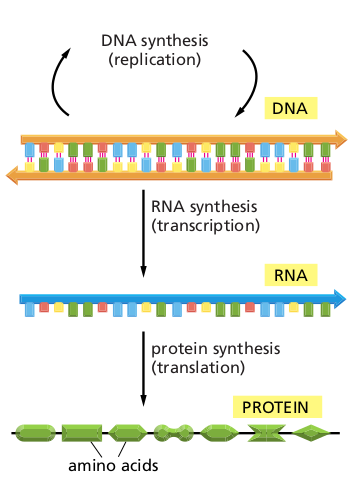
\includegraphics[width=0.5\textwidth]{TranslationAndTranscription} 
    \end{center}
    \caption{ فرآیند رونویسی، ترجمه و مضاعف کردن}
    \label{figure:translationAndTranscription}
\end{wrapfigure}

همه سلول‌ها حاوی ماده‌ ژنتیکیِ
\lr{DNA}
هستند به طوریکه از روی بخش‌هایی از این ماده ژنتیکی در فرآیند رونویسی
\footnote{\lr{transcription}}
مولکول
\lr{RNA}
ساخته می‌شود. در واقع کد ذخیره شده بر روی مولکول
\lr{DNA}
به روی یک مولکول
\lr{RNA}
کپی می‌شود. در ادامه نوع خاصی از این مولکول
\lr{RNA}
به مولکول پروتئین ترجمه می‌شود. نام این فرایند، ترجمه
\footnote{\lr{translation}}
است.

 در فرآیند ساخت پروتئین از روی کد ژنتیکی، مولکول
\lr{RNA}
به عنوان واسطه عمل می‌کند علت این امر آن است که ماده ژنتیکی حساس است و نباید در دسترس همه اندامک‌ها قرار گیرد. به علاوه برای ساخت پروتئین مولکول
\lr{RNA}
وارد ریبوزوم می‌شود که این کار برای مولکول طویل
\lr{DNA}
مقدور نیست چرا مشخص نیست که کدام قسمت آن باید ترجمه شود.

در جانداران چندسلولی ماده‌ ژنتیکی تمام سلول‌ها یکسان است. در واقع در سلول‌ها ماده‌ ژنتیکی یکسان است و فقط میزان رونویسی از روی ژن‌های متفاوت فرق دارد و همین بیان متفاوت ژن‌ها شخصیت سلول را شکل میدهد. در فرآیند فوق مانند کتاب آشپزی، که خود به تنهایی کار خاصی را انجام نمی‌دهد و باید از روی آن غذا پخته شود، ماده‌ ژنتیکی نیز خود کاری در سلول انجام نمی‌دهد  بلکه باید از روی آن پرو‌تئین ساخته شود. 

\noindent
مولکول‌های پرو‌تئین دارای شکل سه بعدی هستند که رفتار سلول را کنترل می‌کنند. پروتئین‌ها کارهای مختلفی را انجام می‌دهند.

\noindent
علاوه بر ماده ژنتیکی، همه سلول‌ها دارای  غشا و سیتوپلاسم هستند.

\subsubsection{تمام سلول‌ها از یک جد مشترک نشات گرفته‌اند}

همان طور که در تصویر
\ref{figure:translationAndTranscription}
مشاهده می‌شود مولکول
\lr{DNA}
می‌تواند خود را مضاعف کند. سلول برای این که تکثیر پیدا کند ابتدا ماده ژنتیکی خود را مضاعف می‌کند و سپس به دو سلول دختری تقسیم می‌شود.

\noindent
در زمان مضاعف شدن ممکن است جهش‌هایی در ماده ژنتیکی ِتکثیر پیدا کرده ایجاد شود و به سلول دختری منتقل شود. این جهش‌ها به سه نوع تقسیم می‌شوند:

\begin{itemize}
\item خوب:
تغییر در جهتی است که سازگاری جاندار را با محیط افزایش می‌دهد و قدرت زیست  یا توانایی تولید مثل آن را بیشتر می‌کند.
\item بد:
تغییر باعث کاهش قدرت زیست یا تولید مثل جاندار می‌شود.
\item خنثی:
تغییری در قدرت زیست و تولید مثل ایجاد نمی‌شود.
\end{itemize}

تکامل فرآیندی است که طی آن گونه‌های با سازگاری کمتر تغییر کرده و گونه‌های با سازگاری بیشتر را به وجود می‌آوردند و این گونه‌ها به دلیل داشتن ویژگی‌های زیستی سازگارتر جایگزین گونه قبلی می‌شوند .
اساس تغییر در گونه‌ها از یک نسل به نسل بعد تغییر ماده ژنتیکی آن‌ها است  که به آن جهش گفته می‌شود. این جهش‌ها در تولید‌مثل‌های جنسی پیچیدگی بیشتری دارند.

\bigskip
به طور کلی سلول‌ها به دو دسته کلی تقسیم می‌شوند:
\begin{itemize}
\item پروکاریوت‌ها 
\footnote{\lr{Prokaryote}}
\item یوکاریوت‌ها
\footnote{\lr{Eukaryote}}
\end{itemize}

\subsubsection{سلول پروکاریوتی\protect\footnote{\lr{Eukaryotic cell}}}

\begin{wrapfigure}[17]{l}{0.6\textwidth}
	\centering
	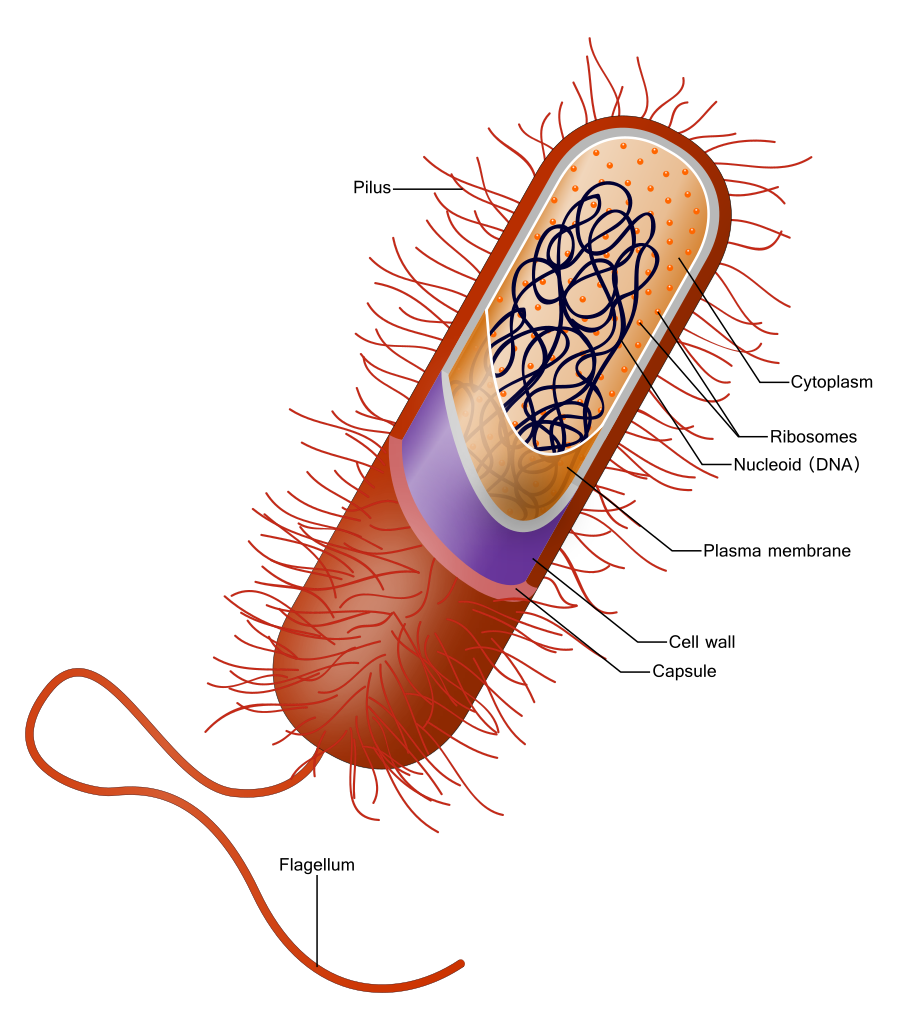
\includegraphics[width = 0.6\textwidth]{Prokaryote_cell}
\end{wrapfigure}

پروکاریوت به معنی پیش از هسته است و به این موضوع اشاره دارد که پروکاریوت‌ها فاقد هسته هستند و ماده ژنتیکی آن‌ها درون سیتوپلاسم حضور دارد. افراد این گونه عموما تک‌سلولی هستند اما در مواردی به صورت زنجیره به هم پیوسته در کنار یکدیگر زندگی می‌کنند. 

پروکاریوت‌ها شکل و ساختار ساده‌ای دارند با این حال از نظر شیمیایی متنوع‌ترین و خلاق‌ترین گونه جانداران هستند به طوریکه در طیف وسیعی از زیستگاه‌ها قدرت زندگی دارند.

\noindent
سلول پروکاریوتی در مدت زمان کمتر از 20 دقیقه می‌تواند تکثیر شود، در نتیجه درحدود 11 ساعت می‌تواند بیشتر از هشت میلیارد از خود تکثیر کند یعنی عددی بیشتر از تعداد انسان‌ها روی کره زمین!

\noindent
طبق سیستم ‌سه ‌دسته‌ای
\footnote{\lr{Three-domain system}}
پروکاریوت‌ها به دو دسته زیر تقسیم می‌شوند:

\begin{itemize}
\item باکتری (یوباکتری)
\footnote{\lr{Bacteria}}
\item آرکئا (آرکی باکتری) 
\footnote{\lr{Archaea}}
	\begin{itemize}
	\item
	می‌توانند در جاهایی زندگی کنند که اکثر سلول ها قدرت زندگی ندارد مثلا چشمه های اتشفشانی یا قطب جنوب.
	\item
	به نظر می رسد که این گونه میل به زندگی در مناطقی را دارد که مشابه با شرایط اولیه کره زمین است. 	
	\end{itemize}
\end{itemize}

\subsubsection{سلول یوکاریوتی\protect\footnote{\lr{Eukaryotic cell}}}

یوکاریوت به معنی خوش‌هسته است و به این اشاره دارد که این نوع از سلول‌ها دارای هسته هستند. علاوه بر این سلول‌های یوکاریوتی دارای اندامک
\footnote{\lr{Organelle}}
هستند
سلول‌های یوکایوتی عموما بزرگتر از سلول‌های پروکاریوتی هستند.
همانطور که در شکل
\ref{figure:KindsOfCell}
مشاهده می‌شود جاندارانِ یوکاریوتی به دو دسته چند‌سلولی و تک‌سلولی تقسیم می‌شوند.
\pagebreak

\begin{figure}[h]
\begin{center}
\begin{tikzpicture}
\path[mindmap,concept color=black!65!white,text=white]
node[concept] {\rl{{\Large \em انواع گونه‌ها}}}
[clockwise from=-60]
child[concept color=black!70!white] {
	node[concept] {\rl{پروکاریوتی}}
	[clockwise from=60]
	child[concept color=black!75!white]
	{ node[concept] {\rl{باکتری}} }
	child[concept color=black!75!white] 
	{ node[concept] {\rl{آرکئا} }}
}
child[concept color=black!70!white] {
	node[concept] {\rl{یوکاریوتی}}
	[clockwise from=-180]
	child [concept color=black!75!white]{ 
	node[concept] {\rl{تک‌سلولی} }
		child[concept color=black!80!white]
		{ node[concept] {\rl{آمیب‌ها} }}
		child[concept color=black!80!white] 
		{ node[concept] {\rl{مخمر‌ها} }}
	}
	child [concept color=black!75!white]{ 
	node[concept] {\rl{چندسلولی} }
		child[concept color=black!80!white]
		{ node[concept] {\rl{گیاهان} }}
		child[concept color=black!80!white]
		{ node[concept] {\rl{جانوران} }}
		child[concept color=black!80!white]
		{ node[concept] {\rl{قارچ‌ها} }}
	}
}
;
\end{tikzpicture}
\end{center}
\caption{تقسیم‌بندی انواع جانداران}
\label{figure:KindsOfCell}
\end{figure}

~\pagebreak
\subsubsection{تفاوت بین سلول یوکاریوتی و پروکاریوتی}

در جدول
\ref{table:difBetweenProAndEu}
برخی از تفاوت‌ها بین سلول‌های یوکاریوتی و پروکاریوتی ذکر شده است:

\begin{table}[h]
	\centering
	\begin{tabular}{|c|c|}
	\hline
سلول پروکاریوتی	& سلول یوکاریوتی
	\\
	\hline
اندازه سلول کوچک است
($ > 5 \mu m $)
&
اندازه سلول بزرگ است
($ <10 \mu m $)
	\\
	\hline
به صورت تک سلولی
	&
به صورت چند سلولی
	\\
	\hline
بدون هسته هستند و اندامک غشاءداری مانند میتوکندری ندارند
&
هسته و اندامک‌های غشاء دار دارند
	\\
	\hline
\lr{DNA}
به صورت حلقوی است و پروتئینی به همراه ندارد
&
 \lr{DNA}
 به صورت خطی است و به همراه پروتئین‌هایی ساختار کروماتین را میسازد
	\\
	\hline
ریبوزوم‌ها کوچک هستند
($ 70S $)
&
ریبوزوم‌ها بزرگ هستند
($ 80S $)
	\\
	\hline
اسکلت سلولی ندارند ؟
& 
اسکلت سلولی دارند
	\\
	\hline
تحرک توسط تاژک
\footnote{\lr{flagellum}}
 چرخان سفت و سخت (ساخته شده از فلاژلین
\footnote{\lr{Flagellin)}} 
 )
 &
 تحرک توسط تاژک یا مژک
 \footnote{\lr{Cilia}}
 انعطاف‌پذیر و موج‌زن ( ساخته شده توسط توبولین
 \footnote{\lr{Tubulin}}
 )
	\\
	\hline
تقسیم سلولی با شکافت دوتایی
\footnote{\lr{Binary fission}}
&
تقسیم سلولی با میوز
\footnote{\lr{Meiosis}}
یا میتوز
\footnote{\lr{Mitosis}}
	\\
	\hline
مضاعف‌شدن
\footnote{Reproduction}
همیشه به صورت غیر جنسی است
&
مضاعف شدن به صورت جنسی یا غیرجنسی است
	\\
	\hline
تنوع بسیار زیاد در مسیر‌های متابولیکی
\footnote{\lr{Metabolic pathway}}
&
مسیر‌های متابولیک مشترک
	\\
	\hline												
	\end{tabular}
	\caption{ تفاوت انواع سلول}
	\label{table:difBetweenProAndEu}
\end{table}


\subsubsection{سیستم غشائی درونی}

\begin{wrapfigure}[12]{l}{0.6\textwidth}
	\centering
	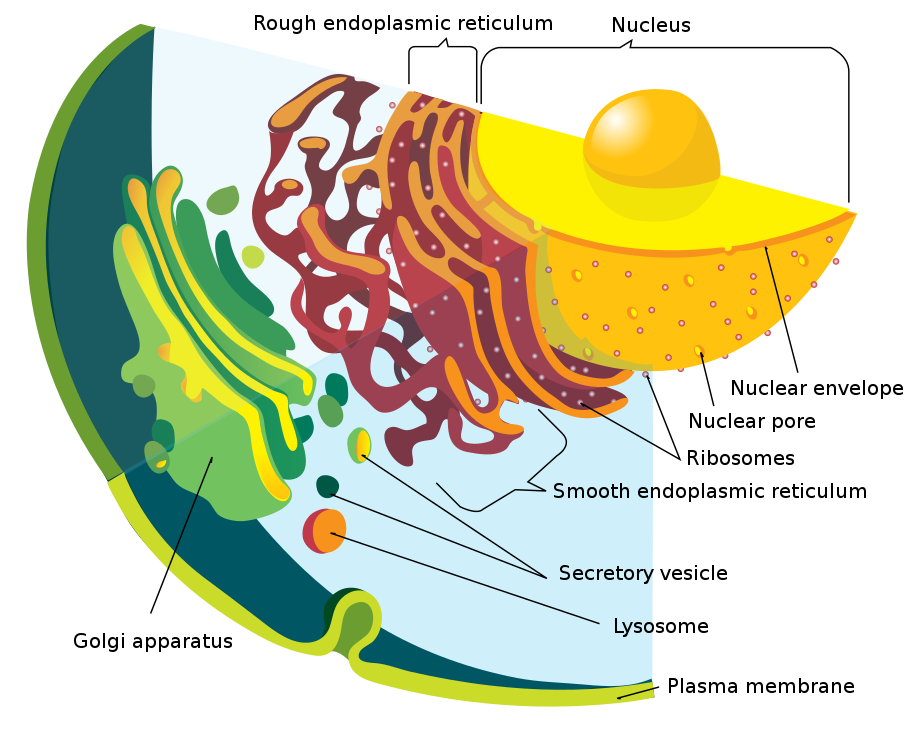
\includegraphics[width=0.6\textwidth]{Eukaryotic_cell}
	\caption{سیستم غشائی درونی}
	\label{figure:endomembraneSystem}
\end{wrapfigure}

سلول‌های یوکاریوتی شامل تعدادی ساختار غشاء‌دار
\footnote{\lr{Membrane-bound structure}}
هستند که به مجموع این ساختار‌ها، دستگاه غشائی درونی
\footnote{\lr{Endomembrane system}}
گفته می‌شود. در شکل
\ref{figure:endomembraneSystem}
اجزاء این دستگاه را مشاهده می‌کنیم. محفظه‌های
\footnote{\lr{Compartment}}
ساده مانند وزیکول
\footnote{\lr{Vesicle}}
و واکوئل
\footnote{\lr{Vacuole}}
می‌توانند با جوانه زدن بقیه غشاء‌ها به وجود بیایند.

عمدتا تغذیه سلول به وسیله فرآیند اندوسیتوز
\footnote{\lr{Endocytosis}}
انجام می‌شود. همان طور که در شکل
\ref{figure:Endocytosis}
مشاهده می‌کنید غذا توسط غشاء سلول بسته بندی و وارد سلول می‌شود.
این بسته‌بندی به صورت وزیکول و یا واکوئل است.
همچنین سلول‌ها می‌توانند موادی را که تولید می‌کنند با فرآیند اگزوسیتوز
\footnote{\lr{Exocytosis}}
به خارج از سلول ارسال کنند.

\pagebreak
\begin{figure}[t]
	\centering

	\subfloat[وزیکول]{{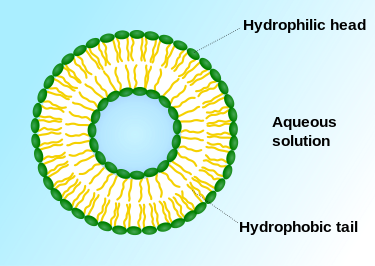
\includegraphics[width=5cm]{Vesicle} }}
    \qquad
    \subfloat[واکوئل]{{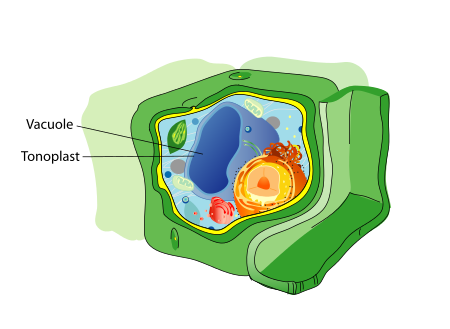
\includegraphics[width=5cm]{Vacuole} }}
    	\bigskip
	
	\begin{subfigure}[b]{0.85\textwidth}
		\centering
		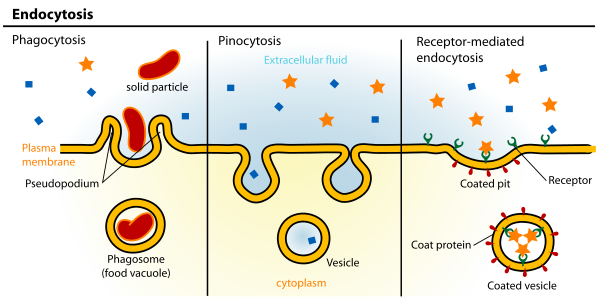
\includegraphics[width=0.8\textwidth]{Endocytosis}
		\caption{انواع اندوسیتوز}
		\label{figure:Endocytosis}
	\end{subfigure}	
	\caption{سیستم غشائی درونی}
\end{figure} 

~

\pagebreak
\subsubsection{اندامک‌ها\protect\footnote{\lr{Organelle}}}

\begin{figure}[t]
	\centering
	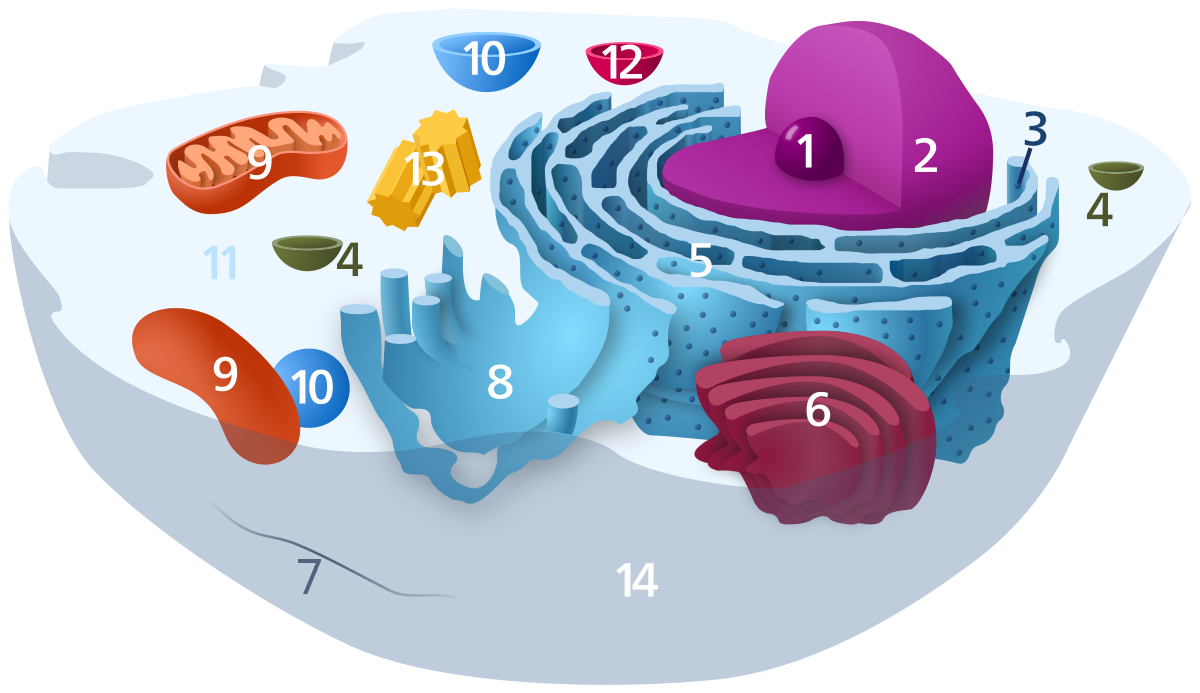
\includegraphics[width=0.5\textwidth]{Animal_cell}
	\caption{ اندامک‌های یک سلول جانوری.
	\lr{1.Nucleolus}
	\lr{2.Nucleus}
	\lr{3.Ribosome}
	\lr{4.Vesicle}
	\lr{5.Rough endoplasmic reticulum}
	\lr{6.Golgi apparatus}
	\lr{7.Cytoskeleton}
	\lr{8.Smooth endoplasmic reticulum}
	\lr{9.Mitochondrion}
	\lr{10.Vacuole}
	\lr{11.Cytosol }
	\lr{12.Lysosome}
	\lr{13.Centrosome}
	\lr{14.Cell membrane}	
	}
	\label{figure:Organelle}
\end{figure}

اندامک‌ها اجزائی هستند که وظایفی را به عهده دارند.  در زیر بعضی از آنها به اختصار توضیح داده شده‌اند:

\begin{description}
\item[\lr{Golgi apparatus}]
گلژی وظیفه ارسال پروتئین‌های جدید به جایگاه‌های مناسب را بر عهده دارد.
شکل
\ref{figure:Organelle}
(۶)
\item[\lr{Lysosome}]
لیزوزوم مواد غیرلازم را تجزیه می‌کند.
شکل
\ref{figure:Organelle}
(12)
\item[\lr{Cytosol }]
مایعی که سایر اندامک‌ها در آن جای دارند.
\ref{figure:Organelle}
شکل
(11)
\item[\lr{Cytoskeleton}]
اسکلت سلولی مانند اسکلت بدن برای سلول است و اندامک‌ها را در جایگاه مناسب نگاه می‌دارد. اسکلت سلولی تنها از یک بخش تشکیل نشده و اجزاء مختلفی در کنار هم قرار گرفته‌اند تا آن را تشکیل دهند.
شکل
\ref{figure:Organelle}
(7)

اسکلت سلولی یوکاریوت‌ها از سه نوع فیلامین
\footnote{\lr{Filament}}
اصلی تشکیل شده‌اند:

\begin{itemize}
\item
میکروفلامین یا ریزرشته‌ها
\footnote{\lr{microfilament}}
 پلیمر‌هایی از پروتئین اکتین
\footnote{\lr{Actin}}
هستند که باریک می‌باشند و هفت نانومتر قطر دارند.
\item
میکروتوبول یا ریزلوله‌ها
\footnote{\lr{microtubule}}
 از پروتئین توبولین
\footnote{\lr{tubulin}}
ساخته شده‌اند و 25 نانومتر قطر دارند.
\item
رشته‌های متوسط
\footnote{\lr{intermediate filament}}
 از پروتئین‌های مختلفی ساخته شده‌اند و این برحسب سلول مورد نظر متفاوت است.
\end{itemize}

\begin{figure}[h]
	\centering
	\subfloat[ساختار میکروفلامین]{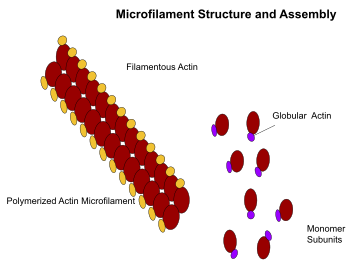
\includegraphics[width = 5cm]{Microfilament}}
	\qquad
	\subfloat[ساختار میکروتوبول]{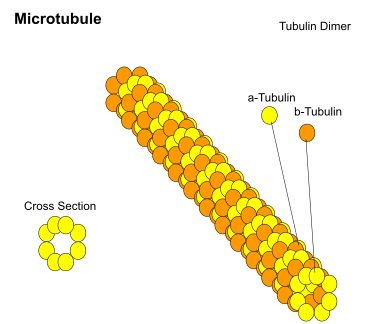
\includegraphics[width = 5cm]{Microtubule}}
\end{figure}

\begin{table}[h]
	\centering
	\begin{tabular}{|r|r|r|}
\hline
نوع اسکلت سلولی & قطر به نانومتر & ماده‌سازنده \\
\hline
میکروفیلامین & 6 & اکتین\\
فلامین متوسط & 10 & با توجه به  نوع سلول متفاوت \\
	میکروتوبول‌ & 23 & توبولین آلفا و بتا\\
\hline
	\end{tabular}
	\caption{انواع فیلامین‌های اسکلت سلولی}
\end{table}

\item[\lr{Nucleus}]

هسته در سلول‌های یوکاریوتی یافت می‌شود . اغلب، سلول‌ها یک هسته دارند اما سلول‌های وجود دارند که هسته ندارند و یا بیش از یک هسته دارند.
شکل
\ref{figure:Organelle}
(2)

 هسته را پوشش هسته
\footnote{\lr{Nuclear envelop}}
فرا گرفته‌است که این پوشش از دو لایه تشکیل شده است.

\begin{figure}[h]
	\centering
	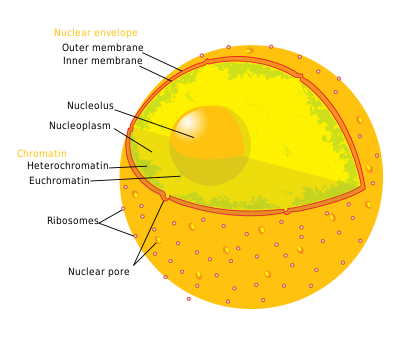
\includegraphics[width=0.4\textwidth]{Nucleus}
\end{figure}

ماده ژنتیکی
(\lr{DNA})
درون هسته قرار دارد.  در شرایط خاص به این ماده ژنتیکی کروموزوم
\footnote{\lr{Chromosome}}
،کروماتین
\footnote{\lr{Chromatin}}
و یا کروماتید
\footnote{\lr{Chromatid}}
گفته می‌شود.
وقتی که سلول در حال تقسیم نیست،	
\lr{nuclear DNA}
به همراه انواعی از پروتئین‌ها به صورت کروماتین شکل میگیرند. سپس هنگامی که سلول می‌خواهد تقسیم انجام دهد، کروماتین به صورت ساختار فشرده‌ی کروموزوم در  می‌آید.

\begin{figure}[htbp]
	\centering
	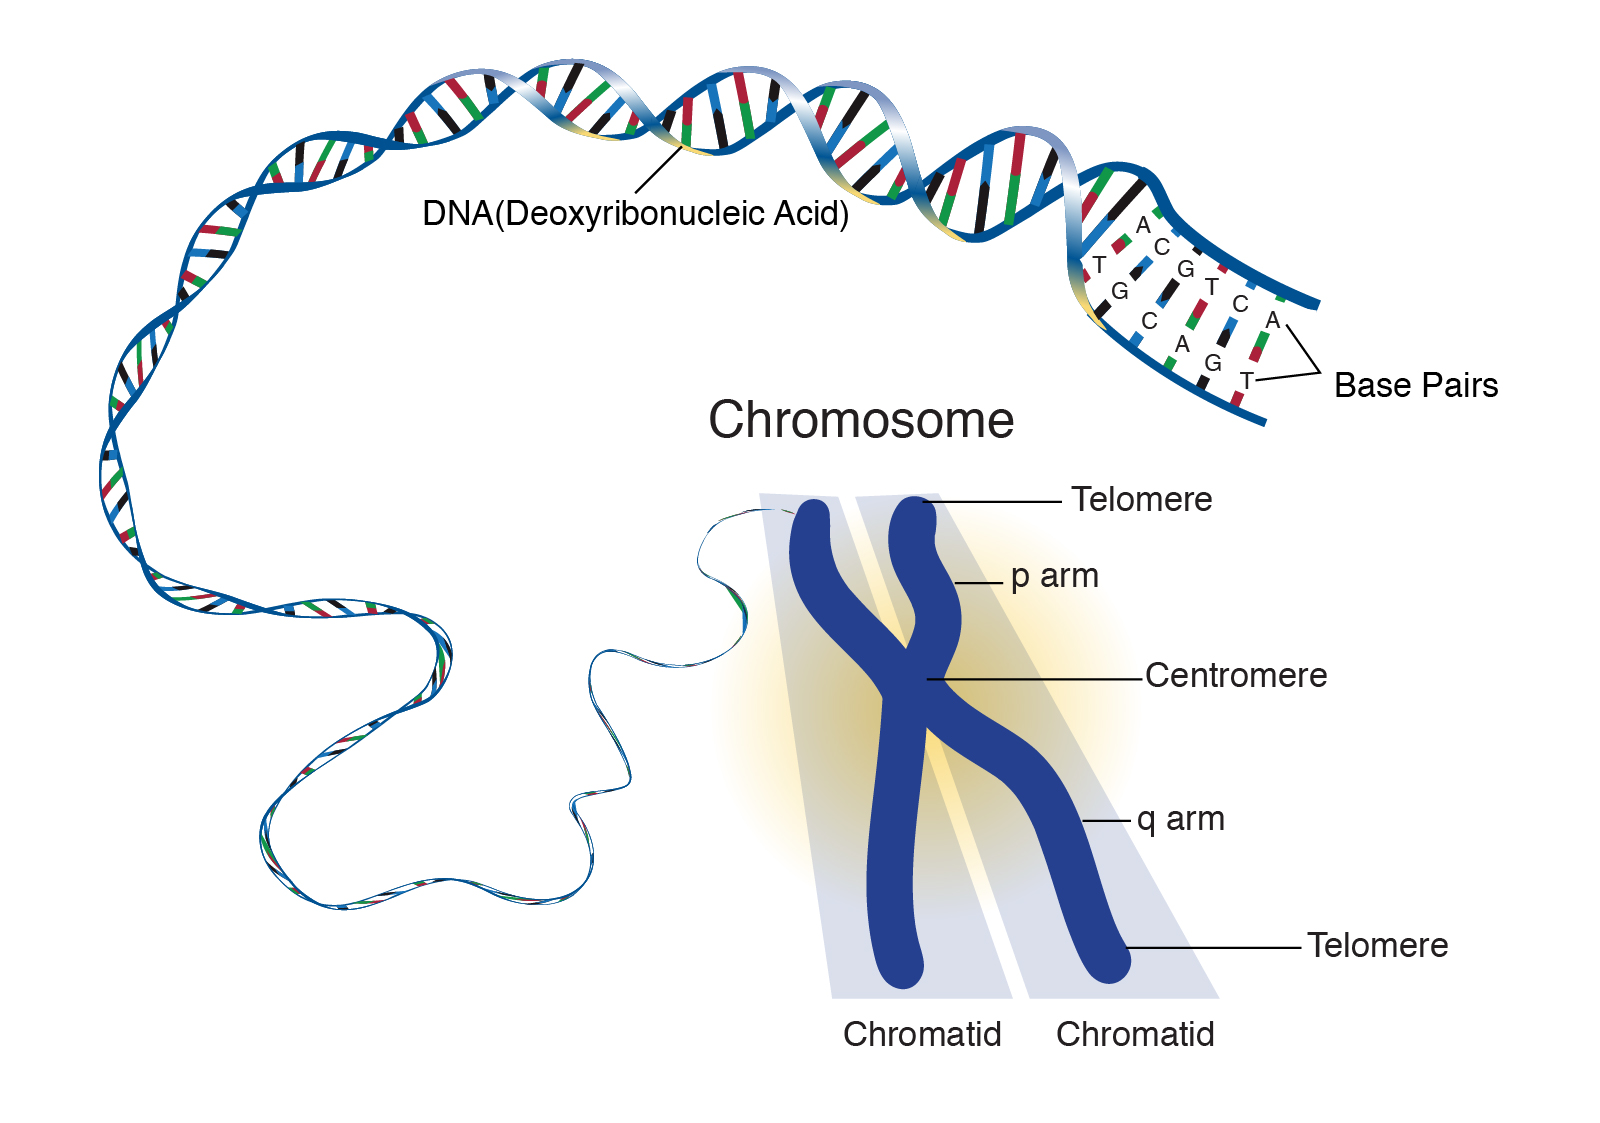
\includegraphics[width=0.7\textwidth]{Chromosome}
	\caption{ساختار کروموزوم}
	\label{figure:Chromosome}
\end{figure}

همانطور که در شکل
\ref{figure:Chromosome}
مشاهده می‌کنید کروموزوم از دو قسمت
\lr{P-arm}
و
\lr{Q-arm}
ساخته شدند که اولی بازوی کوتاه و دومی بازوی بلند کروموزوم را تشکیل می‌دهند.

\item[\lr{Mitochondria}]
این اندامک خود دارای
\lr{DNA}
است و دو لایه غشاء دارد. میتوکندری وظیفه تولید انرژی شیمیایی برای سلول را برعهده دارد. طی این فرآیند میتوکندری قند یا چربی را اکسید می‌کند و
\lr{ATP}
را به عنوان انرژی شیمیایی آزاد می‌کند.
شکل
\ref{figure:Organelle}
(9)

\item[\lr{Chloroplast}]
کلروپلاست در گیاهان وجود دارد. و سلول‌های گیاهی انرژی خود را از طریق این اندامک تامین می‌کنند. کلروپلاست دارای کلروفیل
\footnote{\lr{Chlorophyll}}
می‌باشد. کلروفیل نور خورشید را به دام می‌اندازد و آن را در ملکول‌های
\lr{ATP}
و
\lr{NADPH}
ذخیره می‌کند. در کنار این فرآیند اکسیژن آزاد می‌شود و در نتیجه میتوکندری می‌تواند از آن استفاده کند.

\item[\lr{Endoplasmic reticulum}]
شبکه آندومپلاسمی از دو قسمت نرم
\footnote{\lr{Smooth endoplasmic reticulum}}
و سخت
\footnote{\lr{Rough endoplasmic reticulum}}
تشکیل شده است. شکل
\ref{figure:Organelle}
(5 و 8).
بر روی شبکه آندوپلاسمی زبر تعدادی ریبوزوم  وجود دارد که این ریبوزوم‌ها از روی 
\lr{RNA}
ها پروتئین می‌سازند. هنگامی که این پروتئین‌ها ساخته می‌شوند به وسیله شبکه آندوپلاسمی زبر به سمت گلژی فرستاده می‌شوند.
 شبکه آندوپلاسمی نرم نیز محصولاتی مانند لیپید و یا فسفولیپید تولید می‌کند.
 
\begin{figure}[htbp]
	\centering
	\subfloat[ساختار میتوکندری]{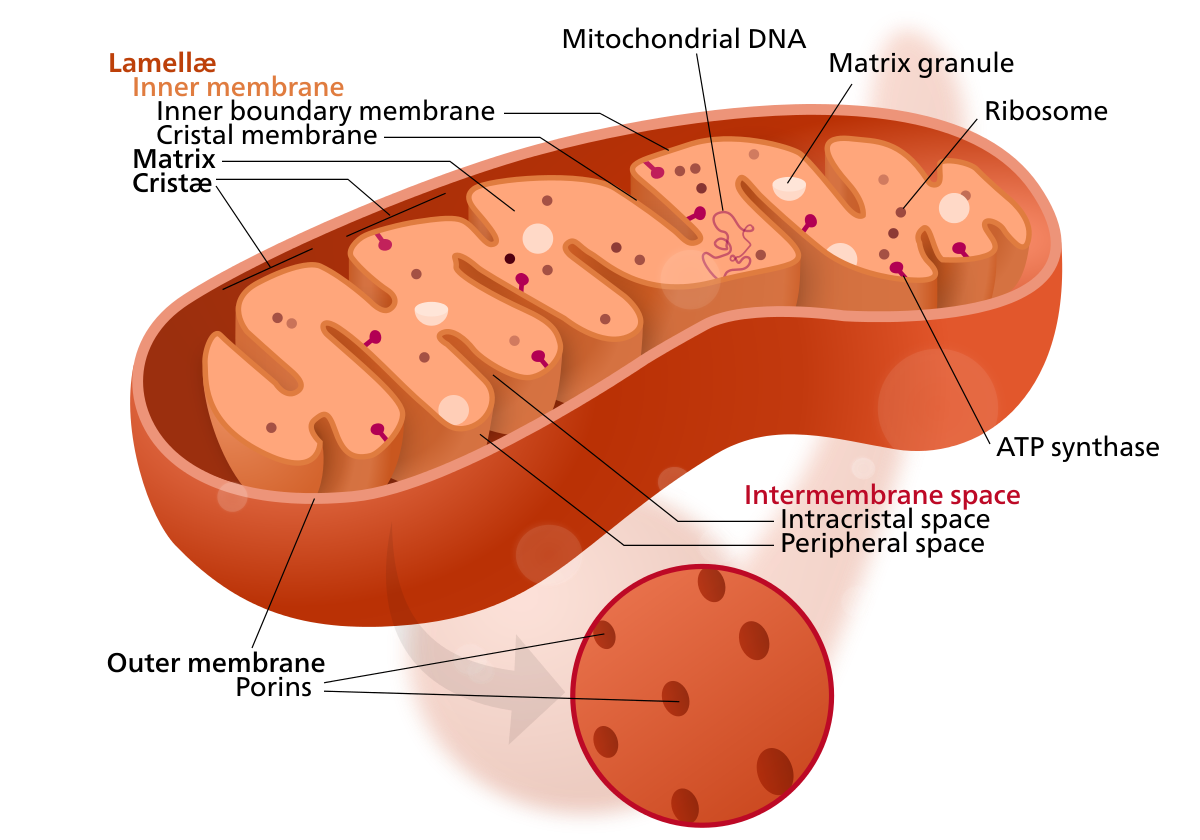
\includegraphics[width=7cm]{Mitochondrion_structure}}
	\qquad
	\subfloat[ساختار کلروپلاست]{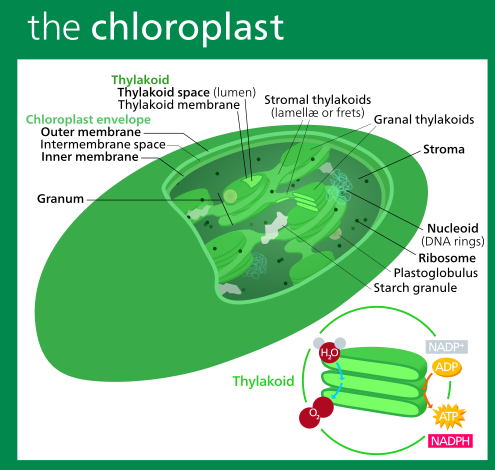
\includegraphics[width=7cm]{Chloroplast}}
\end{figure} 
 
\begin{figure}[t]
	\floatbox[{\capbeside\thisfloatsetup{capbesideposition={right,top},capbesidewidth=6cm}}]{figure}[\FBwidth]
{\caption
{
\lr{1.Nucleus}
\lr{2.Nuclear~pore}
\lr{3.Rough~endoplasmic~reticulum~(RTE)}
\lr{4.Smooth~endoplasmic~reticulum~(SER)}
\lr{5.Ribosome~on~rough~ER}
\lr{6.Proteins~that~are~transported}
\lr{7.Trasport~vesicle}
\lr{8.Golgi~apparatus}
\lr{9.Cis~face~of~Golgi~apparatus}
\lr{10.Trans~face~of~Golgi~apparatus}
\lr{11.Cisternae~of~the~Golgi~apparatus}
}
\label{fig:EndoplasmicReticulum}}
{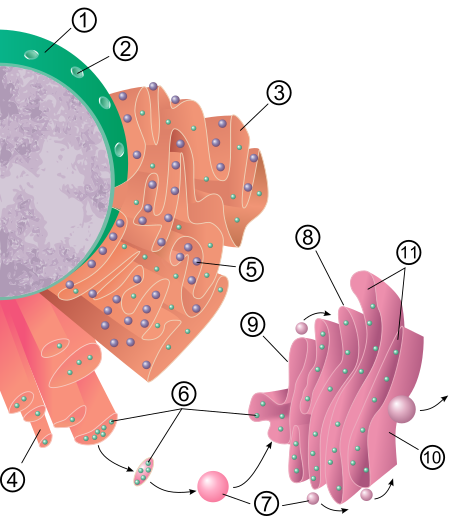
\includegraphics[width=0.4\textwidth]{Endoplasmic_reticulum_golgi}}

\end{figure}  
 
\end{description}

\pagebreak
\subsubsection{کلروپلاست و میتوکندری شباهت زیادی به باکتری دارند}

همانطور که مشاهده شد این دو اندامک شباهت زیادی به باکتری‌ها دارند و نظریه‌ای و جود دارد که طی آن سلول یوکاریوتی این دو اندامک را به صورت غذا وارد خود ساخته و سپس با آن همزیست شده است. به شکل
\ref{figure:PrimaryEndosymbiosis}
رجوع کنید.

\begin{figure}[hbt]
	\centering
	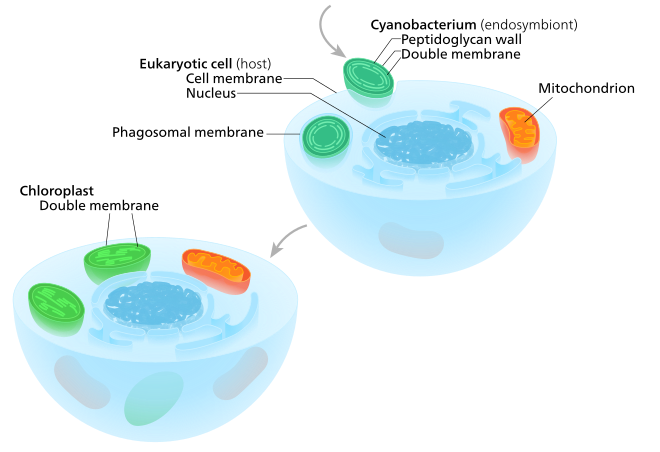
\includegraphics[width = 0.6\textwidth]{Chloroplast_endosymbiosis}
	\caption{\lr{A eukaryote with mitochondria engulfed a cyanobacterium in an event of serial primary endosymbiosis, creating a lineage of cells with both organelles.}}
	\label{figure:PrimaryEndosymbiosis}
\end{figure}

\subsubsection{موجودات مدل}
در زیست شناسی نمونه‌های خاصی وجود دارد که سایر گونه‌ها شباهت زیادی به آن‌ها دارند در نتیجه زیست شناسان ابتدا روی این گونه‌ها آزمایش می‌کنند. در زیر به مواردی اشاره شده است:

\begin{itemize}
\item ای کولی
\item ساکارومایسس
\item آرابیدوبسیس
\item مگس
\item کرم
\item ماهی
\item موش
\item انسان
\end{itemize}

\subsubsection{سنترال دوگما\protect\footnote{\lr{Central dogma}}}

\begin{wrapfigure}[13]{l}{0.7\textwidth}
	\centering
	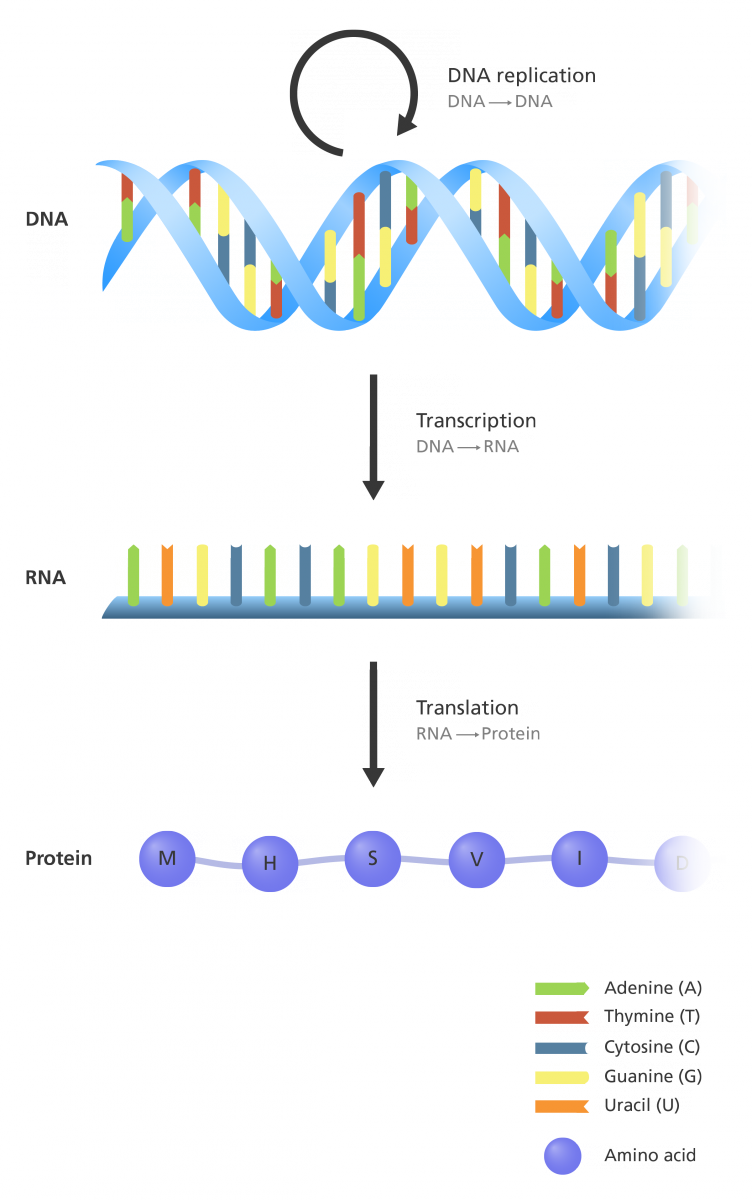
\includegraphics[width=0.7\textwidth]{Central_dogma}
	\caption{فرايند مضاعف کردن، رونویسی و ترجمه}
	\label{figure:CentralDogma}
\end{wrapfigure}

هر سلولی چه از نوع یوکاریوتی باشد و چه از نوع پروکاریوتی دارای فرآیند سنترال دوگما است که طی آن اطلاعات ژنتیکی به پروتئین تبدیل می‌شود.
طی این فرآیند ابتدا از روی ماده‌ژنتیکی مولکول
\lr{RNA}
ساخته می‌شود سپس این مولکول‌ها به ریبوزوم رفته و از روی آن‌ها پروتئین ساخته می‌شود.
همان طور که در شکل
\ref{figure:CentralDogma}
مشاهده می‌شود این فرآیند شامل سه مرحله است.
برای اینکه بتوان این فرآیند را درک کرد ابتدا نیاز داریم که به بررسی ساختار مولکول
\lr{DNA}
بپردازیم.
\pagebreak

\subsubsection{نوکلئیک اسید‌ها}

\begin{wrapfigure}{l}{8cm}
	\centering
	
	\begin{subfigure}[b]{8cm}
		\centering
		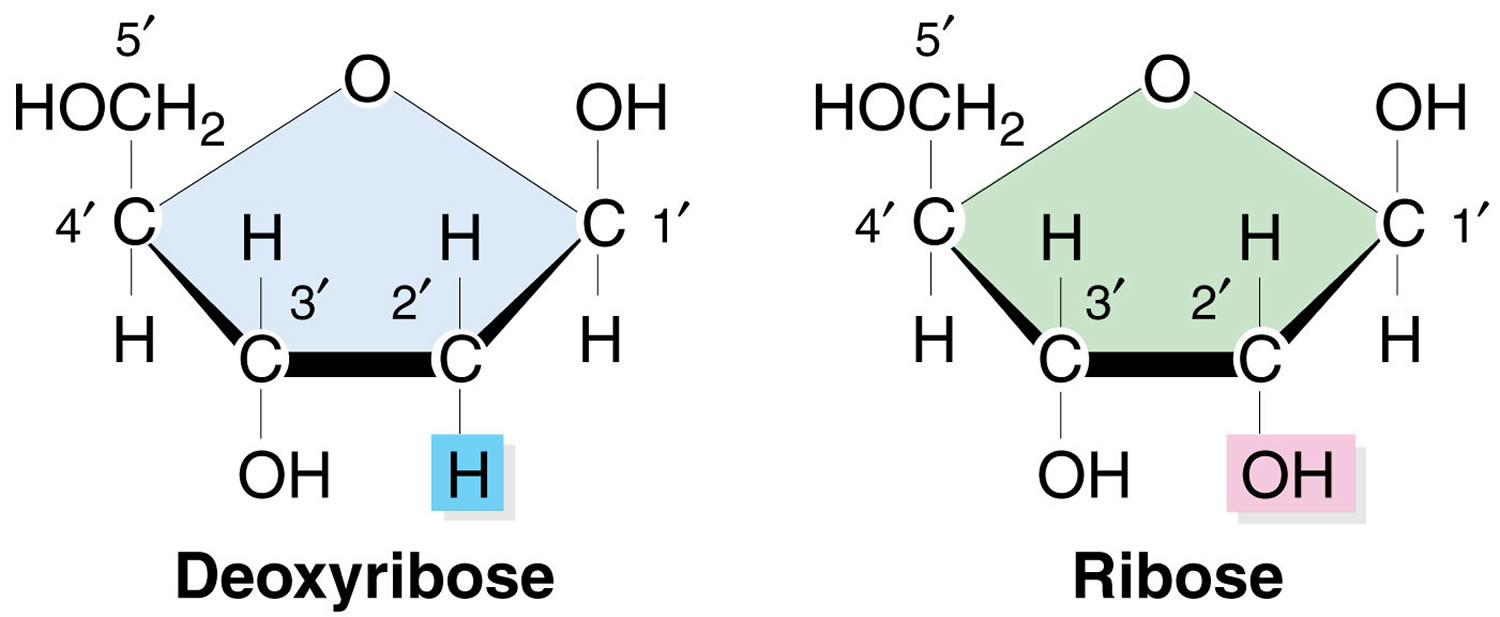
\includegraphics[width = 7cm]{Ribose_and_deoxyribose}
		\caption{قند ریبوز و دئوکسی‌ریبوز}	
	\end{subfigure}
	\begin{subfigure}[b]{8cm}
		\centering
		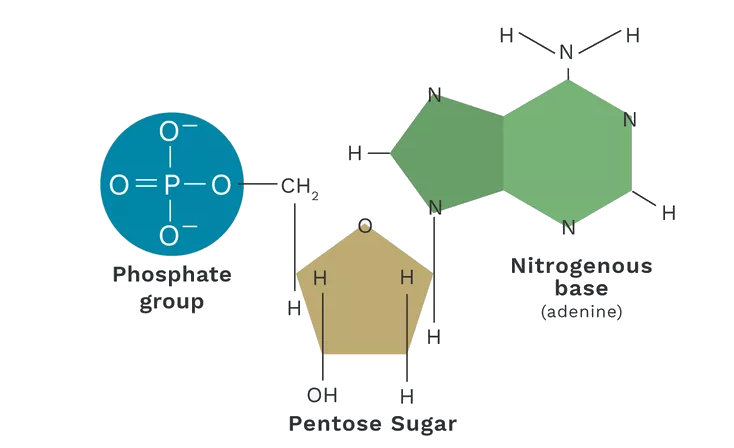
\includegraphics[width=8cm]{Nucleotide}
		\caption{اجزاء ریزملکول نوکلئوتید}
		\label{figure:Nucleotide}
	\end{subfigure}
	
\end{wrapfigure}

در سال 1870 فردریک میشر از هسته سلول، ماده ای استخراج کرد که خاصیت اسیدی داشت به همین علت نام آن را نوکلئیک اسید
\footnote{\lr{Nucleic acid}}
به معنی اسید هسته‌ای گذاشت. بعد‌ها مشخص شد که نوکلئیک اسید‌ها دو نوع هستند:
\begin{itemize}
\item ریبو نوکلئیک اسید یا 
\lr{RNA}
که در ساختار آن قند ریبوز
\footnote{\lr{Ribose}}
 به کار رفته است.
\item دئوکسی ریبو نوکلئیک اسید یا
\lr{DNA}
که در ساختار آن قند دئوکسی ریبوز
\footnote{\lr{Deoxyribose}}
 به کار رفته است.
\end{itemize}

نوکلئیک اسید‌ها همانند پروتئین‌ها و کربوهیدرات‌ها پلی‌مر هستند. واحد‌ مونومری نوکلئیک اسید‌ها، نوکلئوتید
\footnote{\lr{Nucleotide}}
است.
همانطور که در شکل
\ref{figure:Nucleotide}
مشاهده می‌کنید، مولکول نوکلئوتید از سه بخش تشکیل شده است:
\begin{itemize}
\item  یک تا سه گروه فسفات
\item  قند پنتوز که ریبوز در
\lr{RNA}
و
دئوکسی ریبوز در
\lr{DNA}
است
\item  باز آلی نیتروژن‌دار
\end{itemize}

در تمام انواع این مولکول قسمت فسفات و قند یکسان است (با توجه به دی‌ان‌ای یا آرآن‌ای بودن) اما با توجه به نوع باز پنج نوع مولکول نوکلئوتید به وجود می‌آیند که در نوکلئیک‌اسید‌ها
به کار رفته است:
\begin{itemize}
\item پورین‌ها با دو حلقه
\footnote{\lr{Purine}}
	\begin{itemize}
	\item آدنین
	\footnote{\lr{Adenine (A)}}
	\item گوانین
	\footnote{\lr{Guanine (G)}}
	\end{itemize}
\item پریمیدین‌ها با یک حلقه
\footnote{\lr{Pyrimidine}}
	\begin{itemize}
	\item سیتوزین
	\footnote{\lr{Cytosine (C)}}
	\item تیمین
	\footnote{\lr{Thymine (T)}}
	در دئوکسی ریبونوکلئیک اسید	
	\item یوراسیل
	\footnote{\lr{Uracil (U)}}
در ریبونوکلئیک اسید
	\end{itemize}
\end{itemize}

\noindent
در شکل
\ref{figure:bases}
ساختار این باز‌ها مشخص شده است.

\begin{figure}[ht]
	\centering
	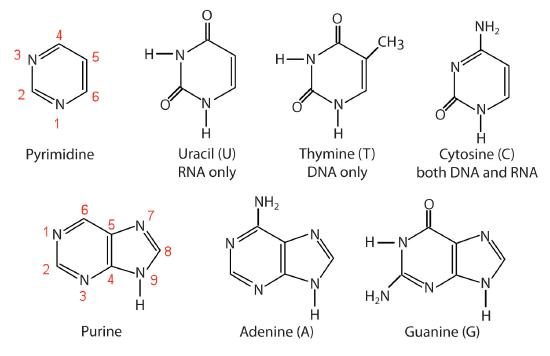
\includegraphics[width = 10cm]{Bases}
	\caption{انواع باز‌هایی که در مولکول
	\lr{DNA}
	و
	\lr{RNA}
	به کار رفته است.	
	}
	 \label{figure:bases}
\end{figure}

از کنار هم قرار گرفتن مولکول‌های نوکلئوتید پلی‌مری خطی به وجود می‌‌آيد. اتصال بین دو مولکول نوکلئوتید از طریق برقراری پیوند کووالانسی
\footnote{\lr{Covalent}}
بین گروه فسفات یک نوکلئوتید و قند نوکلئوتید بعدی است. نوکلئوتید‌ها به صورت آزاد سه گروه فسفات دارند اما هنگام برقراری اتصال با یکدیگر دو گروه فسفات خود را از دست می‌دهند و با یک گروه فسفات در رشته پلی‌نوکلئوتیدی قرار می‌گیرند. پیوند بین دو نوکلئوتید را پیوند فسفو دی استر
\footnote{\lr{Phosphodiester bound}}
می‌نامند.

همانطور که در شکل
\ref{figure:PhosphodiesterBond}
مشاهده می‌شود در یک انتهای رشته پلی‌نوکلئوتیدی گروه فسفات وجود دارد حال آنکه در انتهای دیگر وجود ندارد به همین علت رشته پلی‌نوکلئوتیدی دارای قطبیت است.

\pagebreak
\begin{wrapfigure}[22]{l}{9cm}
	\centering
	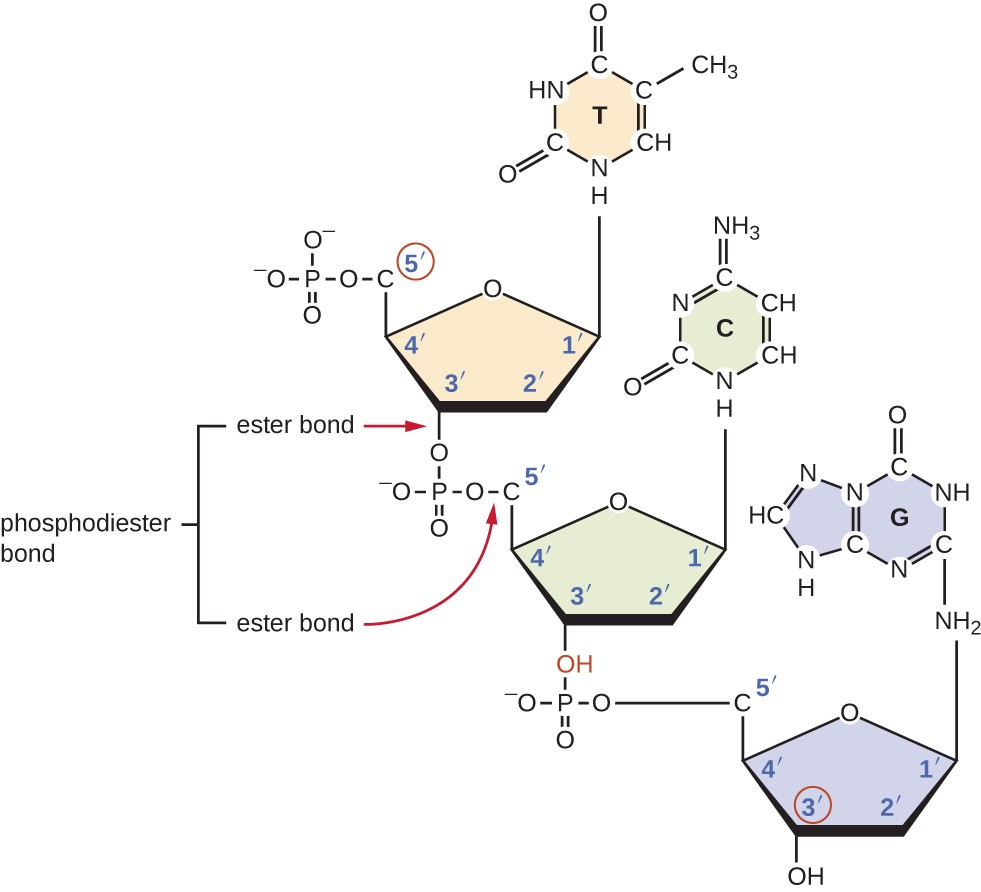
\includegraphics[width=9cm]{DNA_five_to_three}
	\caption{
	پیوند فسفودی‌استری
	\protect	
	\footnote{\lr{Phosphodiester}}
	بین  گروه فسفات متصل به کربن
	$ 5^\prime $
	یک نوکلئوتید و گروه هیدروکسیل
	\protect
	\footnote{\lr{Hydroxyl}}
	نوکلئوتید بعدی برقرار می‌شود.	
	}
	\label{figure:PhosphodiesterBond}
\end{wrapfigure}

همانطور که در شکل
\ref{figure:PhosphodiesterBond}
مشاهده می‌شود کربن
$ 5^\prime $
نوکلئوتید اول و کربن
$ 3^\prime $
نوکلئوتید آخر بیکار هستند به همین خاطر اصطلاحا می‌گویند
\lr{DNA}
از سمت
$ 5^\prime $
به سمت
$ 3^\prime $
شکل می‌گیرد.

دو رشته مولکول
\lr{DNA}
به صورت آنتی پارالل
\footnote{\lr{Antiparallel}}
در مقابل یکدیگر قرار میگیرند. در واقع یک رشته در جهت
$ 5^\prime $
به سمت
$ 3^\prime $
است و دیگری در جهت
$ 3^\prime $
به سمت
$ 5^\prime $
.

پیوند بین دو رشته از نوع هیدروژنی است. هر باز فقط با مکمل خود پیوند برقرار می‌کند به این صورت که آدنین مکمل تیمین است و سیتوزین مکمل گوآنین.
بین آدنین و تیمین دو پیوند هیدروژنی شکل می‌گیرد و بین سیتوزین و گوآنین سه پیوند. این نکته در کار‌های محاسباتی اهمیت دارد.
به یک جفت باز که با هم پیوند هیدروژنی تشکیل می‌دهند 'جفت باز` 
\footnote{\lr{Base pair}}
گفته می‌شود.

باز‌هایی که مکمل هم هستند هنگامی که کنار هم قرار میگیرند فاصله یکسانی را میسازند که این باعث استحام نردبان
\lr{DNA}
می‌شود حال آنکه اگر دو باز که مکمل هم نیستند در کنار یکدیگر قرار بگیرند فاصله‌ای که می‌سازند با سایر جفت بازها متفاوت است و استحام مولکول
\lr{DNA}
از بین می‌رود.

هنگامی که در مولکول
\lr{DNA}
جفت بازها کنار یکدیگر قرار می‌گیرند به هم فشار می‌آورند و الکترون تبادل می‌کنند که به آن
\lr{`Base stacking'}
گفته می‌شود.

\pagebreak
\subsubsection{مولکول دی ان ای}
مولکول
\lr{DNA}
به صورت دورشته‌ای
\footnote{\lr{Double stranded}}
است. به نظر می‌رسد که طبیعت برای این که از تغییر ماده‌ژنتیکی هنگام تولید مثل جلوگیری کند تصمیم گرفته است تا این مولکول به صورت دورشته‌ای باشد چرا که از روی یک رشته می‌توان رشته دیگر را ترمیم کرد.

\begin{figure}[h]
	\centering
	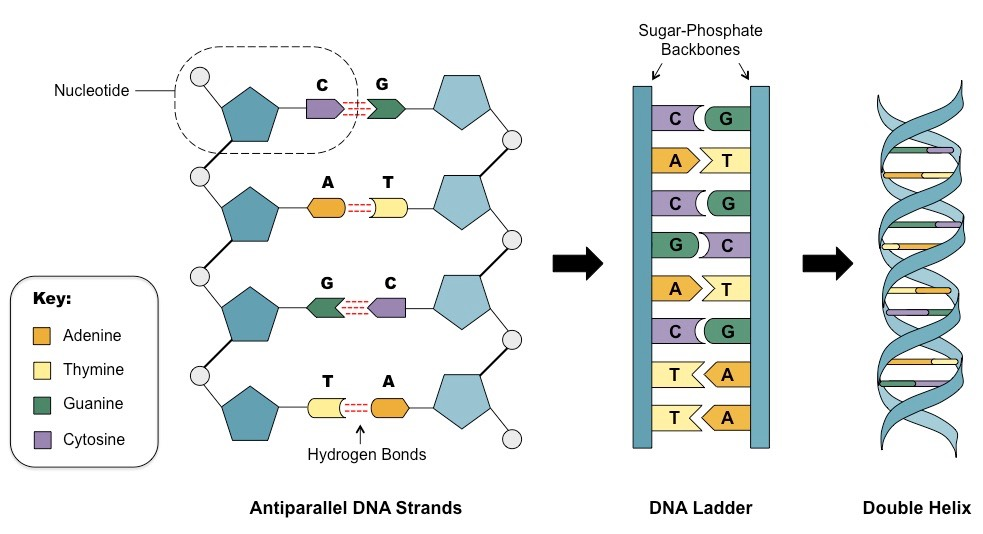
\includegraphics[width=11cm]{double-stranded-dna}
\end{figure}

ساختار مولکول
\lr{DNA}
به صورت پیچشی است و پیچ‌های مولکول، اهمیت زیادی دارد و با توجه به نوع این پیچش‌ها مولکول فرم‌های متفاوتی پیدا می‌کند.
همان طور که در شکل
\ref{figure:majorAndMinorGroove}
مشاهده می‌کنید ساختار پیچشی مولکول
\lr{DNA}
شیار‌هایي را به وجود می‌آورد. این شیار‌ها به دو دسته شیار اصلی
\footnote{\lr{Major groove}}
و شیار فرعی
\footnote{\lr{Minor groove}}
تقسیم می‌شوند. اهمیت این شیارها در این است که احتمال ساخت پروتئین از روی آن‌ها بیشتر است و به اصطلاح
\lr{Binding site}
به وجود می‌آورند.

\begin{figure}[h]
	\centering
	\subfloat[]{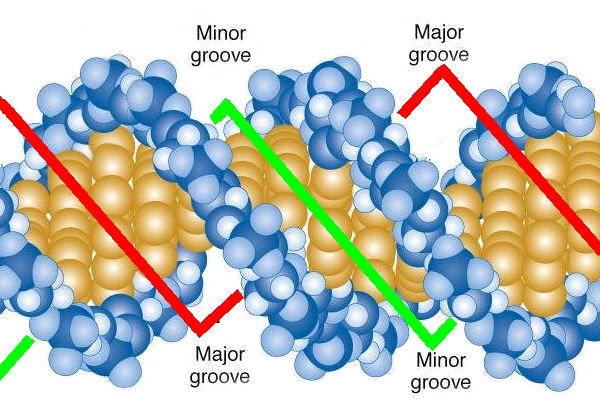
\includegraphics[width=6cm]{major_and_minor_groove_first}}
	\subfloat[]{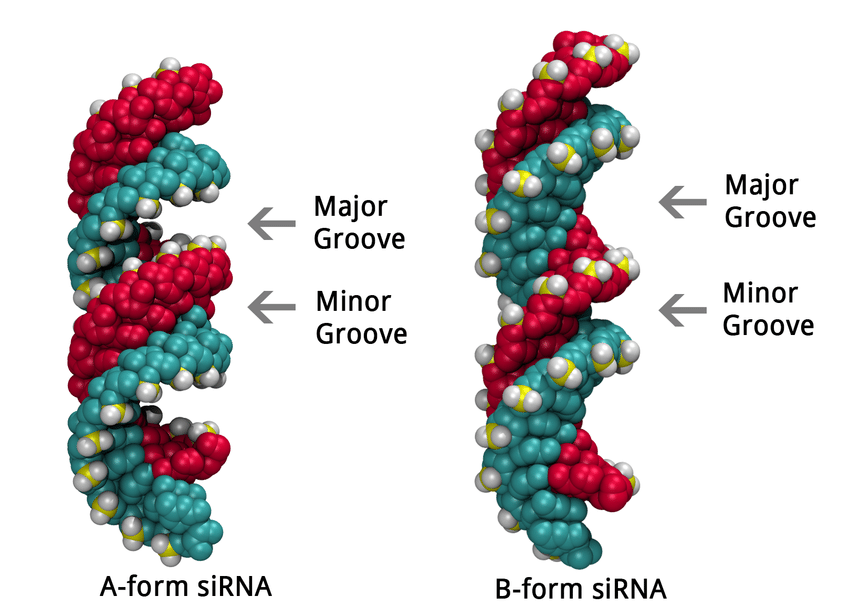
\includegraphics[width=8cm]{major_and_minor_groove_second}}	
	\caption{شیار اصلی و فرعی در مولکول
	\lr{DNA}}
	\label{figure:majorAndMinorGroove}
\end{figure}

فرض کنید که از روی توالی
\lr{ATTA}
پروتئین خاصی ساخته می‌شود و ما می‌خواهیم توالی‌هایی از
\lr{DNA}
که به این صورت است را پیدا کنیم. در چنین موقعی باید به این نکته توجه کنیم که توالی‌های بر روی شیار اصلی و فرعی مهم‌تر هستند و احتمال ساخت پروتئین از روی آنها بیشتر است در نتیجه باید به ساختار سه بعدی مولکول
\lr{DNA}
نیز توجه کنیم. همچنین شیار‌های اصلی در مقایسه با شیار فرعی بیشتر در معرض رونویسی هستند.

\pagebreak
\subsubsection{پکیج کردن مولکول دی ان ای در سلول‌های یوکاریوتی\protect\footnote{\lr{DNA packaging}}}

مجموع طول ماده ژنتیکی هر سلول انسانی حدود دو متر است. حال به این می‌پردازیم که چگونه این موجودی دو متری داخل سلول پنج میکرونی جا شده است به طوری که سلول، جایگاه ژن‌های ضروری را می‌داند.

\begin{figure}[htbp]
	\centering
	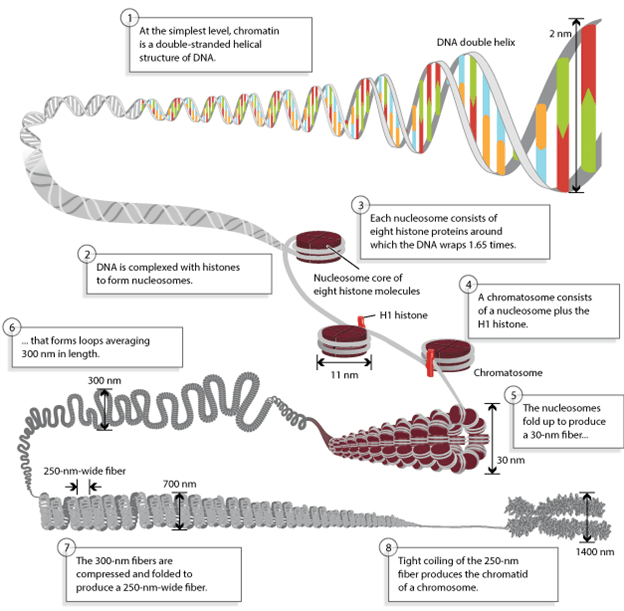
\includegraphics[width = 11cm]{DNA-packaging}
	\caption{پکیج‌کردن مولکول 
	\lr{DNA}}
	\label{figure:dnaPackaging}
\end{figure}

\begin{wrapfigure}[12]{l}{6cm}
	\centering
	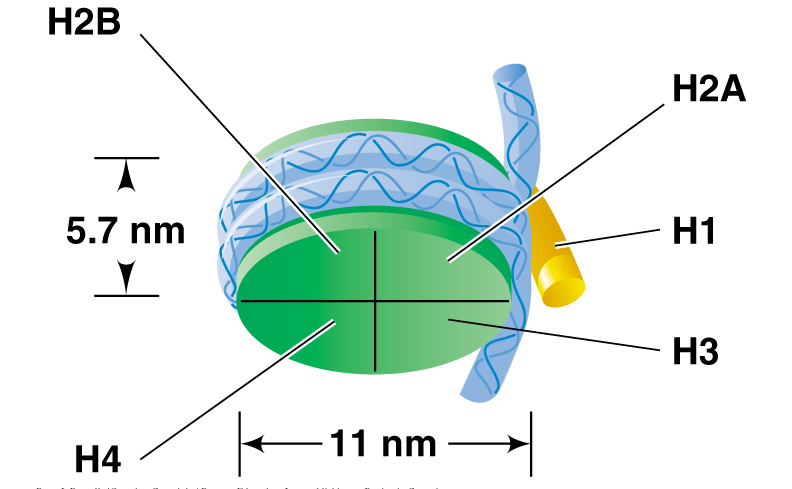
\includegraphics[width=6cm]{Nucleosome}
	\caption{ساختار نوکلئوزوم. از هر کدام از پروتئین‌های نامبرده دو تا کنار هم قرار دارند. 
	\lr{H1}
	جزء نوکلئوزوم نیست.}
	\label{figure:nucleosome}
\end{wrapfigure}


به طور کلی در پکیج کردن مولکول
\lr{DNA}
دو نوع پروتئین به کار میرود:
\begin{itemize}
\item هیستونی
\footnote{\lr{Histones}}
\item غیر هیستونی
\footnote{\lr{Nonhistones}}
\end{itemize}
پروتئین‌های هیستونی بار مثبت دارند و ساختار پایه پکیج کردن یعنی نوکلئوزوم به کمک آن‌ها شکل می‌گیرد.
در مرحله اول هشت مولکول پروتئین در کنار یکدیگر قرار می‌گیرند و سپس رشته
\lr{DNA}
دور آن می‌پیچد به این ساختار یک نوکلئوزوم
\footnote{\lr{Nucleosome}}
گفته می‌شود. نوکلئوزوم به همراه پروتئین
\lr{H1}
کروماتوزوم
\footnote{\lr{Chromatosome}} 
است. تمام پروتئین‌های که در ساختار کروماتوزوم به کار می‌رود هیستونی هستند. همان‌طور که در شکل
\ref{figure:dnaPackaging}
قسمت چهار مشاهده می‌شود به قسمتی از مولکول
\lr{DNA}
که بین دو نوکلئوزوم قرار می‌گیرد
\lr{`Linker'}
گفته می‌شود.
به طور میانگین هر
\lr{Linker}
از 75 جفت باز تشکیل شده است.
در این مرحله قطر ساختار به 11 نانومتر میرسد. 

در مرحله بعد نوکلئوزوم‌ها به کمک پروتئین
\lr{H1}
به هم نزدیک می‌شوند و قطر ساختار را به 30 نانومتر می‌رسانند.

\begin{wrapfigure}[14]{l}{7cm}
	\centering
	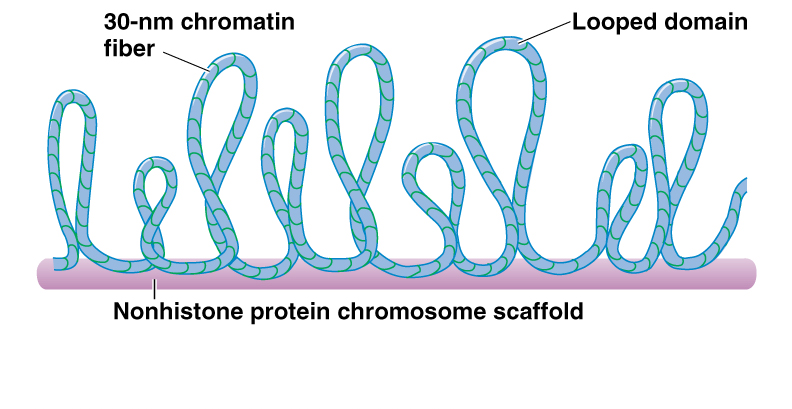
\includegraphics[width=7cm]{DNA-loop}
	\caption{حلقه‌های مولکول 
	\lr{DNA}
	به طول متوسط 300 نانومتر}
	\label{figure:dnaLoop}
\end{wrapfigure}

کروماتینِ 30 نانومتری خم می‌شود و حلقه‌های با طول میانگین 300 نانومتر را می‌سازند. این حلقه‌ها به یک پروتئین غیر هیستونی
(\lr{nonhistone protein scaffolding})
می‌چسبند.

پروتئین‌های غیر هیستونی عموما بار منفی دارند و در نتیجه به سمت پروتئین‌های هیستونی جذب می‌شوند و این در فرآیند پکیج کردن مولکول
\lr{DNA}
مفید است.
پروتئین‌های هیستونی که در مراحل اولیه‌ی پکیج کردن به کار می‌روند دارای تنوع کمی هستند. این تنوع حتی در جانداران متفاوت نیز کم است و طبیعت سعی داشته است با کمترین تغییر‌ آن‌ها را به نسل بعد منتقل کند. اما پروتئین‌های غیر هیستونی که در مراحل انتهایی پکیج کردن به کار می‌روند دارای تنوع بسیار زیادی هستند. هم در جانداران متفاوت فرق دارند و هم در سلول‌های مختلف یک گونه. در واقع همین تفاوت در پروتئین‌های غیر هیستونی است که تفاوت سلول‌ها را بیان می‌کند. همانطور که در شکل
\ref{figure:dnaLoop}
مشخص است نقاطی که در بالای حلقه قرار می‌گیرند احتمال بیشتری برای رونویسی دارند. اینکه کدام قسمت از حلقه در پایین و کدام قسمت در بالا قرار می‌گیرند را پروتئین‌های هیستونی مشخص می‌کنند.

\pagebreak
\subsubsection{همانندسازی دی ان ای\protect\footnote{\lr{DNA replication}}}

در طی تقسیم سلولی نیاز است که مقدار ماده ژنتیکی دو برابر شود و هر رشته
\lr{DNA}
باید همانند خود را بسازد که به این فرآیند، همانندسازی
\lr{DNA}
گفته می‌شود.

 \begin{wrapfigure}{l}{8cm}
	\centering
	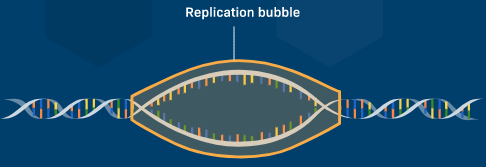
\includegraphics[width=8cm]{Replication_bubble}
	
\includegraphics[width=8cm]{Space}
	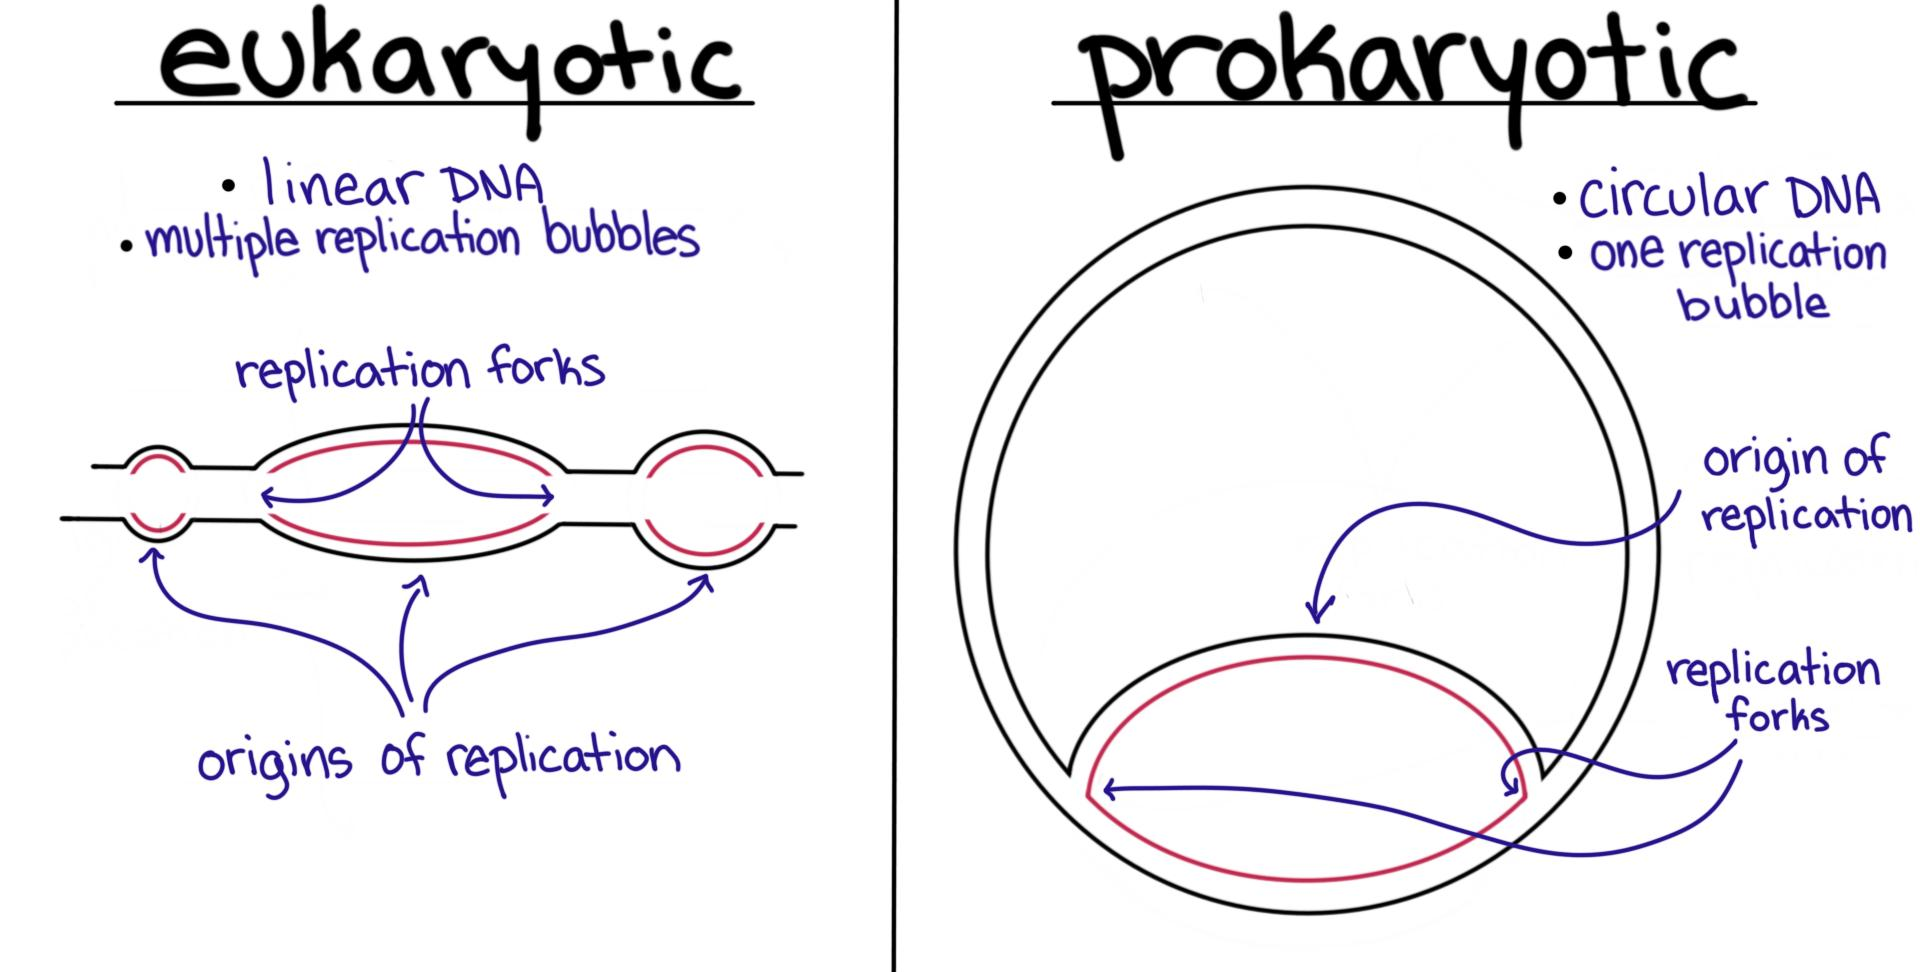
\includegraphics[width=8cm]{cell_eukaryotic_v_prokaryotic_dna_replication}
	\vspace{-20pt}
\end{wrapfigure}

در همانندسازی مولکول
\lr{DNA}
، ابتدا آنزیم هلیکاز
 \footnote{\lr{Helicase}}
 پیوند‌های هیدروژنی را می‌شکند و دو
 \lr{Strand}
 را از هم جدا می‌کند. نقطه‌ای که این گسست شروع می‌شود را 
 \lr{origin point}
 می‌گویند.
 \lr{DNA}
 سلول پروکاریوتی تنها یک
  \lr{origin point}
  دارد اما در سلول یوکاریوتی این نقاط می‌توانند بیشتر باشند و به اصلاح می‌گوید که همانند سازی به صورت موازی
 \footnote{\lr{Parallel}} 
انجام می‌گیرد 
 .
  نقاطی را که هم اکنون در حال باز شدن هستند
  \lr{replication forks}
  می‌نامند.
  
پس از باز شدن رشته توسط آنزیم هلیکاز، آنزیم پرایماز
\footnote{\lr{Primas}}
یک تکه
\lr{RNA}
به یک نخ از رشته
\lr{DNA}
متصل می‌کند که به آن
\lr{RNA primer}
می‌گویند. علت این کار این است که بعد از وصل شد
این قطعه به نخِ رشته
\lr{DNA}
سایر نوکلئوتید‌ها به سمت آن جذب می‌شوند.
  در مرحله بعد به کمک آنزیم
 \lr{DNA}
 پلیمراز
 \RN{3}
 \footnote{\lr{DNA polymerase \RN{3}}}
 نوکلئوتید‌های مکمل که درون غشا قرار دارند در مقابل نخ
 قرار می‌گیرند.
 
 برای فهم کامل همانندسازی باید به ساختار مولکول
 \lr{DNA}
 توجه کنیم. همانطور که قبلا گفته شد دو رشته مولکول
 \lr{DNA}
 به صورت
 \lr{antiparallel}
 در مقابل همدیگر قرار می‌گیرند به این معنی که یکی در جهت
$ 5^\prime $
  به
$ 3^\prime $
  است و دیگری در جهت
$ 3^\prime $
  به
$ 5^\prime $
.
و اما نکته‌ای که وجود دارد این است که آنزیم
\lr{DNA}
پلیمراز
تنها در جهت
$ 3^\prime $
  به
$ 5^\prime $
می‌تواند حرکت کند چرا که ساخت پروتئین تنها در جهت
$ 5^\prime $
  به
$ 3^\prime $
انجام می‌شود
.
شکل
\ref{figure:dnaReplication}
را مشاهده کنید.
در نتیجه این آنزیم ابتدا روی یکی از رشته‌ها که به آن
\lr{leading strand}
گفته می‌شود، حرکت می‌کند. برای رشته مقابل یعنی
\lr{lagging strand}
از سمت
\lr{replication fork}
به سمت
\lr{origin point}
حرکت می‌کند.
همانندسازی
\lr{leading strand}
به صورت پیوسته است اما در
\lr{lagging strand}
،
\lr{DNA}
پلیمراز
مجبور است همانندسازی را در قطعه‌هایی به اسم
\lr{Okazaki fragment}
انجام دهد. توجه کنید که در
\lr{lagging strand}
به ازای هر
\lr{Okazaki fragment}
ابتدا آنزیم
\lr{Primase}
یک
\lr{RNA Primer}
بر روی نخِ رشته قرار می‌دهد.  اما در
\lr{leading strand}
تنها یک
\lr{RNA Primer}
کافی است.


\begin{figure}[htbp]
	\centering
	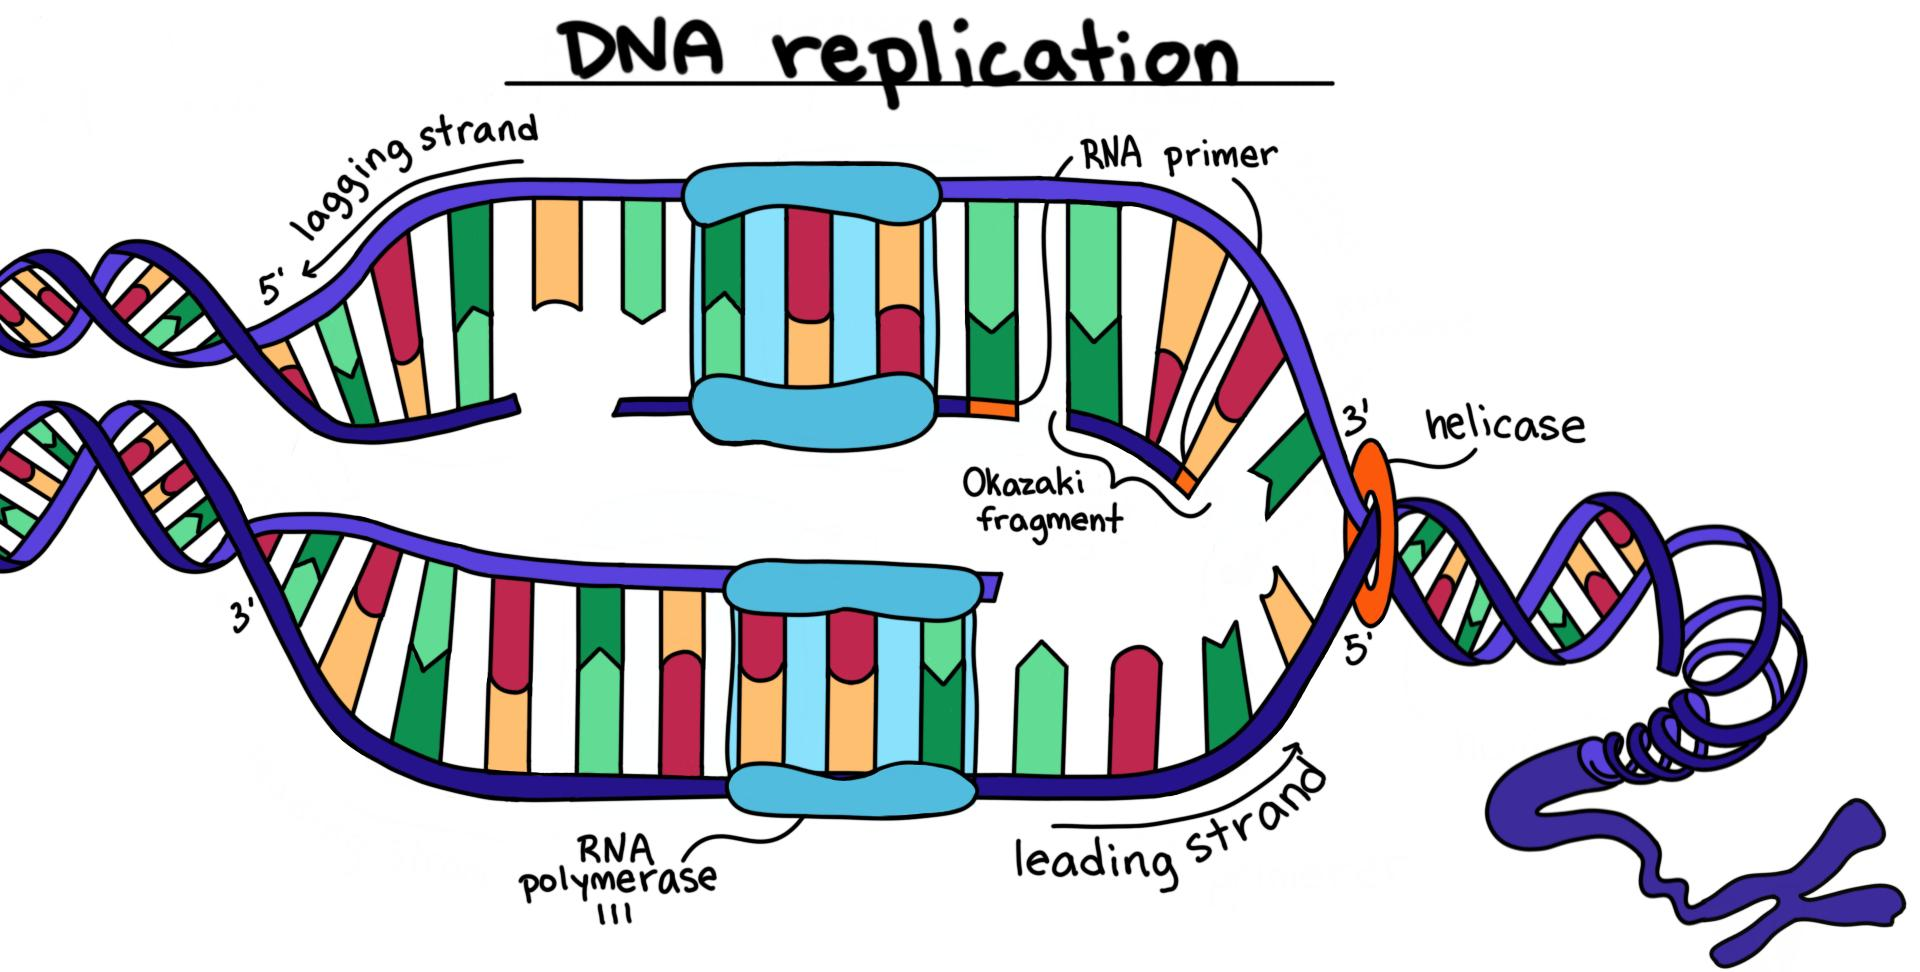
\includegraphics[width=10cm]{dna_replication_eukaryotic}
	\caption{همانندسازی 
	\lr{DNA}
	به کمک دو آنزیم هلیکاز و  
	\lr{DNA} 
	پلیمراز
	در سلول یوکاریوتی
	}
	\label{figure:dnaReplication}
\end{figure}

\pagebreak
\begin{wrapfigure}{l}{8cm}
	\centering
	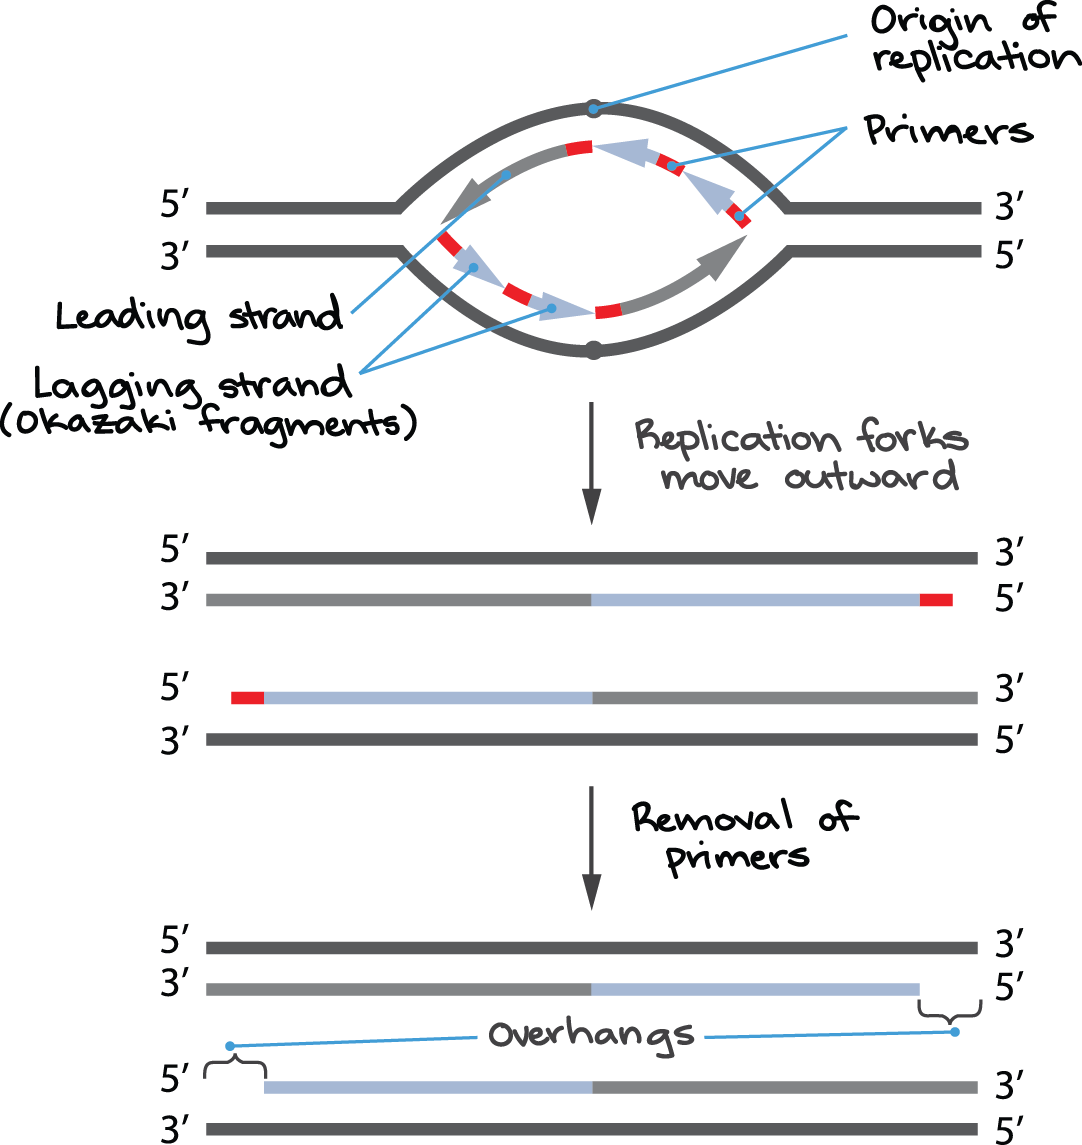
\includegraphics[width=8cm]{Worn_off_of_telomeres}
\end{wrapfigure}

\begin{figure}[htbp]
	\centering
	\subfloat[]{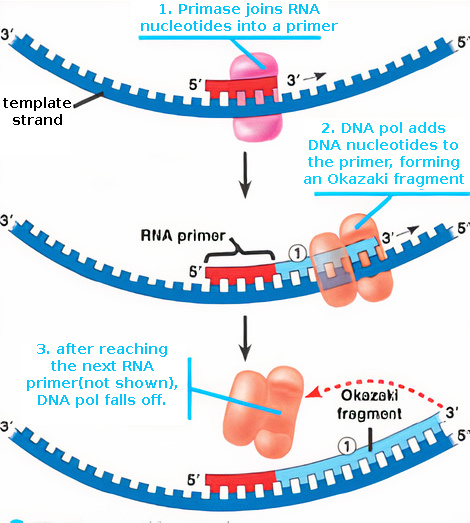
\includegraphics[width=6.5cm]{Replication_one}}
	\hspace{20pt}	
	\subfloat[]{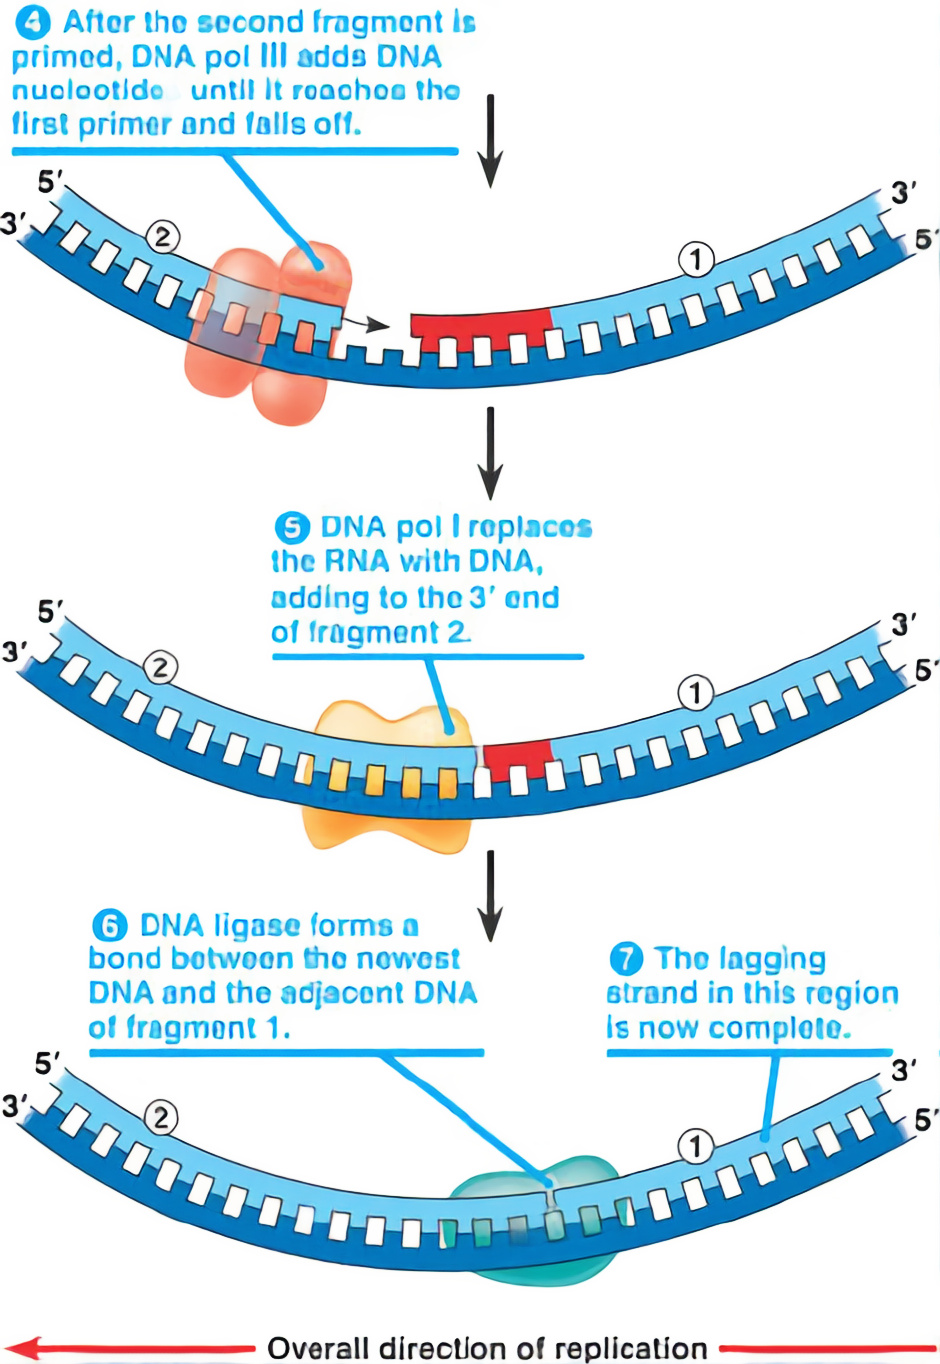
\includegraphics[width=6.5cm]{Replication_two}}
	\caption{مراحل همانندسازی دی ان ای}
	\label{figure:replication_sections}
\end{figure}

بعد از انجام همانند سازی توسط
 \lr{DNA}
 پلیمراز
 \RN{3}
 نیاز است که
 \lr{RNA Primer}
 ها حذف شوند و جای آن‌ها نخِ
 \lr{DNA}
 قرار گیرد.  در
\lr{lagging strand}
 بعد از تمام شدن هر
\lr{Okazaki fragment}
،
\lr{DNA}
پلیمراز
\RN{1}
،
\lr{RNA primer}
ای که مربوط به
\lr{Okazaki fragment}
قبلی است را با
\lr{DNA}
جایگزین می‌کند. سپس آنزیم
\lr{DNA}
لیگاز
\footnote{\lr{DNA ligase}}
پیوند بین دو تکه رشته
\lr{DNA}
را برقرار می‌کند.
به شکل
\ref{figure:replication_sections}
توجه کنید.
در سلول‌های پروکاریوتی نیز با توجه به اینکه کروموزوم حلقوی دارند، بعد از اتمام همانندسازی در یک جهت
\lr{DNA}
پلیمراز
\RN{3}
به
\lr{RNA primer}
می‌رسد و در نتیجه
\lr{DNA}
پلیمراز
\RN{3}
رشته را رها می‌کند و
\lr{DNA}
پلیمراز
\RN{1}
،
\lr{RNA primer}
را با
\lr{DNA}
جایگزین می‌کند.
در سلول‌های یوکاریوتی جایگاه اولین پرایماز در انتهای کروموزوم توسط
\lr{DNA}
پلیمراز
\RN{3}
تشخیص داده نمی‌شود در نتیجه این قسمت از
\lr{DNA}
از بین می‌رود و در نتیجه در هربار انجام همانندسازی مقدار کمی از دم کروموزوم از بین می‌رود.
برای جلوگیری از بین رفتن ژن‌ها کروموزوم یوکاریوتی قسمتی به اسم
تلومر
\footnote{\lr{telomeres}}
دارد. در واقع تلومر در دو سر کروموزوم قرار دارد. تلومر از تکرار صدها یا هزاران بارِ یک دنباله کوتاه
\lr{DNA}
تشکیل شده است. این دنباله در جانداران مختلف فرق دارد اما در انسان و سایر پستانداران به صورت
$ 5^\prime-TTAGGG-3^\prime $
است.
تلومر عمر انسان را مشخص می‌کند چرا که با کوتاه شدن تلومر ژن‌های حساس نیز از بین می‌روند و عملکرد سلول مختل می‌شود. در واقع به همین خاطر است که سلول تعداد محدودی تقسیم انجام می‌دهد.

\begin{wrapfigure}[14]{l}{9cm}
	\centering
	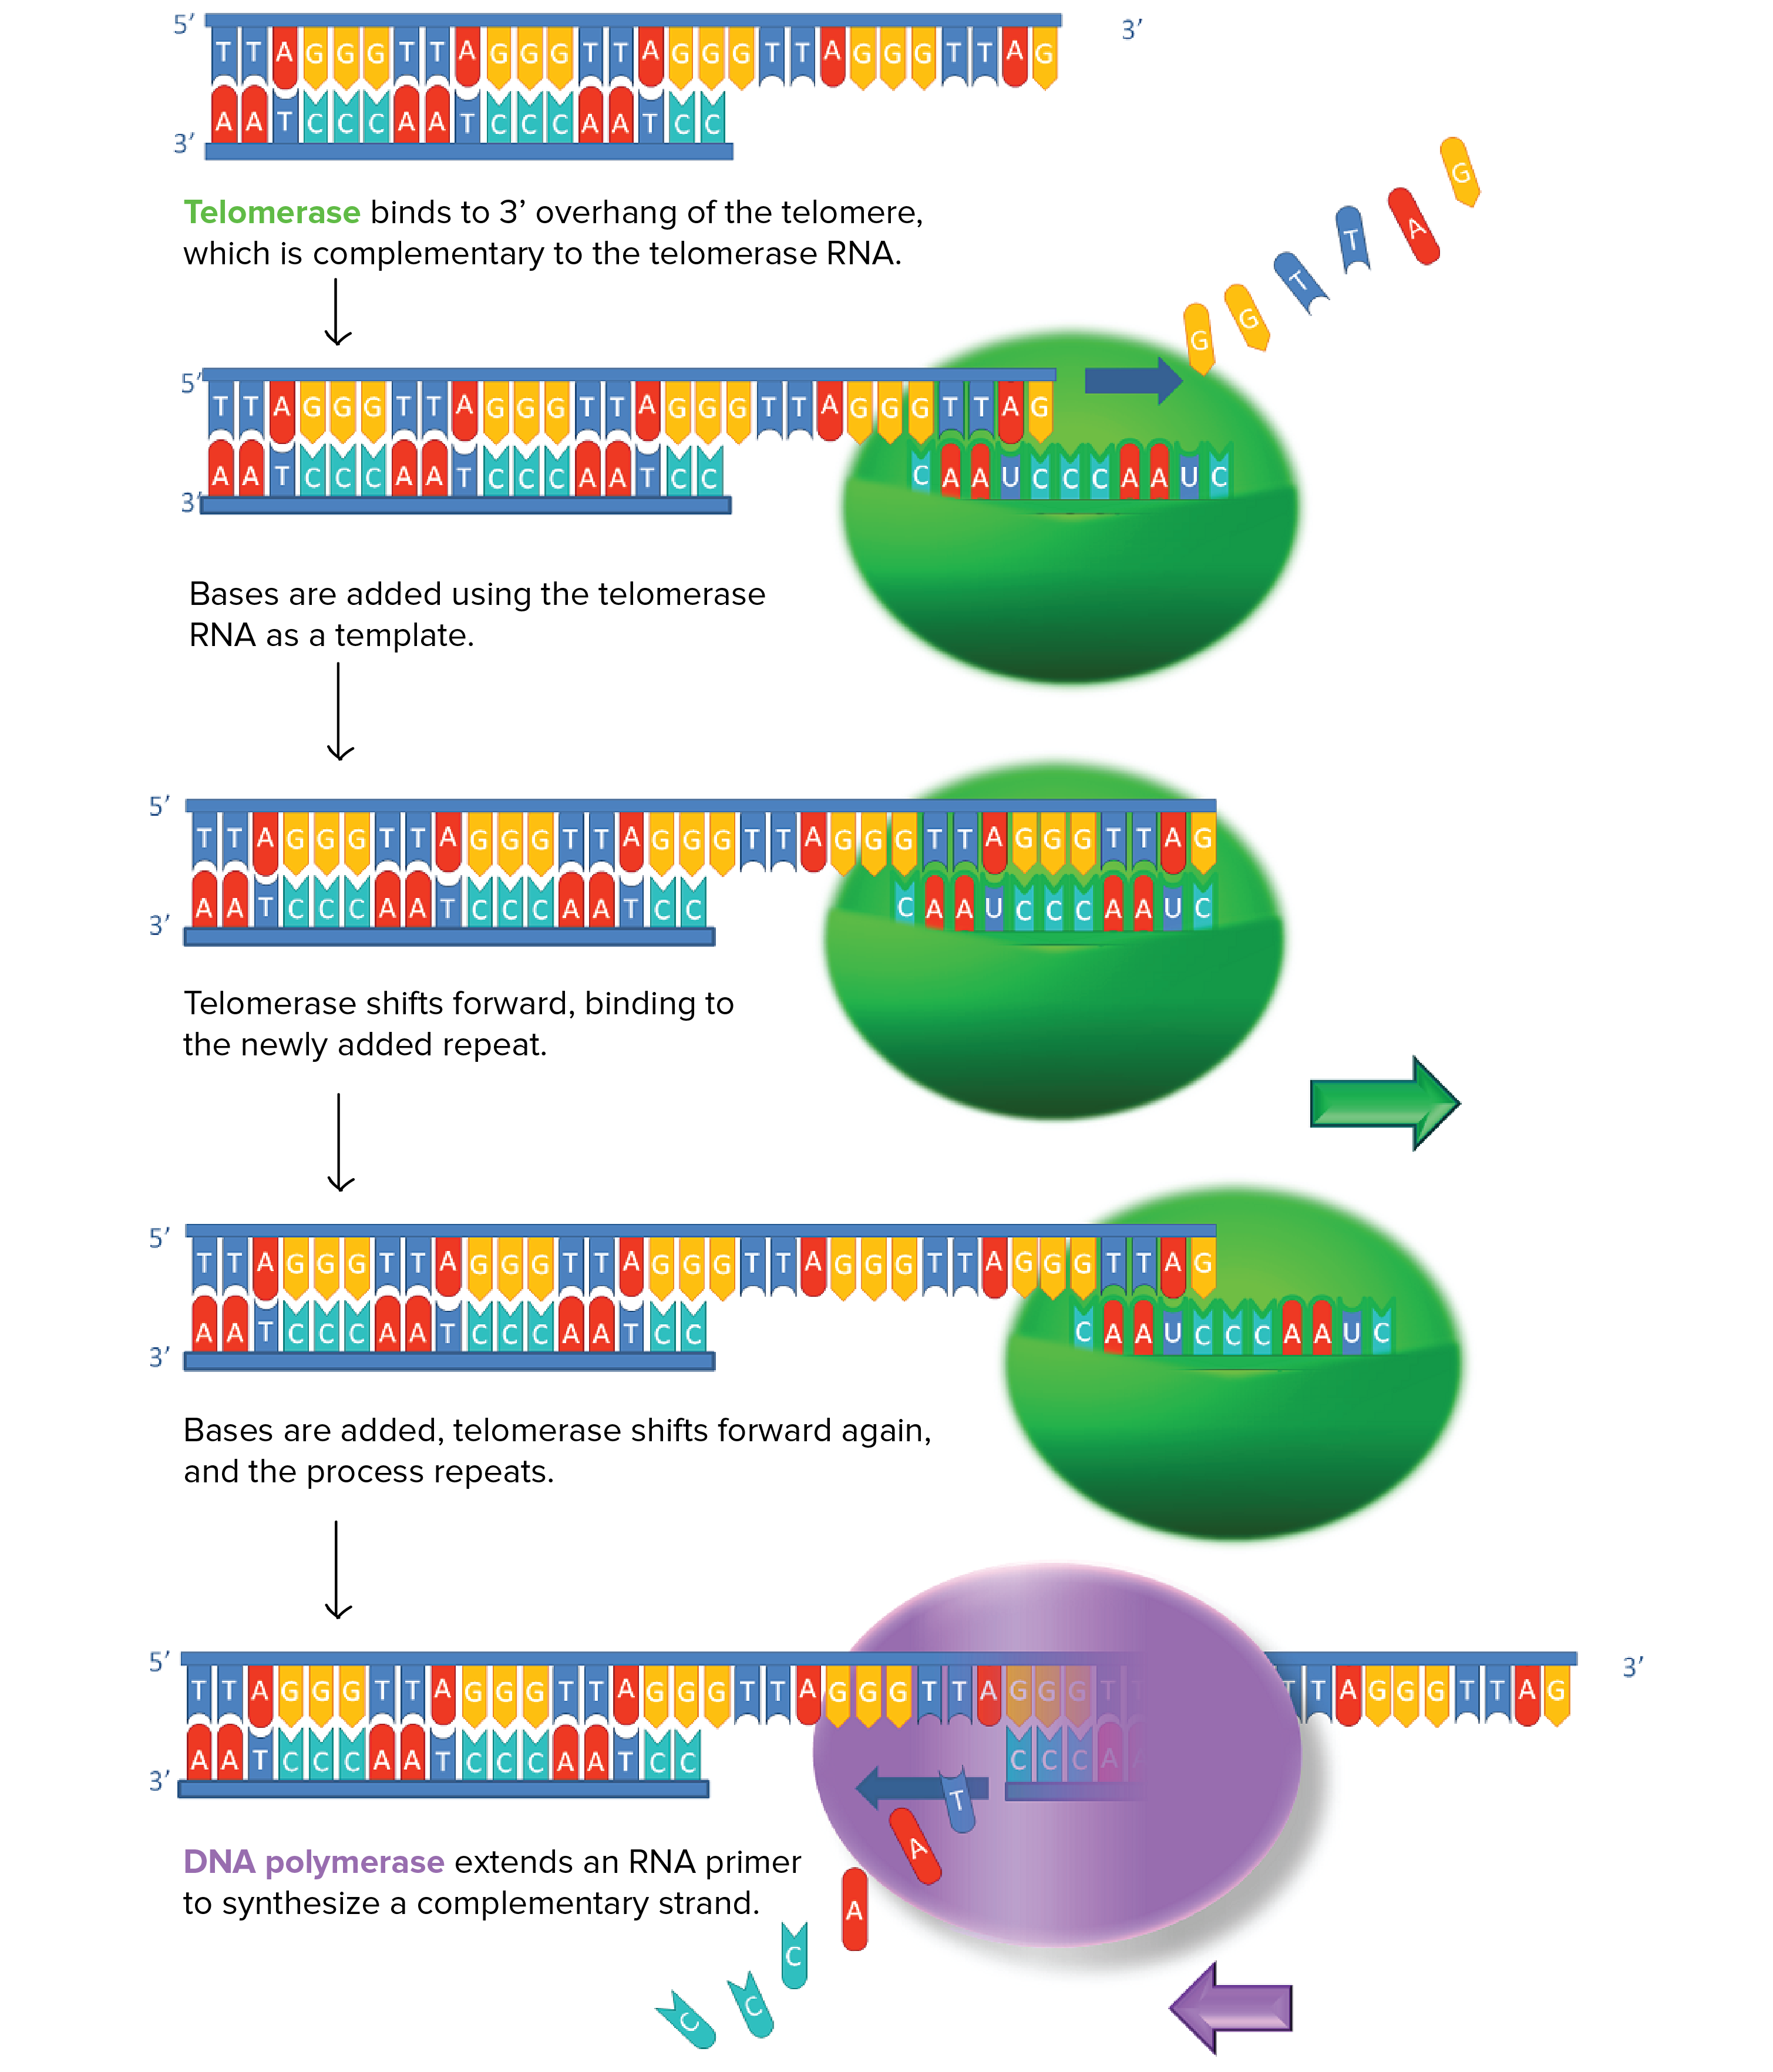
\includegraphics[width=9cm]{Telomerase_function}
	\caption{ انزیم تلومراز از کوتاه شدن 
	\lr{DNA}
	در سلول‌های جنسی جلوگیری می‌کند.}
	\label{figure:TelomeraseFunction}
\end{wrapfigure}

نکته‌ای که وجود دارد این است که اگر این کوتاه شدن تلومر در سلول‌های جنسی نیز اتفاق بیافتد، نسل به نسل ماده ژنتیک کوتاه می‌شود و در نتیجه گونه منقرض می‌شود. به همین علت آنزیمی به اسم تلومراز
\footnote{\lr{Telomerase}}
یک تکه اضافه به انتهای کروموزوم اضافه می‌کند.
در شکل
\ref{figure:TelomeraseFunction}
نحوه عملکرد این آنزیم نشان داده شده است.

در رشته جدید ایجاد شده یک
\lr{Strand}
از رشته قبلی گرفته شده و یک
\lr{Strand}
توسط آنزیم 
\lr{DNA}
پلیمراز ساخته شده است به همین علت گفته می‌شود که همانندسازی
\lr{DNA}
به صورت نیمه حفظ شده
\footnote{\lr{Semi conservative}}
 است.

آنزیم
\lr{DNA}
پلیمراز عمل دیگری نیز انجام می‌دهد که ویرایش
\footnote{\lr{proofriding}}
نام دارد. طی ویرایش آنزیم روی رشته حرکت می‌کند و اگر نوکلئوتیدی به اشتباه در رشته قرار گرفته باشد با نوکلئوتید درست جایگزین می‌کند.

\pagebreak
\subsubsection{آغاز همانندسازی دی ان ای در ای کولای\protect\footnote{\lr{E. coli}}}

همانندسازی دی ان ای در ای کولای سه مرحله دارد:
\begin{itemize}
\item \lr{chain initiation}
\item \lr{chain extension}
\item \lr{chain termination}
\end{itemize}

باکتری
\lr{E. coli}
دارای یک کروموزوم حلقوی است. این کروموزوم حلقوی دارای دنباله‌ای کوتاه از نوکلئوتید‌ها است که
\lr{replication origin (oriC)}
نام دارد.
\lr{oriC}
مخفف
\lr{\textcolor{red}{Ori}gin of \textcolor{red}{C}hromosomal}
است.
\lr{oriC}
دارای 245 جفت‌باز است که نسبت به سایر باکتری‌ها به شدت محافظت می‌شود.

\lr{oriC}
دارای چند نوع ناحیه مهم است که در شروع همانند‌سازی اهمیت دارند:

\begin{description}
\item[\lr{R sites}]
\lr{oriC}
دارای 5 جایگاه
\lr{R}
است که هر کدام از 9 جفت نوکلئوتید تشکیل شده‌اند.  این 5 جایگاه یک
\lr{binding site}
برای پروتئین آغاز کننده یعنی
\lr{DnaA}
ایجاد می‌کنند.
\item[\lr{I sites}]
این جایگاه‌ها نیز میزبان
\lr{DnaA}
هستند.
\item[\lr{DNA unwinding element (DUE)}]
دنباله‌ای از سه بار تکرار 13 جفت‌باز است که جفت‌باز‌های
\lr{A--T}
در آن زیاد است. با توجه به اینکه بین باز آدنین و تیمین دو پیوند هیدروژنی برقرار می‌شود وقتی ناحیه غنی از این جفت‌باز باشد نسبتا سست‌تر است و آسان‌تر گسسته می‌شود.
\item[\lr{binding site for the protein IHF}]
(
\lr{IHF}
مخفف
عامل میزبان ادغام
\footnote{\lr{integration host factor}}
است.
)
\item[\lr{binding site for the protein FIS}]
(
\lr{FIS}
مخفف
عامل تحریک وارونگی
\footnote{\lr{factor for inversion stimulation}}
است.
)
\item[\lr{GATC methylation sites}]
جایگاه‌هایی برای گروه متیل
\end{description}

\begin{figure}[htbp]
	\centering
	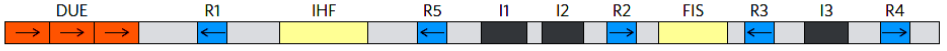
\includegraphics[width=10cm]{Ecoli_elememts_of_oric}
\end{figure}

\begin{figure}[htbp]
	\centering
	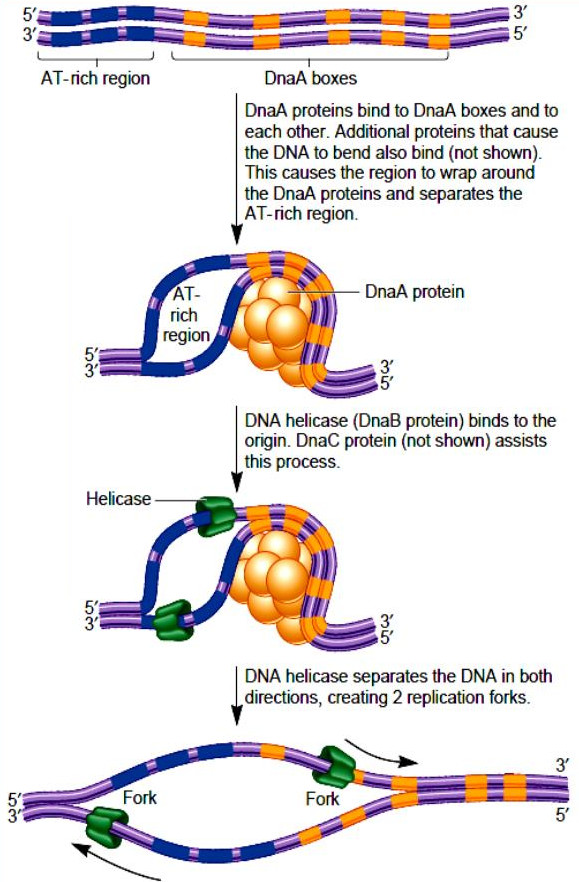
\includegraphics[width=7cm]{Ecoli_replication_origin}
	\caption{آغاز همانندسازی در ای کولای}
	\label{figure:ecoliInitialReproduction}
\end{figure}

\begin{wrapfigure}{l}{6cm}
	\centering
	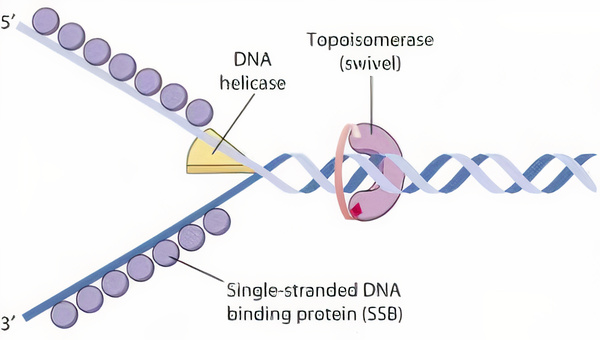
\includegraphics[width=6cm]{Single_stranded_binding_proteins}
	\caption{\lr{Single stranded binding proteins and topoisomerase}}
	\label{figure:SingleStrandedBindingProteins}
\end{wrapfigure}

همانطور که در شکل
\ref{figure:ecoliInitialReproduction}
مشخص است پروتئین
\lr{DnaA}
به همراه چند پروتئین دیگر
به
\lr{DnaA box}
ها میچسبد و این باعث می‌شود تا
\lr{AT-rich region}
باز شود سپس دو آنزیم هلیکاز به دو سمت این
\lr{Replication bubble}
می‌چسبند و شروع به باز کردن بیشتر این ناحیه می‌کنند.

همانطور که در شکل
\ref{figure:SingleStrandedBindingProteins}
مشاهده می‌کنید با حرکت هلیکاز به سمت جلو دو اتفاق می‌افتد اول اینکه ممکن است رشته پشت سر آن دوباره به هم بچسبد به همین خاطر پروتئین‌هایی به نام
\lr{Single Stranded Binding Protein}
به دو نخِ رشته
\lr{DNA}
پیچسبند تا فرصت برای همانندسازی این قسمت فراهم شود. دوم اینکه با حرکت هلیکاز به سمت جلو رشته
\lr{DNA}
در جلو آن فشرده می‌شود به همین خاطر
\lr{Topoisomerase}
رشته
\lr{DNA}
را می‌چرخاند تا فشردگی آن کم شود یا به اصطلاح از
\lr{over winding}
جلوگیری می‌کند.

\begin{figure}[htbp]
	\centering
	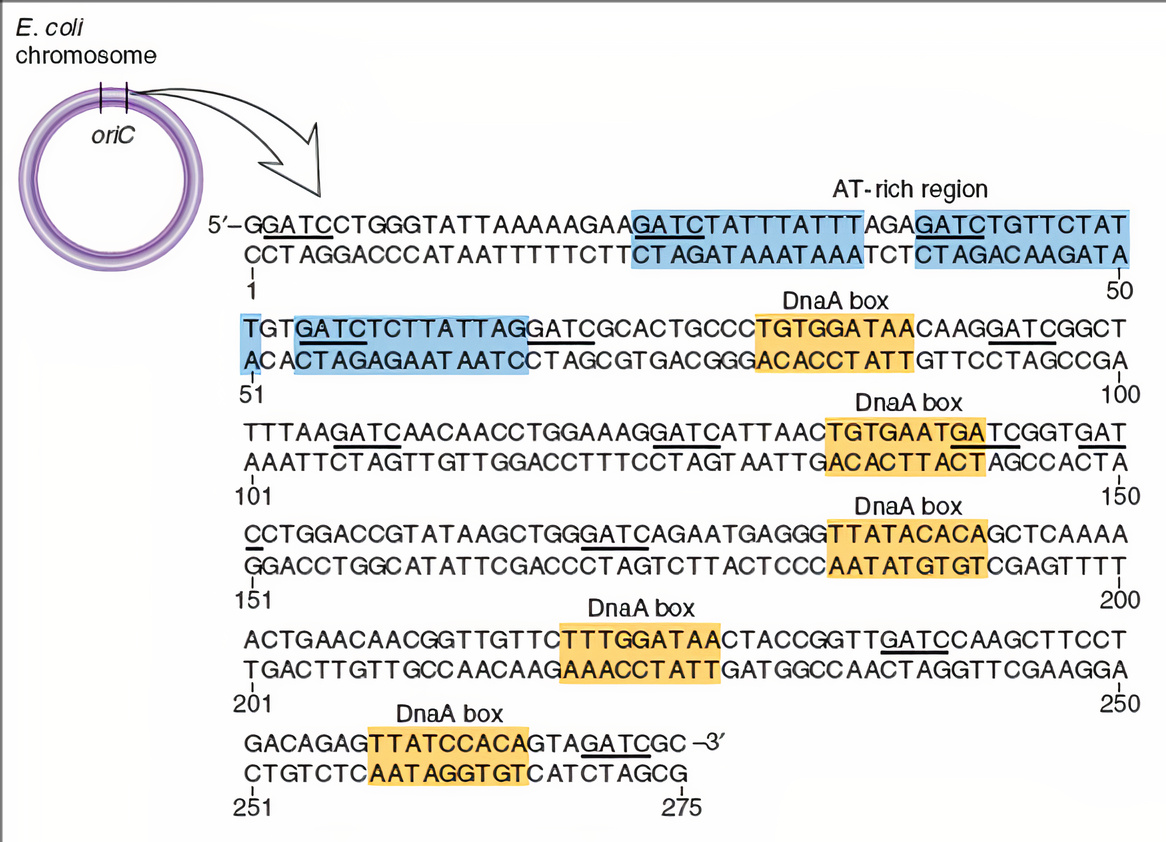
\includegraphics[width=8cm]{ecoli_oric_sequence}
\end{figure}

\pagebreak
\subsubsection{تقسیم دوتایی در باکتری‌ها\protect\footnote{\lr{Binary fission}}}

\begin{wrapfigure}[15]{l}{10cm}
	\centering
	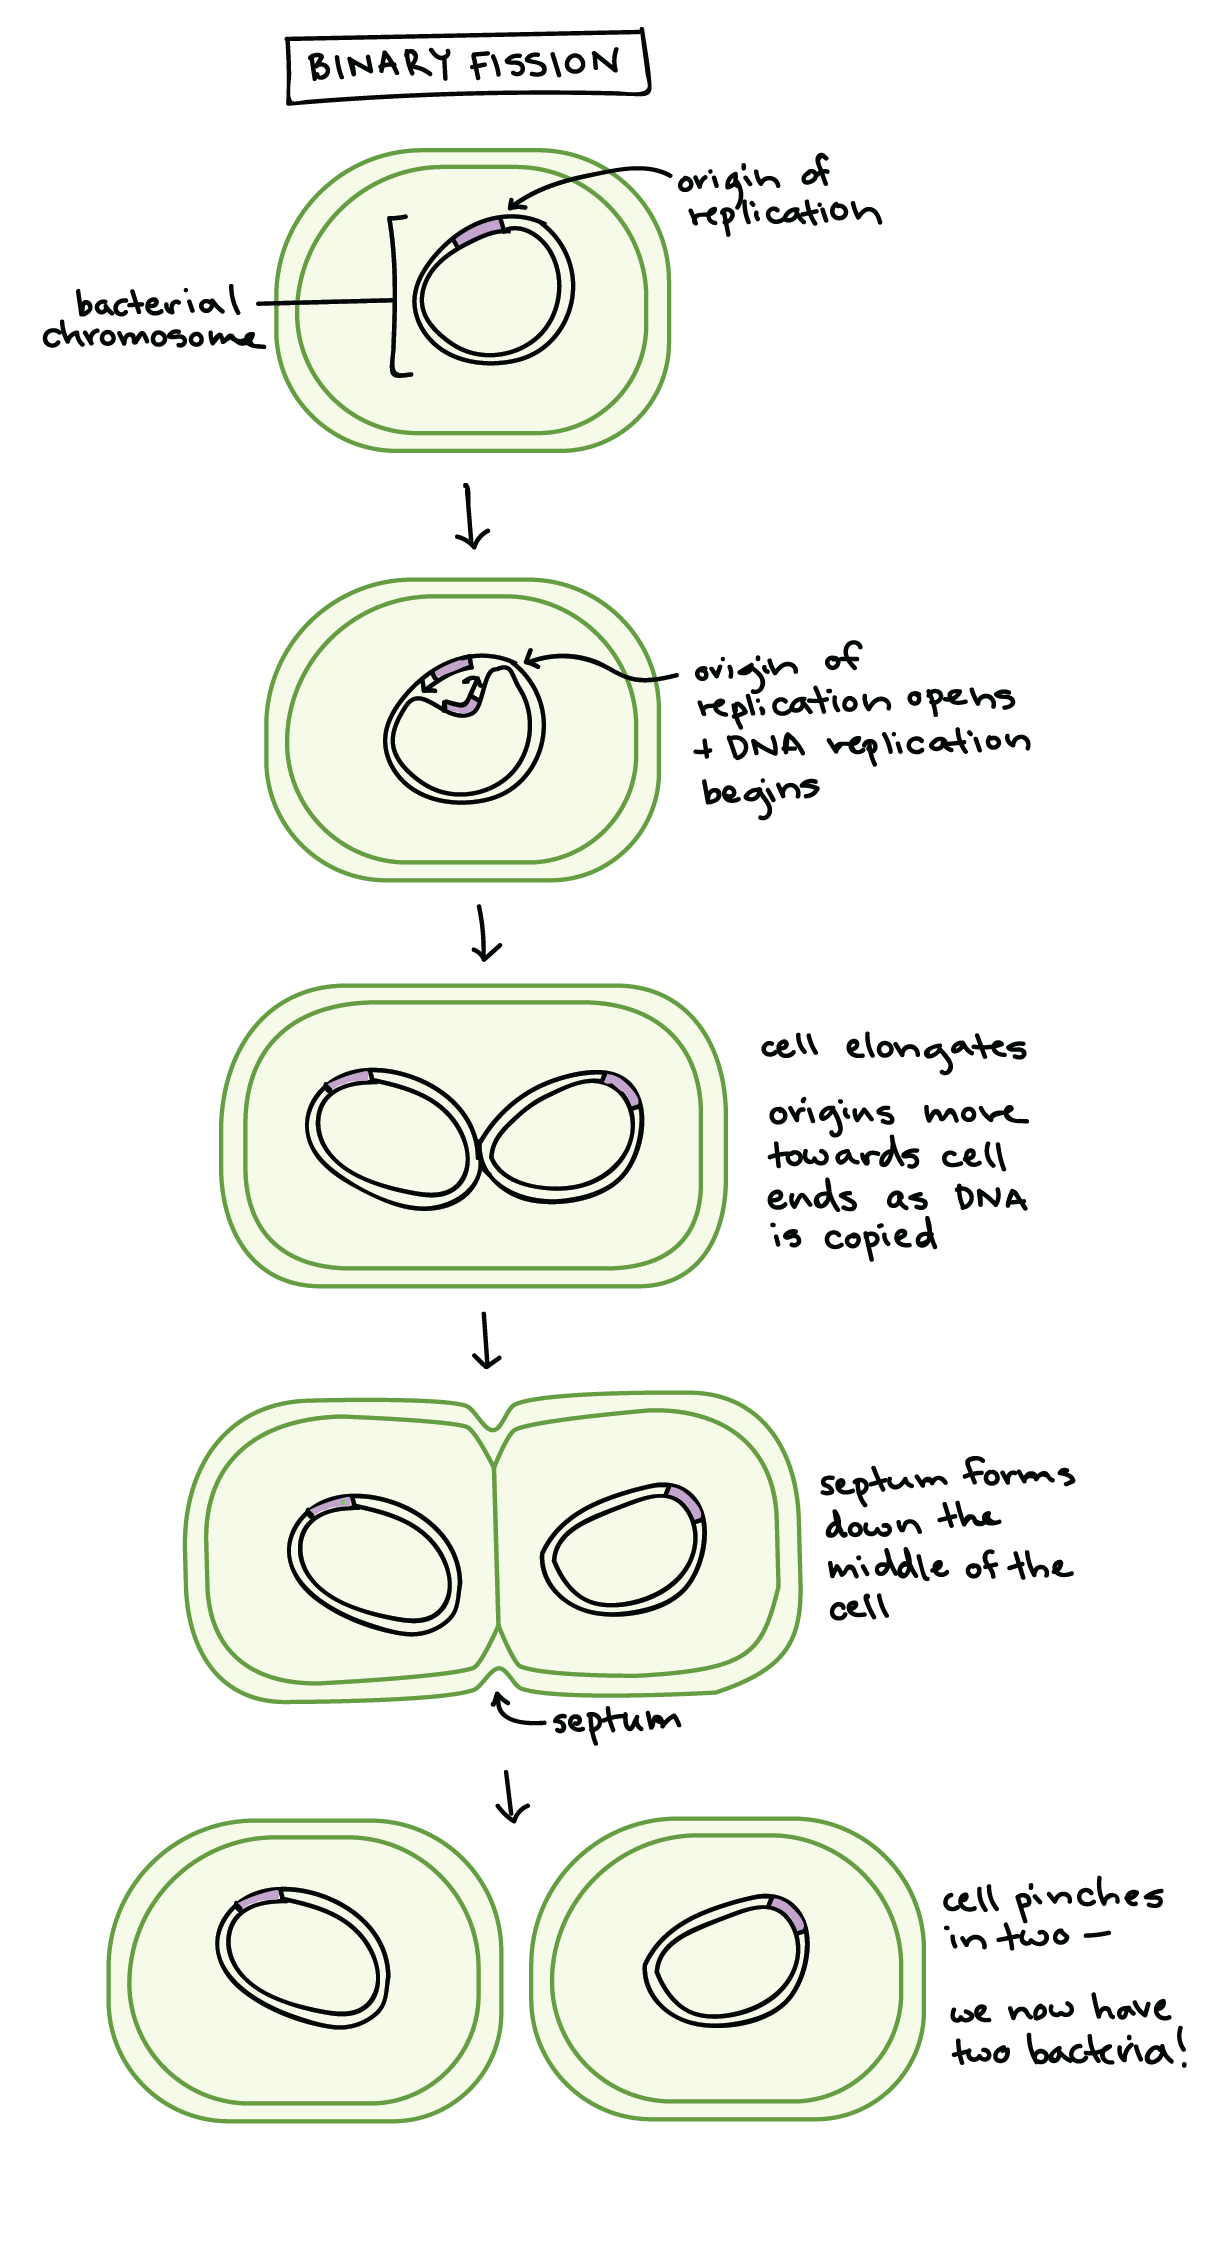
\includegraphics[width=10cm]{Binary_fission}
\end{wrapfigure}

تقسیم سلولی در جاندارانی مثل باکتری‌ها ساده‌تر از تقسیم سلولی در یوکاریوت‌ها است. باکتری‌ها دارای
\lr{DNA}
حلقوی هستند و به روش تقسیم دوتایی تکثیر پیدا می‌کنند. تنها علت برای تقسیم سلولی در باکتری‌ها تولیدمثل است.

باکتری‌ها برخلاف سلول‌های یوکاریوتی اغلب تنها یک کروموزوم حلقوی دارند. و هیچگاه هسته ندارند با این حال کروموزوم آنها درون ناحیه‌ای به نام نوکلئوید
\footnote{\lr{Nulceoid}}
قرار دارد.

تقسیم دوتایی با همانندسازی
\lr{DNA}
آغاز می‌شود. در
\lr{DNA}
حلقوی تنها یک
\lr{origin point}
وجود دارد و همانندسازی انقدر ادامه پیدا می‌کند تا در نقطه مقابل به هم برسد. طی این همانندسازی
\lr{origine point}
ها به سمت مخالف می‌روند و به همراه خود کروموزوم‌ها را نیز می‌کشند.

\pagebreak
\subsubsection{تقسیم سلولی میتوز}
همه سلول‌های یوکاریوتی دارای یک چرخه زندگی
\footnote{\lr{Cell cycle}}
 هستند که طی آن رشد می‌کنند و سپس تقسیم می‌شوند و دو سلول دختری می‌سازند.

\begin{wrapfigure}[12]{l}{7cm}
	\centering
	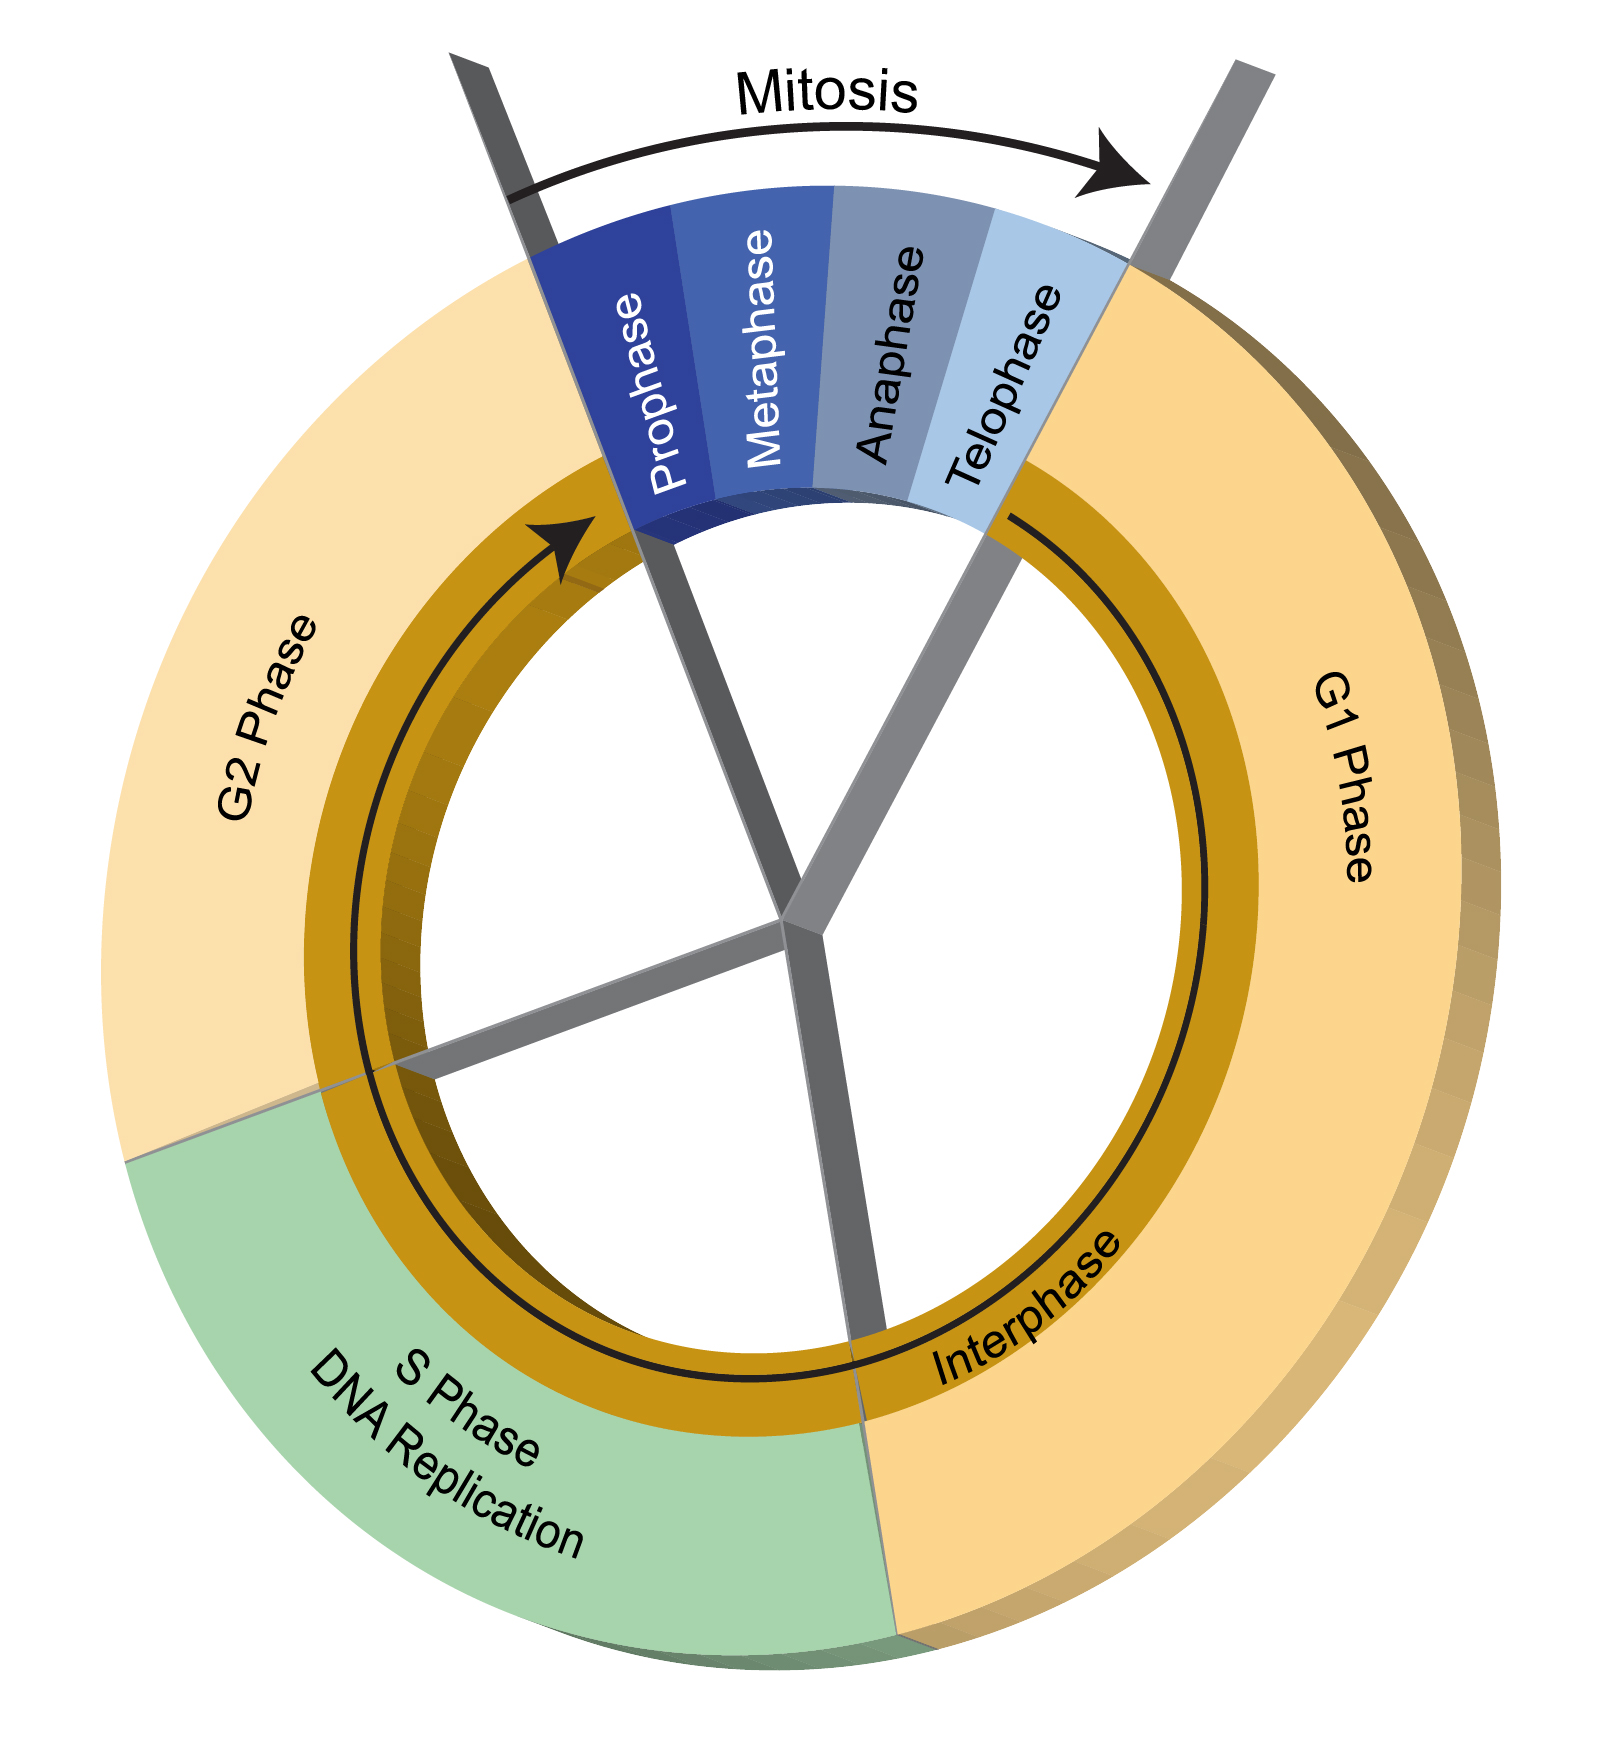
\includegraphics[width=7cm]{Cell_cycle}
	\caption{ چرخه زندگی سلول}
	\label{figure:cellCycle}
\end{wrapfigure}

چرخه زندگی سلول دارای دو بخش اصلی است:
\begin{itemize}
\item اینترفاز
\footnote{\lr{Interphase}}
که طی آن سلول رشد می‌کند و آماده تقسیم می‌شود.
\item میتوتیک فاز
\footnote{\lr{Mitotic (M) phase}}
که طی آن سلول تقسیم می‌شود.
\end{itemize}

اینترفاز خود شامل سه مرحله است:
\begin{description}
\item[\lr{$ G_{1} $ Phase}]
طی این مرحله سلول رشد می‌کند و بزرگ می‌شود.
\item[\lr{$ S $ Phase}]
در این مرحله همانندسازی
\lr{DNA}
رخ می‌دهد.
\item[\lr{$ G_{2} $ Phase}]
طی این مرحله نیز سلول رشد می‌کند. همچنین اندامک‌های لازم همانندسازی می‌کنند و شرایط برای تقسیم سلولی مهیا می‌شود.
\end{description}

میتوتیک فاز نیز خود از دو مرحله تشکیل شده است:
\begin{itemize}
\item میتوز
\footnote{\lr{Mitosis}}
\item سیتوکینز
\footnote{\lr{Cytokinesis}}
\end{itemize}

\bigskip
\bigskip
\bigskip
میتوز خود از چهار مرحله تشکیل شده است:

\begin{figure}[h]
	\centering 
	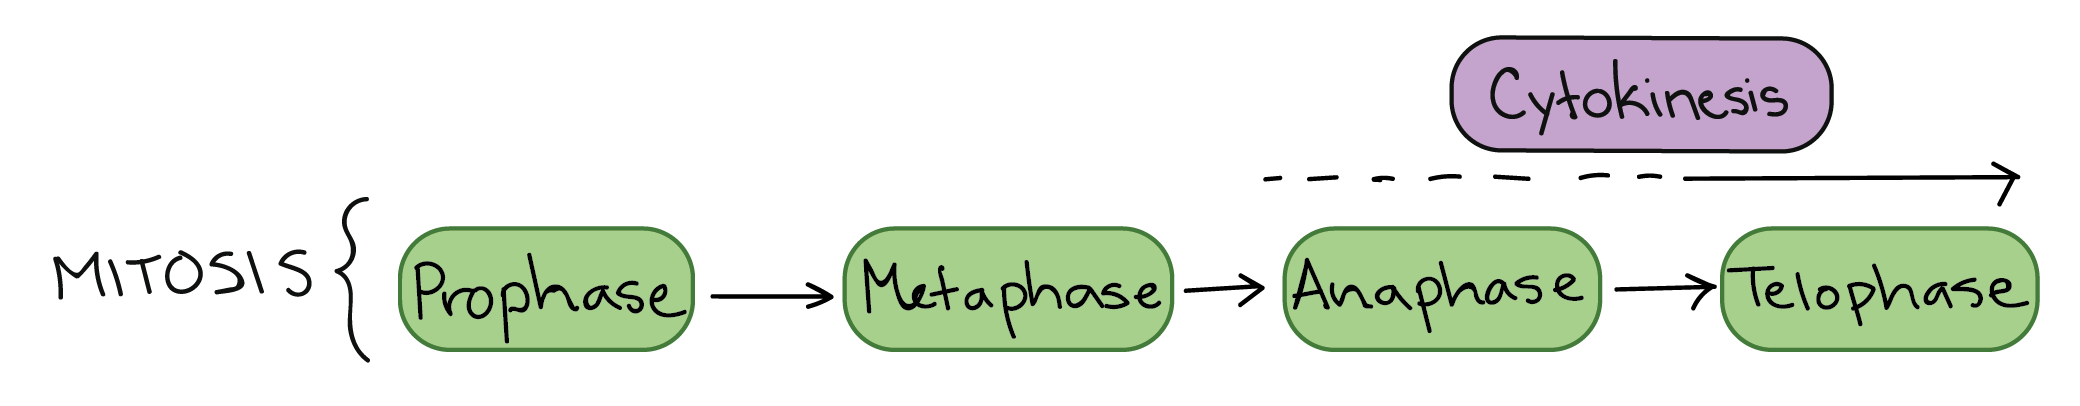
\includegraphics[width=10cm]{Steps_of_mitosis}
\end{figure}

\begin{description}
\item[\lr{Prophase}]
در این مرحله رشته‌های کروماتینی ضخیم، کوتاه و قابل رؤیت می‌شوند. پوشش هسته ناپدید می‌شود و با دور شدن سانتریول‌ها از یکدیگر دوک شکل می‌گیرد.

\begin{figure}[h]
	\centering
	\subfloat[]{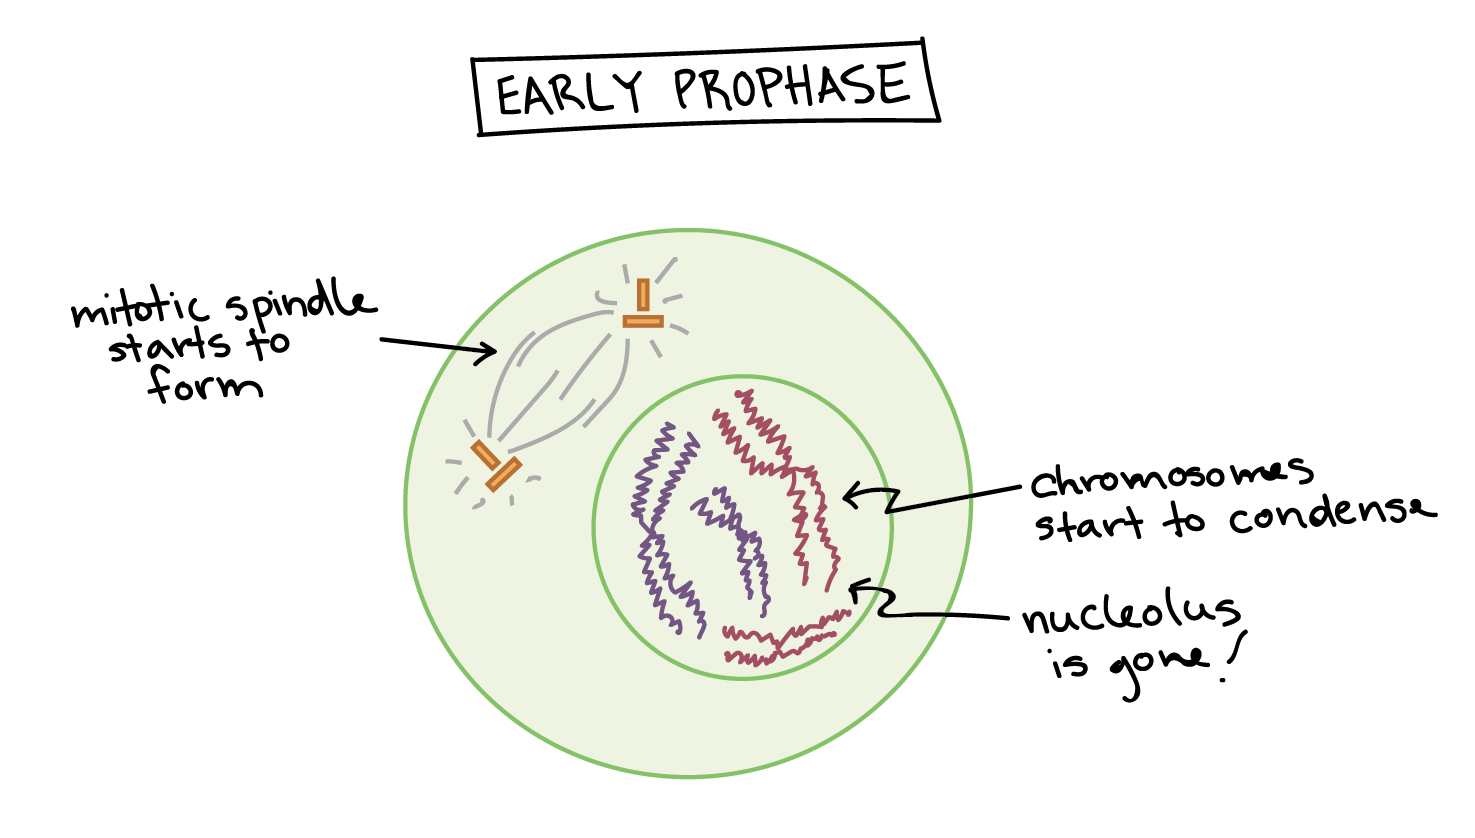
\includegraphics[width=7cm]{Early_prophase}}
	\subfloat[]{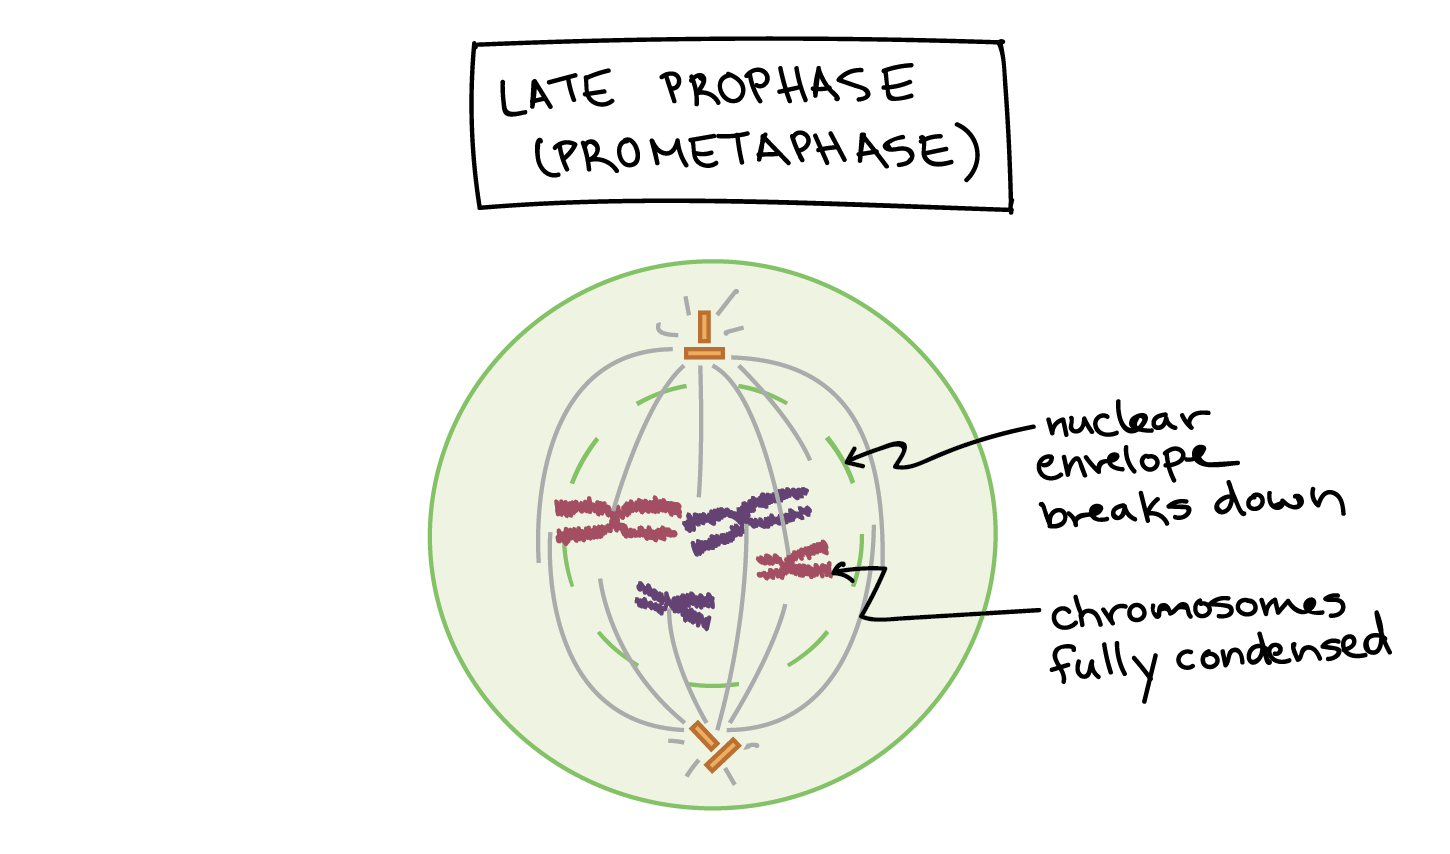
\includegraphics[width=7cm]{Late_prophase}}
\end{figure}

\pagebreak
\item[\lr{Metaphase}]
متا به معنی وسط است.
در متافاز کروموزوم‌ها به سمت وسط سلول حرکت می‌کنند و در سطح استوایی سلول ردیف می‌شوند. در متافاز دو کروماتید هر کروموزوم حداکثر فشردگی را دارند.

\begin{figure}[h]
	\centering
	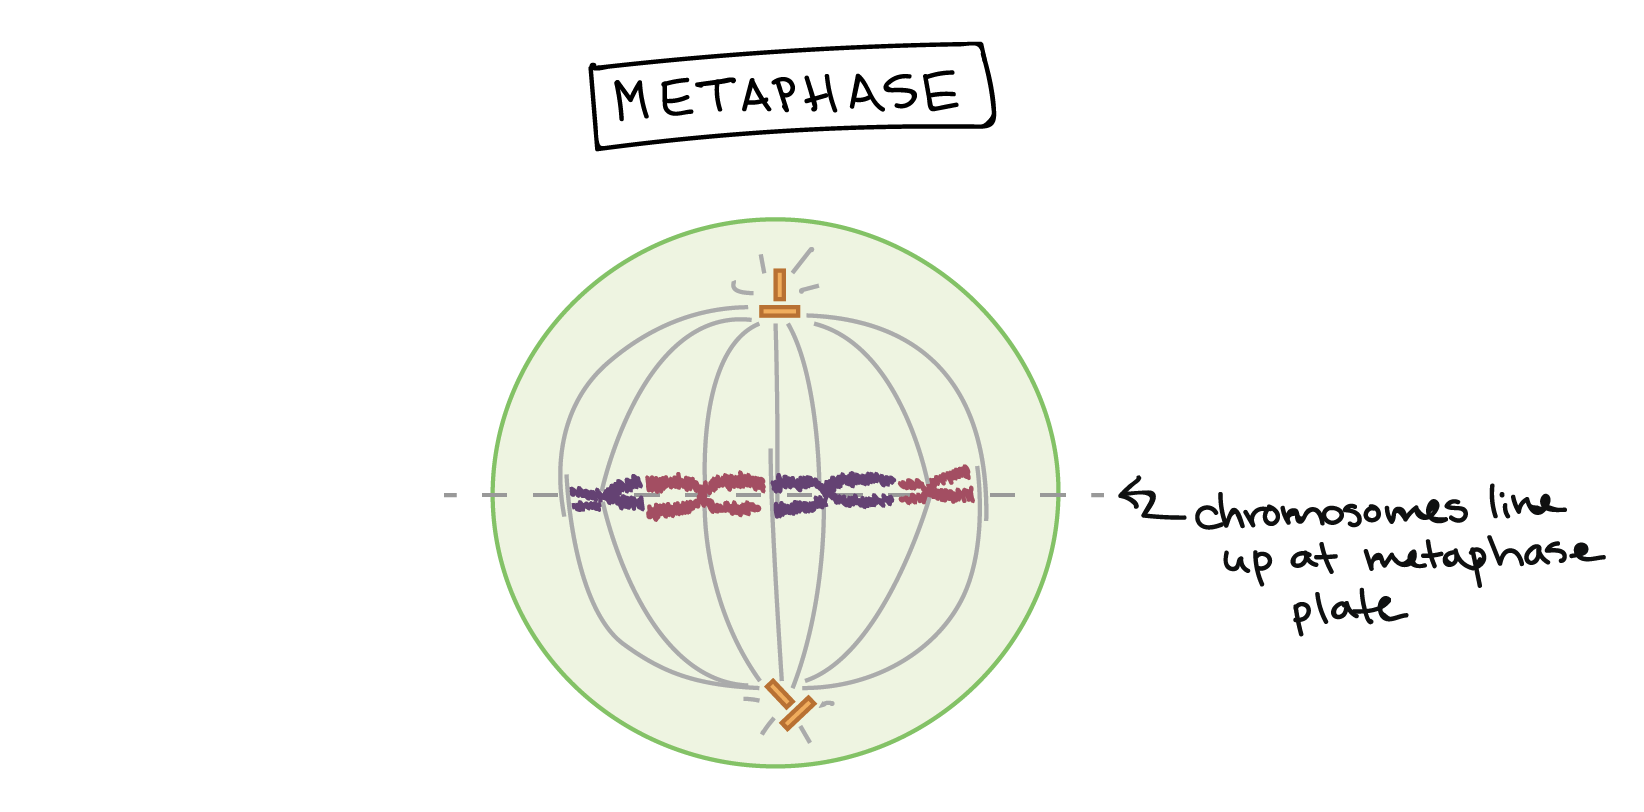
\includegraphics[width=9cm]{Metaphase}
\end{figure}

\item[\lr{Anaphase}]
طی آنافاز کروماتید‌های خواهری از هم جدا می‌شوند و با کوتاه شدن رشته‌های دوک به سمت قطب کشیده می‌شوند.

\begin{figure}[h]
	\centering
	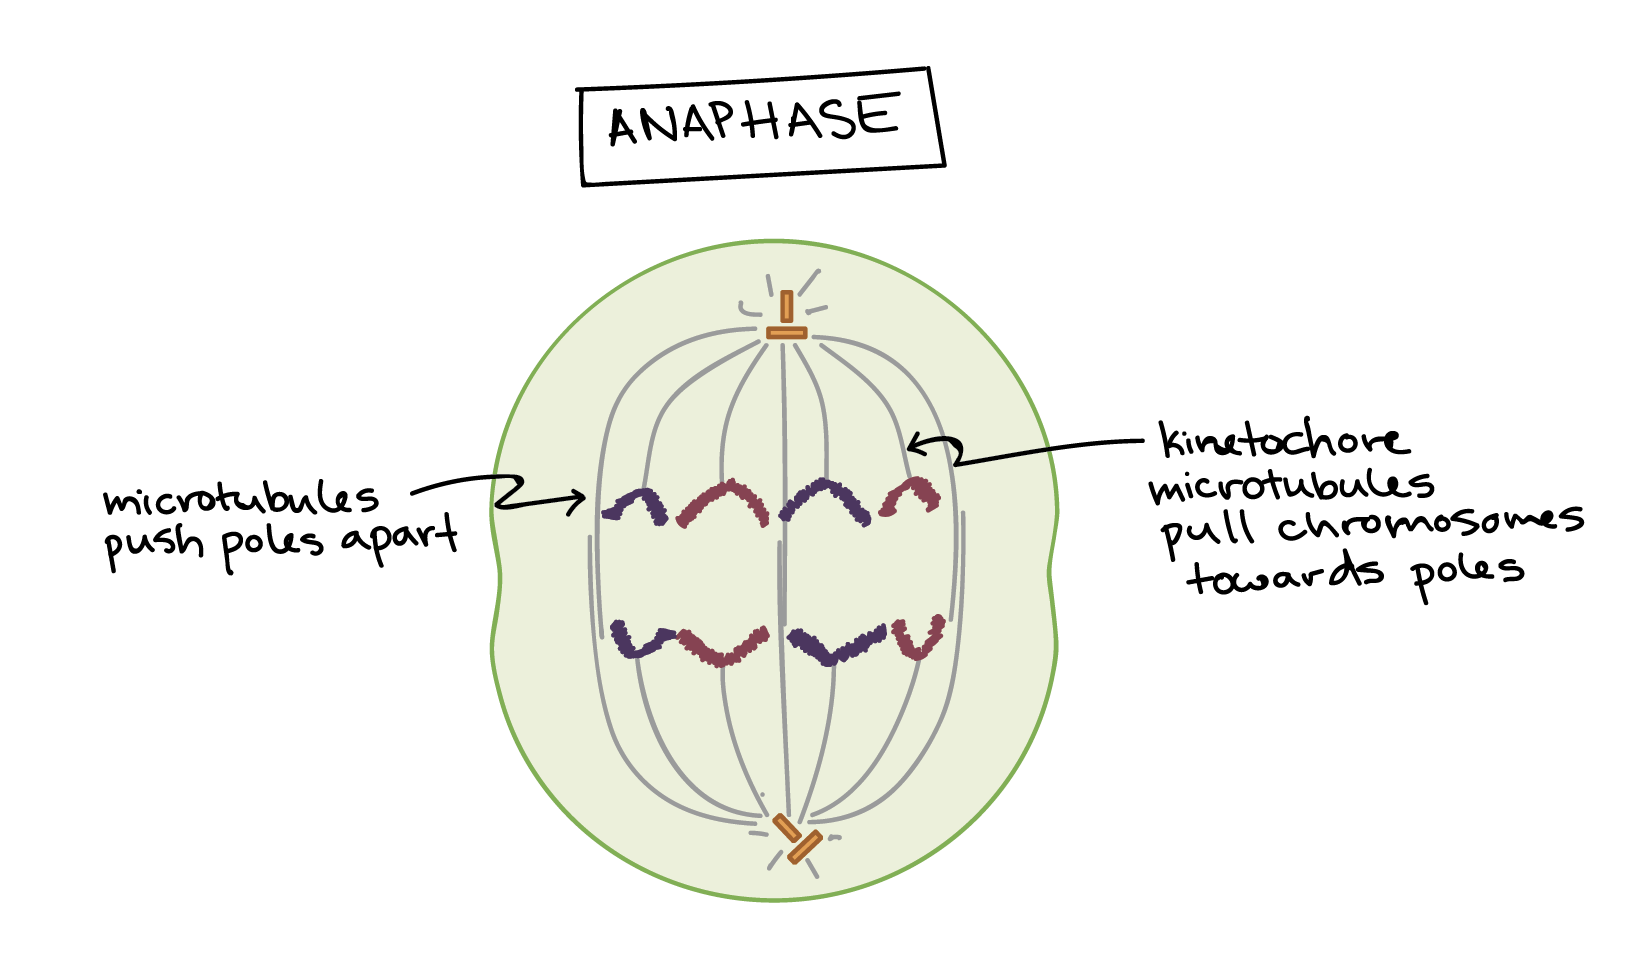
\includegraphics[width=9cm]{Anaphase}
\end{figure}

\item[\lr{Telophase}]
در هر دو قطب پوشش هسته کروموزوم‌ها را احاطه می‌کند. کروموزوم‌ها به مرور از حالت فشردگی خارج می‌شوند. رشته دوک از بین می‌رود. 

\begin{figure}[h]
	\centering
	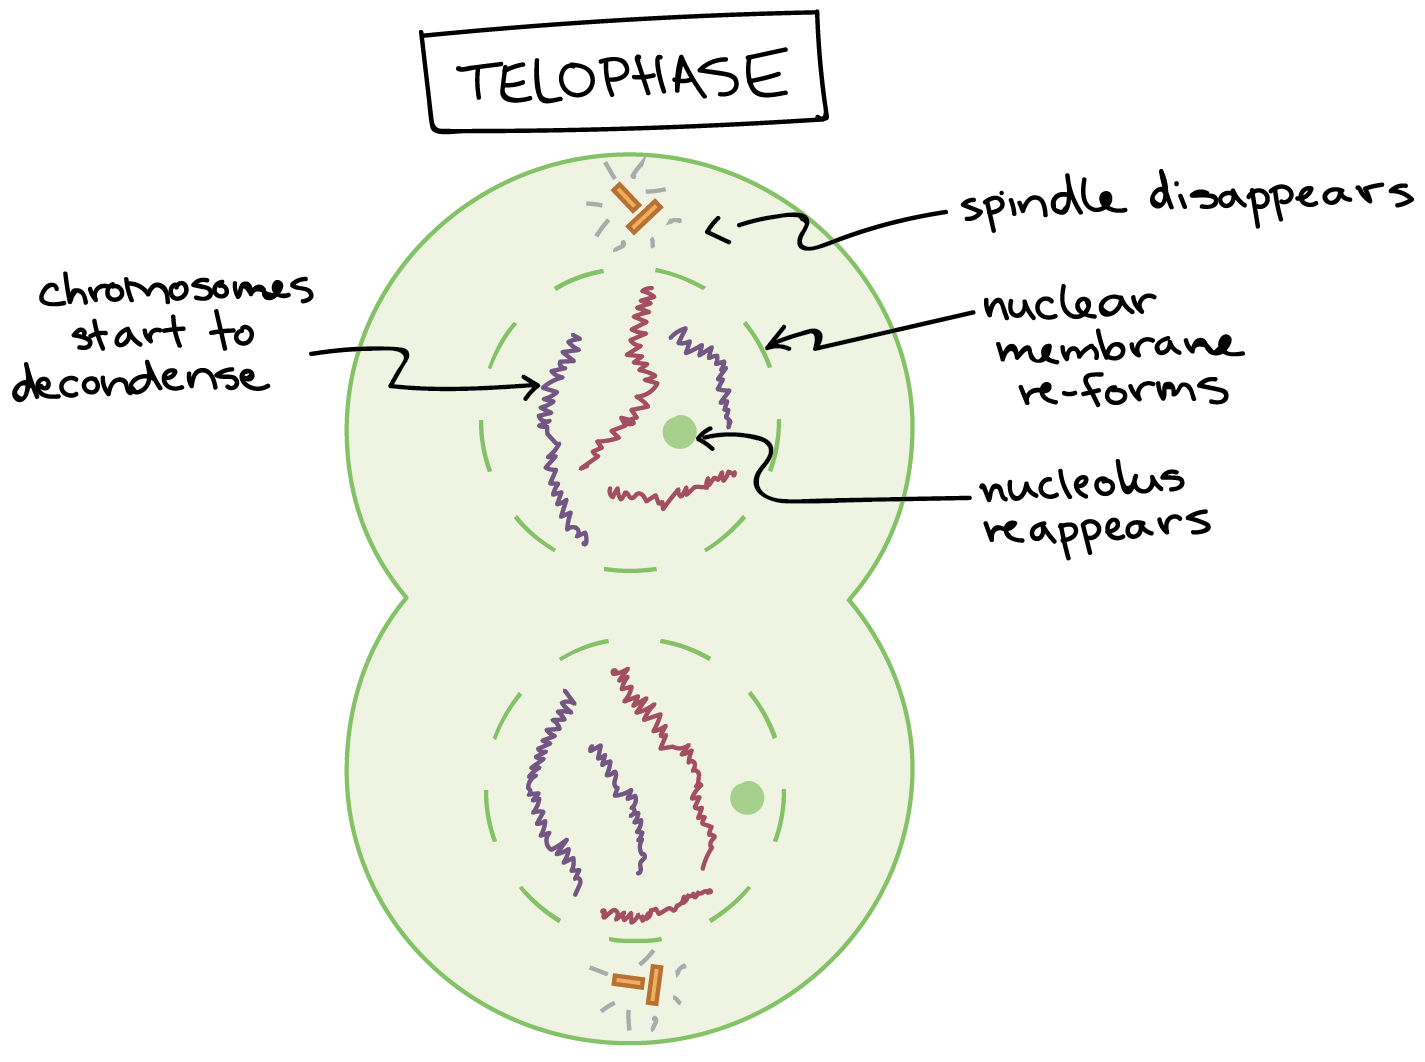
\includegraphics[width=7.5cm]{Telophase}
\end{figure}

\end{description}

\pagebreak
طی سیتوکینز غشا سلول مادری به دو قسمت تقسیم می‌شود و دو سلول دختری کامل می شوند. در سلول‌های جانوری و دیگر سلول‌هایی که دیواره ندارند، طی سیتوکینز، کمربندی از رشته‌های پروتئینی در میان سلول شکل می‌گیرد که با تنگ شدن آن سلول به دو نیمه تقسیم می‌شود. در سلول‌های گیاهی وزیکول‌هایی که توسط دستگاه گلژی ساخته شده‌اند به میانه سلول حرکت می‌کنند و در آنجا به یک دیگر می‌پیوندند و صفحه‌ای را پدید می‌آورند. این صفحه در واقع دیواره‌ای است که با غشا احاطه شده است.

\begin{figure}[h]
	\centering
	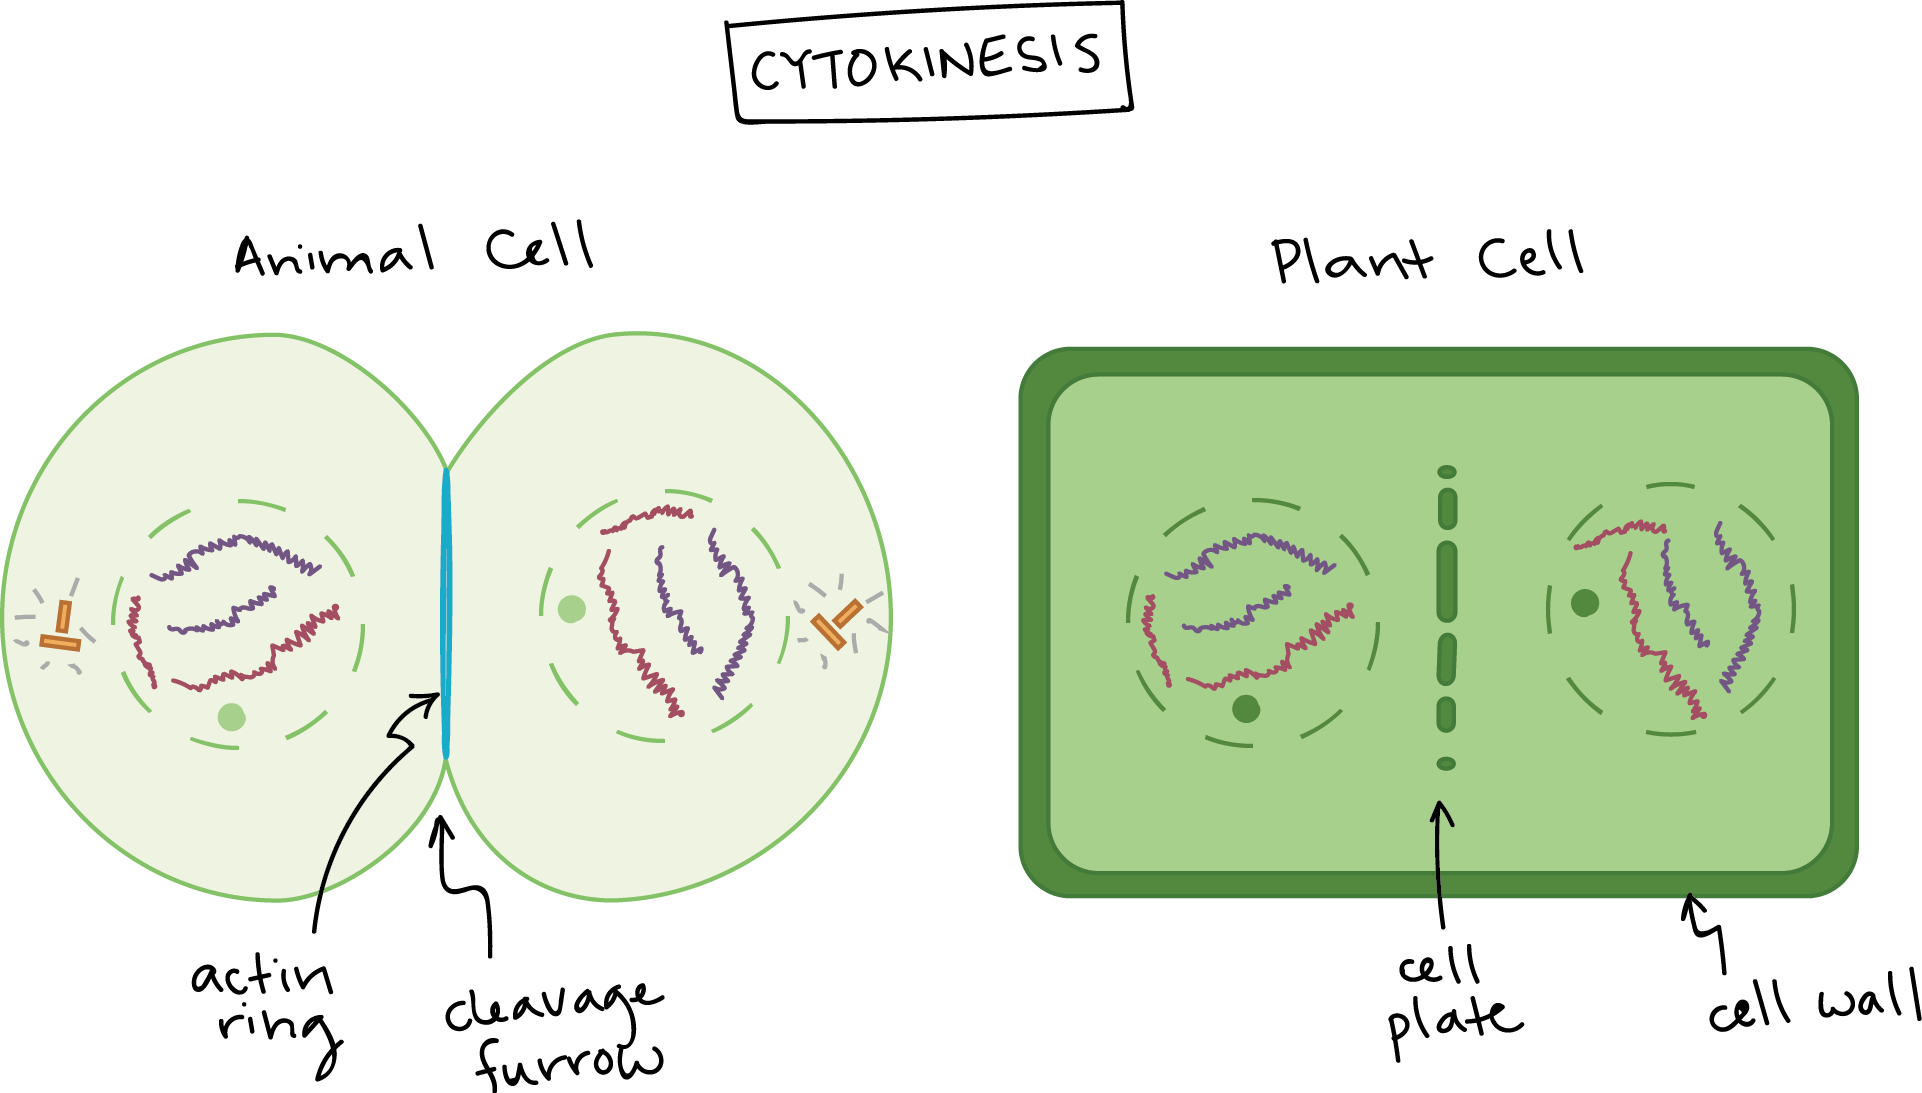
\includegraphics[width=10cm]{Cytokenesis}
\end{figure}

\pagebreak
\subsubsection{تقسیم سلولی میوز\protect\footnote{\lr{Meiosis}}}

تقسیم میتوز سلول‌های دختری ایجاد می‌کند که عینا شبیه به سلول مادر هستند. این تقسیم استفاده‌های مختلفی دارد به عنوان مثال هنگام رشد یا ترمیم زخم. اما میوز تنها با یک هدف استفاده می‌شود و آن تولید گامت
\footnote{\lr{Gamete}}
(سلول جنسی و یا اسپرم
\footnote{\lr{Sperm}}
 و تخمک
 \footnote{\lr{Egg}}
 )
است. با تقسیم میوز سلول‌های دختري به وجود می‌آید که دقیقا نیمی از کروموزوم‌های مادری را دارند.
در انسان، میوز، سلول دیپلوئیدی
\footnote{\lr{Diploid}}
را به دو سلول هاپلوئیدی
\footnote{\lr{Haploid}}
تقسیم می‌کند.

تقسیم میوز از بسیاری جهات همانند تقسیم میتوز است. با این حال تقسیم میوز پیچیده‌تر است چرا که علاوه براین که همانند تقسیم میتوز باید کروماتید‌های خواهری
\footnote{\lr{Sister chromatids}}
هر کروموزوم را جدا کند، میبایست کروموزوم‌های همتا (هومولوگ)
\footnote{\lr{homologous chromosomes}}
را نیز از هم جدا کند.

تقسیم سلولی میوز در دو مرحله انجام میگیرد:
\begin{itemize}
\item میوز
\RN{1}
:
جدا کردن کروموزوم‌های همتا
\item میوز
\RN{2}
:
جدا کردن کروماتید‌های خواهری
\end{itemize}

قبل از شروع تقسیم میوز همانند تقسیم میتوز، سلول وارد مرحله اینترفاز می‌شود. در مرحله
$ G_{1} $
سلول رشد می‌کند. در مرحله
$ S $
کروموزوم‌ها همانندسازی می‌کنند.
در مرحله
$ G_{2} $
شرایط لازم برای تقسیم فراهم می‌شود.


\begin{description}
\item[\lr{Prophase \RN{1}}]
\begin{itemize}
\item[]
\item کروموزوم‌های مضاعف شده فشرده و قابل رؤیت می‌شوند.
\item غشای هسته تجزیه می‌شود.
\item کروموزوم‌های همتا عمل 
\lr{Cross over}
را انجام می‌دهند.

\begin{figure}[htbp]
	\centering
	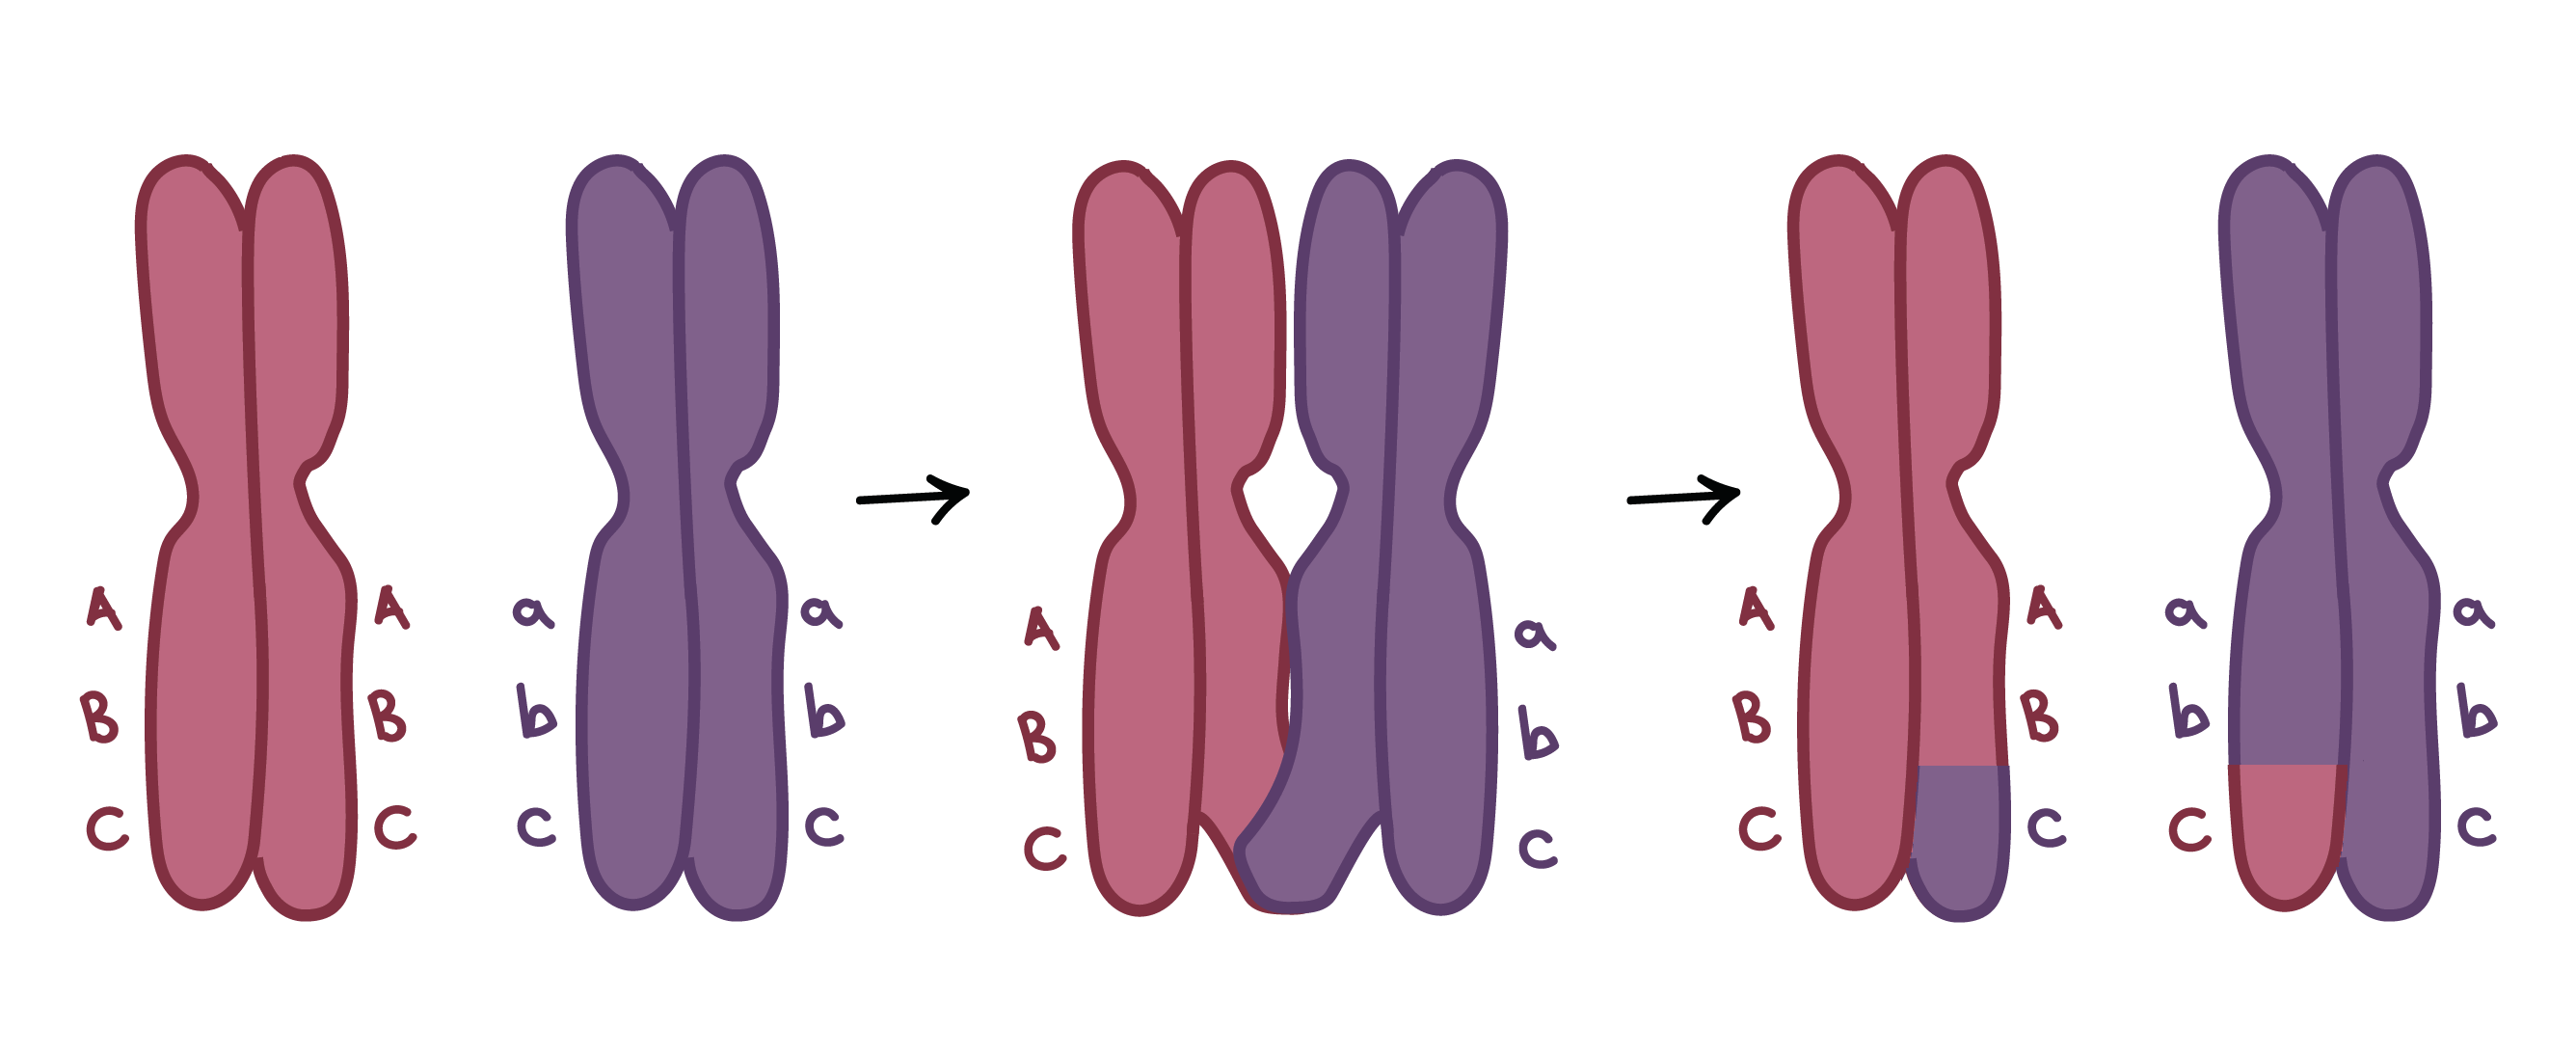
\includegraphics[width=11cm]{Cross_over}
\end{figure}

\item کروموزوم‌های همتا که هر یک دو کروماتیدی هستند از طول کنار یک دیگر قرار می‌گیرند و ساختاری را به وجود می‌آورند که تتراد 
\footnote{\lr{Tetrad}}
نام دارد. در واقع در
\lr{Cross over}
نیز کروموزوم‌ها به همین صورت هستند اما در تصویر قبل برای سادگی این طور نمایش داده شده است. شکل
\ref{figure:HomologuesChromosomes}
را مشاهده کنید. بیش‌ از یک
\lr{Cross over}
هم اتفاق می‌افتد حتی تا
$ 25! $
.
نقاطی که در آن‌ها
\lr{Cross over}
اتفاق می‌افتد کم و بیش تصادفی هستند.


\begin{figure}[htbp]
	\centering 
	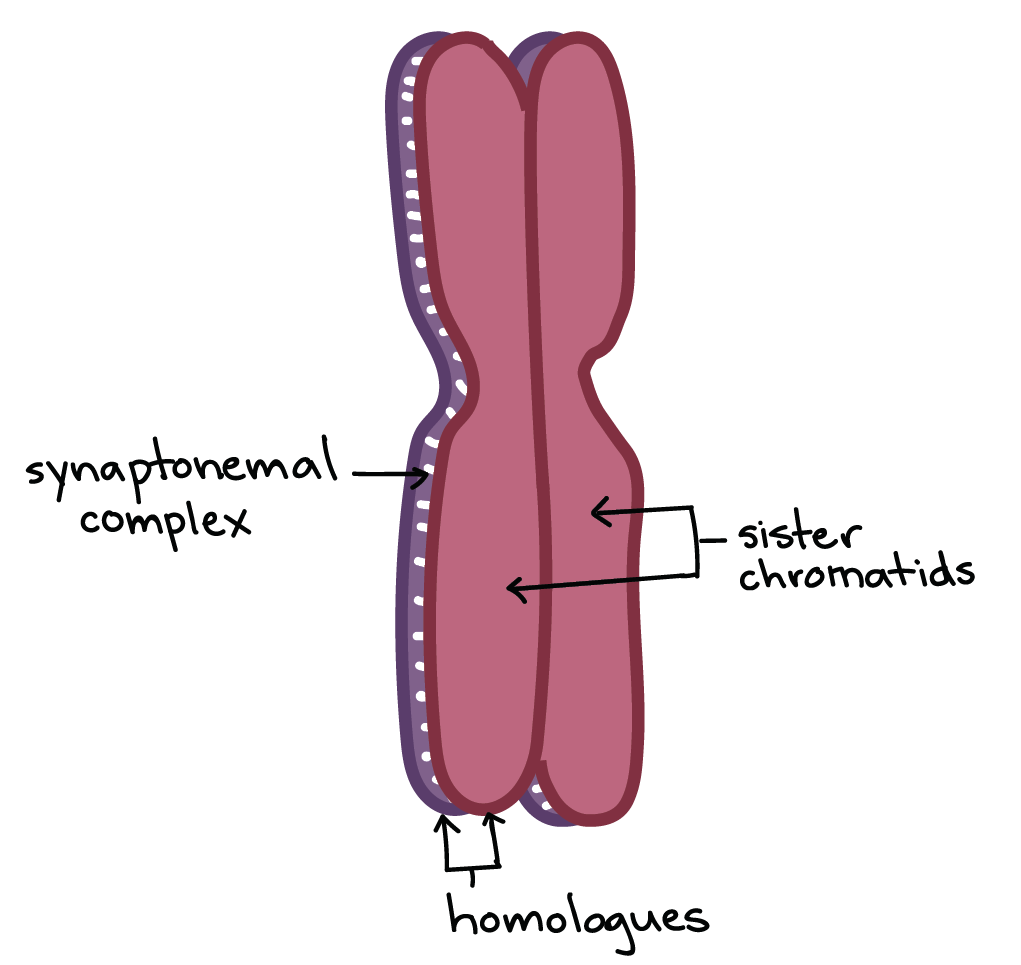
\includegraphics[width = 6cm]{Homologues_chromosomes}
	\caption{کروموزوم‌های همتا که در مرحله پروفاز
	کنار هم قرار گرفته اند}
	\label{figure:HomologuesChromosomes}
\end{figure}

\end{itemize}
\item[\lr{Metaphase \RN{1}}]
\begin{itemize}
\item[]
\item تتراد‌ها به وسیله رشته‌های دوک در سطح استوایی سلول ردیف می‌شوند.
\item ترتیب کروموزوم‌های همتا تصادفی است و به همین علت گامت‌هایی با اطلاعات ژنتیکی متفاوت ایجاد می‌شوند.
\end{itemize}
\item[\lr{Anaphase \RN{1}}]
\begin{itemize}
\item[]
\item در این مرحله کروموزوم‌های همتا از یکدیگر جدا میشوند و هر یک به سمت قطب کشیده‌ می‌شوند.
\end{itemize}

\pagebreak
\item[\lr{Telophase \RN{1}}]
\begin{itemize}
\item[]
\item رشته‌های دوک از بین می‌روند.
\item در بعضی از سلول‌ها کروموزوم‌ها را پوشش هسته احاطه می‌کند اما در بعضی دیگر این کار انجام نمی‌شود چرا که سلول وارد تقسیم بعدی می‌شود.
\item در هر یک از هسته‌ها عدد جنسی نصف شده است چرا که از هر کروموزوم همتا فقط یکی وجود دارد.
\end{itemize}
\end{description}

\noindent
میوز
\RN{2}
همانند تقسیم میتوز است:
\begin{description}
\item[\lr{Prophase \RN{2}}]
\begin{itemize}
\item[]
\item غشای هسته تجزیه می‌شود.
\item رشته‌های دوک تشکیل می‌شوند.
\end{itemize}
\item[\lr{Metaphase \RN{2}}]
\begin{itemize}
\item[]
\item کروموزوم‌ها به وسیله رشته‌های دوک در سطح استوایی سلول ردیف می‌شوند.
\end{itemize}
\item[\lr{Anaphase \RN{2}}]
\begin{itemize}
\item[]
\item در این مرحله کروماتید‌های یک کروموزوم از یکدیگر جدا میشوند و هر یک به سمت قطب کشیده‌ می‌شوند.
\item در این مرحله برخلاف میتوز از هر کروموزوم‌ همتا فقط یکی وجود دارد.
\end{itemize}
\item[\lr{Telophase \RN{2}}]
\begin{itemize}
\item[]
\item رشته‌های دوک از بین می‌روند.
\item کروموزوم‌ها را پوشش هسته احاطه می‌کند.
\end{itemize}
\end{description}

\begin{figure}[htbp]
	\centering
	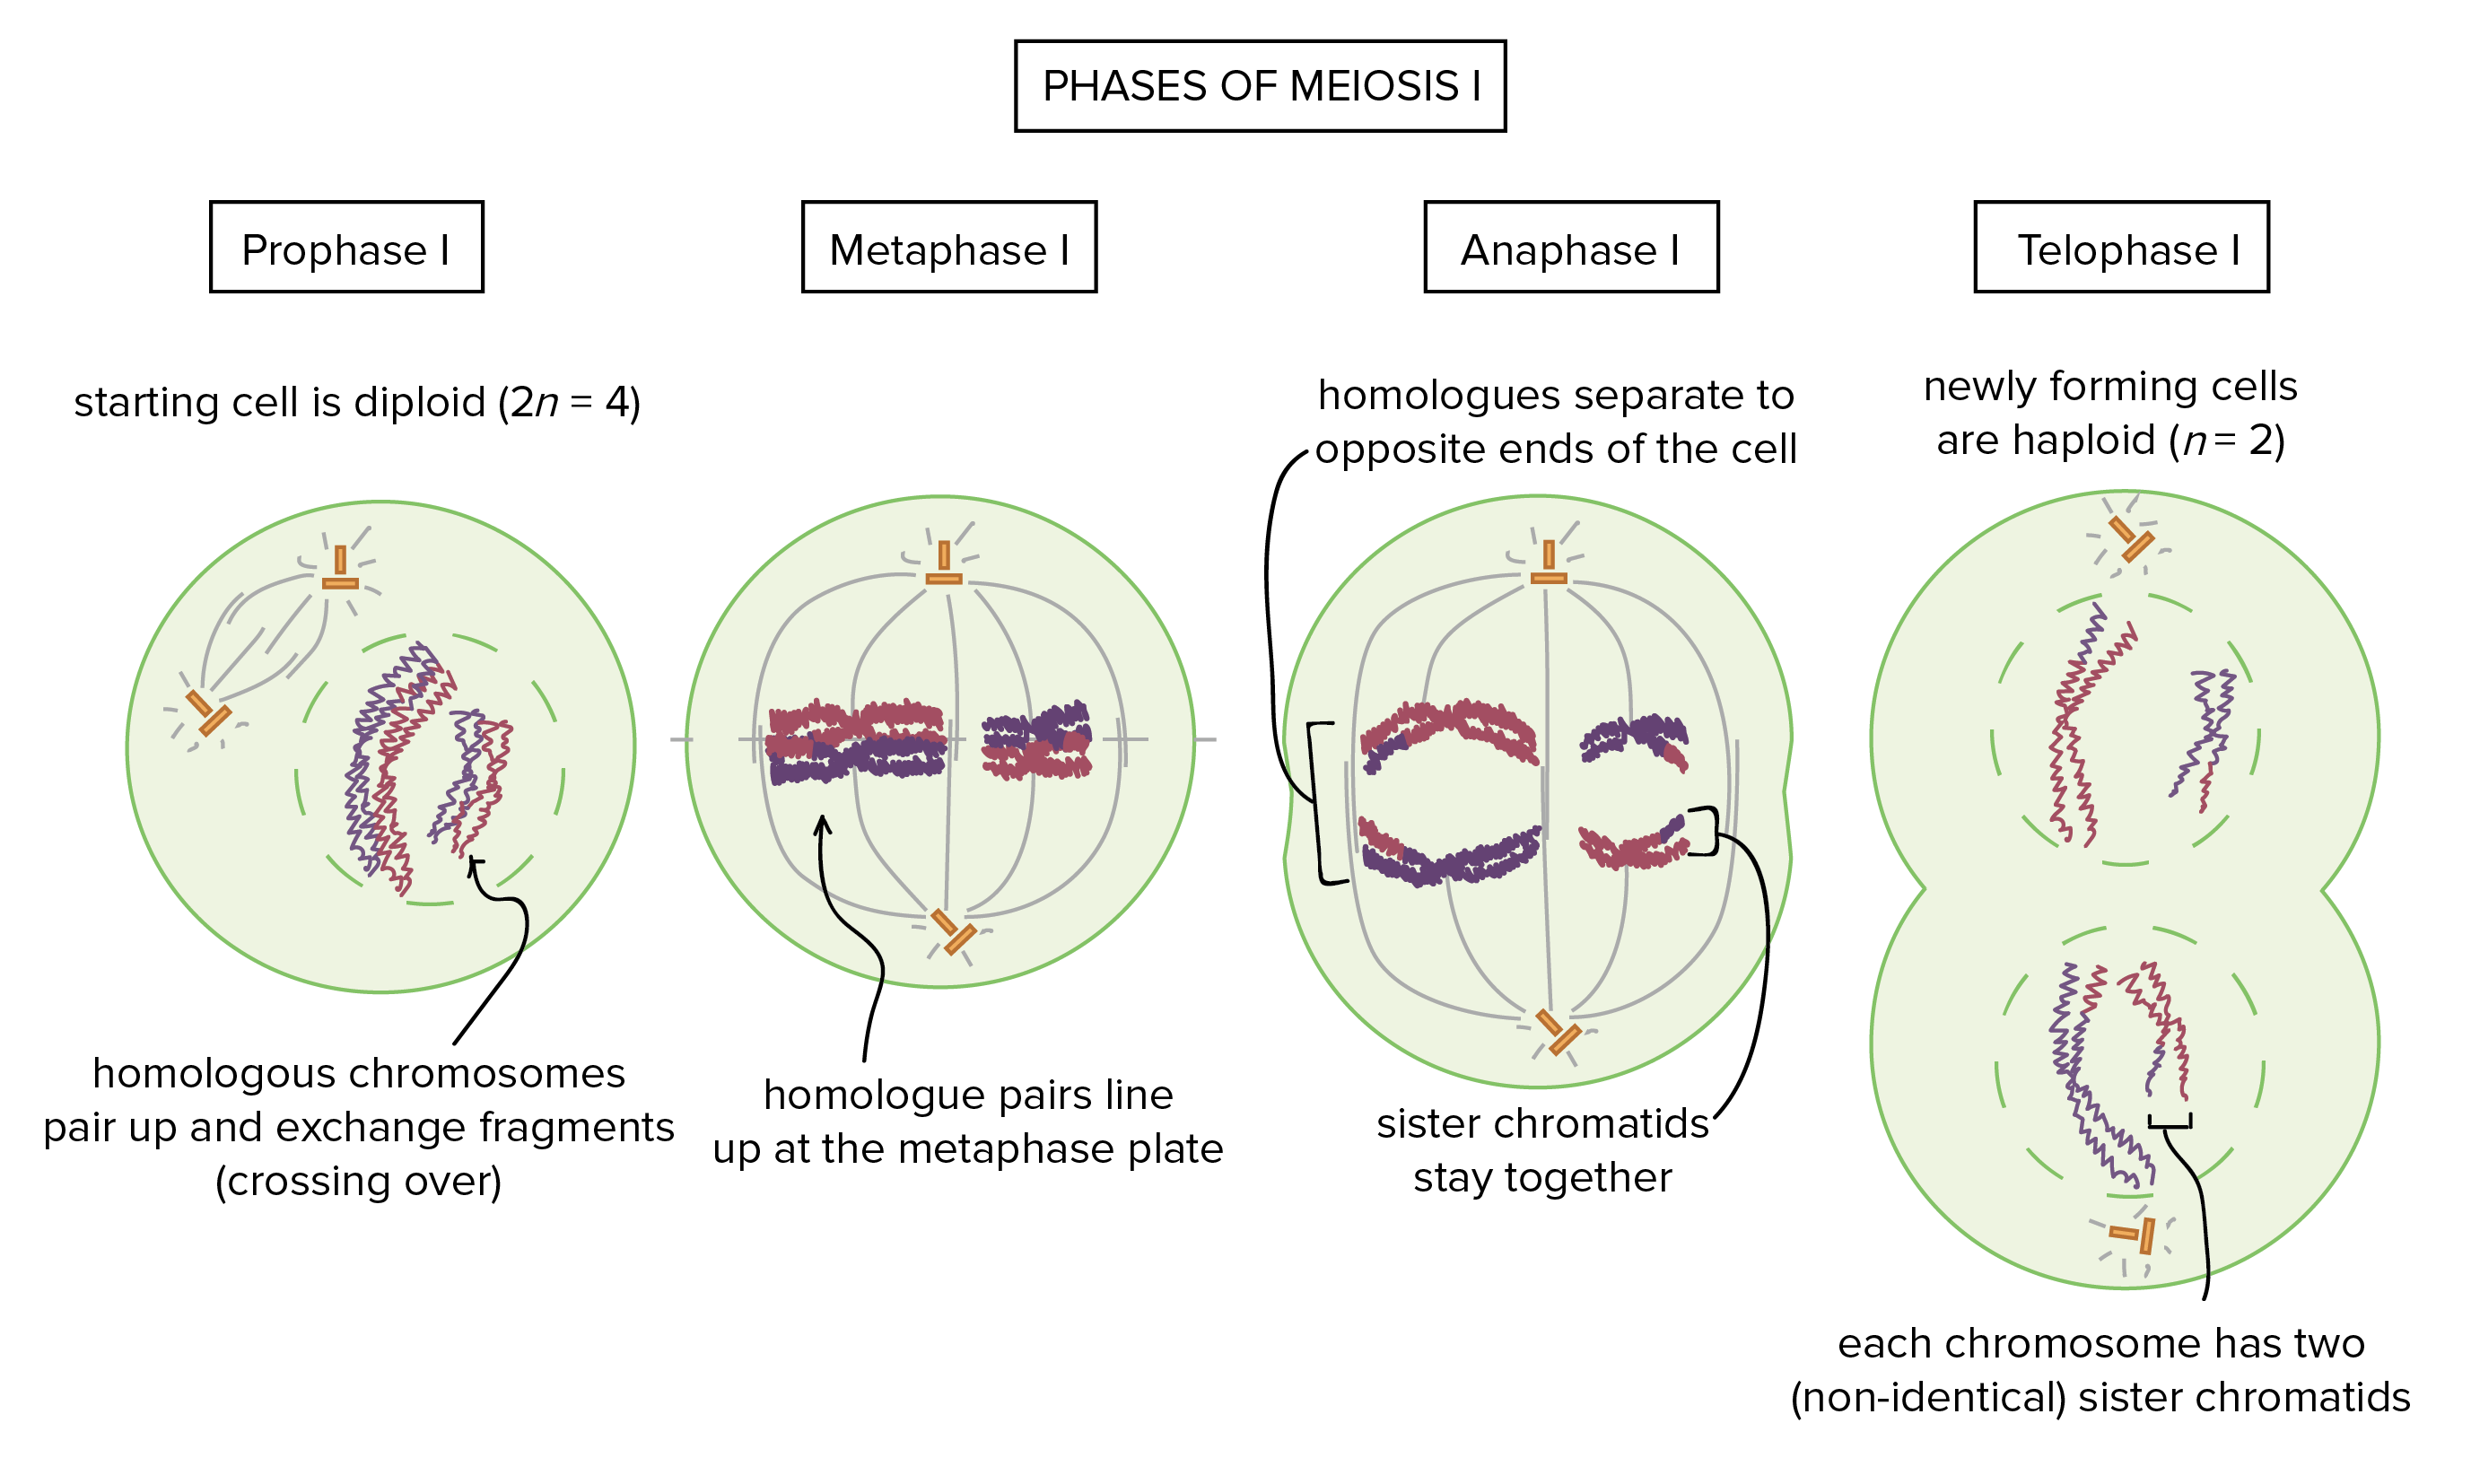
\includegraphics[width=12cm]{Meiosis_one}
	\includegraphics[width=12cm]{Meiosis_two}
	\caption{میوز
	\RN{1}
	و
	میوز
	\RN{2}}
\end{figure}

\pagebreak
\subsubsection{میوز در انسان}

همان طور که در شکل
\ref{figure:spermatogenesis}
مشاهده می‌کنید تقسیم میوز در جنس نر اسپرم‌های با اندازه مساوی ایجاد می‌کند اما در نوع ماده اینگونه نیست در واقع در هر دو مرحله از میوز تقریبا تمام سیتوپلاسم به یکی از دو سلول دختر منتقل می‌شود در نتیجه در انتها تنها یک سلول تخمک ایجاد می‌شود. سایر سلول‌های دختر به دلیل نداشتن سیتوپلاسم از بین می‌روند.

نکته دیگر درمورد انسان این است که در جنس نر اسپرم‌ها در تمام طول زندگی به وجود می‌آیند اما تخمک‌ها از بدو تولد در تخمدان هستند و بعد از این دیگر تخمکی ایجاد نمی‌شود. این نکته تخمک‌ها از ابتدا در رحم هستند باعث می‌شود که با بالاتر رفتن سن در جنس ماده احتمال آسیب دیدن آنها نیز بیشتر شود.

\begin{figure}[htbp]
	\centering
	\includegraphics[width=9cm]{spermatogenesis_oogenesis}
	\caption{تولید اسپرم و تخمک}
	\label{figure:spermatogenesis}
\end{figure}

\subsubsection{کروموزوم‌های جنسی}
در انسان 23 جفت کروموزوم وجود دارد. از این 23 جفت کروموزوم 22 جفت غیر جنسی است که به آنها
\lr{autosome}
می‌گویند
و هر جفت از این 22 جفت نسبت به هم
\lr{Homologous}
هستند اما کروموزوم‌های جنسی
\footnote{\lr{sex chromosomes}}
 ممکن است
\lr{Homologous}
باشند یا نباشند. به عنوان مثال در انسان جنس نر دارای کروموزوم‌های جنسی $ X $
و
$ Y $
است که نسبت به هم همولوگ نیستند اما در جنس ماده کروموزوم‌های جنسی
هر دو
$ X $
هستند که همولوگ می‌باشند.
به جنس ماده
\lr{Homogametic}
می‌گویند چرا که تنها یک نوع گامت از نظر کروموزوم جنسی تولید می‌کند و به جنس نر
\lr{Heterogametic}
می‌گویند چرا که از نظر جنسی دو نوع گامت تولید می‌کند.

\pagebreak
\subsubsection{مولکول آر ان ای}
همانطور که قبلا گفته شد
\lr{RNA}
یک نوع
\lr{nucleic acid}
و یا همان اسید هسته‌ای است که به علت داشتن قند ریبوز به آن
\lr{ribonucleic acid}
گفته می‌شود. در گذشته تصور می‌شد تنها کاری که مولکول
\lr{RNA}
انجام می‌دهد، رونویسی از مولکول
\lr{DNA}
است اما امروزه میدانیم که
\lr{RNA}
ها ساختار سه‌بعدی مهمی دارند و کارهای عملکردی انجام می‌دهند. در واقع
\lr{RNA}
چیزی بین
\lr{DNA}
و پروتئین است. یک تئوری برای آغاز حیات در دنیا این است که حیات با مولکول
\lr{RNA}
آغاز شده است و بعد از آن این مولکول تصمیم گرفته است که
\lr{DNA}
را به وجود آورد. به این تئوری
\lr{RNA World}
گفته می‌شود.

نکته‌ای که درمورد
\lr{RNA}
وجود دارد این است که بر خلاف مولکول
\lr{DNA}
اغلب به صورت تک
\lr{Strand}
است. 
\lr{RNA}
در هسته سنتز می‌شود. بعد از سنتز
\footnote{\lr{synthesis}}
بیشتر
\lr{RNA}
ها به سیتوپلاسم مهاجرت می‌کنند. زیست‌شناسان برای آن که میزان بیان یک ژن را بسنجند میزان
\lr{RNA}
هایی که از روی آن ژن رونویسی شده است را اندازه می‌گیرند چرا که نمی‌توانند این کار را از روی پروتئین‌های مربوط به یک ژن انجام دهند. پروتئین‌ها اندکی بعد از ساخته شدن و انجام وظیفه خود، نابود می‌شوند به همین علت نمی‌توان مقدار آن‌ها را به طور دقیق اندازه گیری کرد.

\begin{table}[htbp]
	\centering
	\begin{tabular}{|c|c|}
	\hline
	\lr{DNA} & \lr{RNA} \\ \hline
	نوکلئوتید‌ها دارای قند دئوکسی ریبوز می‌باشند.
	&
	نوکلئوتید‌ها دارای قند ریبوز می‌باشند.
	\\
	\hline
	دارای نوکلئوتید تیمین می‌باشد.
	&
	دارای نوکلئوتید یوراسیل می‌باشد.
	\\
	\hline
	به صورت
	\lr{double strand}
	است.
	&
	اغلب به صورت
	\lr{single strand}
	است.
	\\
	\hline
	تنها، منبع ذخیره ژن است.
	&
	معمولا ساختار پیچیده سه‌بعدی به خود می‌گیرد و عملکرد‌های متفاوتی دارند.
	\\	
	\hline
	
	\end{tabular}
\end{table}

\subsubsection{رونویسی\protect\footnote{\lr{Transcription}}}
